%\documentclass[11pt,a4paper]{article}
%\documentclass[11pt,a4paper]{scrartcl}
\documentclass[11pt,a4paper,oneside]{book}
\usepackage[british,UKenglish,USenglish,english,american]{babel}
%\usepackage[a4paper, total={16cm, 23cm}]{geometry}
\usepackage[tmargin = 1.25in,bmargin = 1.25in,lmargin = 1in,rmargin = 
1in]{geometry}
\usepackage{tikz}
\usepackage{graphicx}
\usepackage{pgfplots}
\pgfplotsset{width=12cm,compat=1.9}

\usepackage{chemmacros}
\usepackage{chemfig}
%\usepackage{ghsystem}
%\usechemmodule{redox}
%\usepackage{chemnum}
%\usepackage{bohr}
%\usepackage{elements}
%\usepackage{endiagram}
%\usepackage{modiagram}
%\usepackage{chemgreek}
%\usepackage{mhchem}
\usepackage{esint}
\usepackage{tabularray}

\usepackage{makeidx}
\usepackage{epstopdf}

\usepackage{amssymb}
\usepackage{mathrsfs}
%\usepackage{minted}
\usepackage{bm}
\usepackage{amsmath}
\usepackage{enumitem}
\usepackage[english]{varioref}
\usepackage[english]{babel}
\usepackage{lipsum}
\usepackage{fancyhdr}
\pagestyle{fancy} 
\usepackage{float}
\usepackage{empheq}
\usepackage[framemethod=tikz]{mdframed}
\usepackage{epstopdf}
\numberwithin{equation}{section}
\usepackage{eso-pic}
\usepackage{calc}
\usepackage{nccmath}
\usepackage{caption}
\usepackage{subcaption}
\usepackage{gensymb}
\usepackage{amsfonts,amsthm,epsfig,epstopdf,titling,url,array}
\usepackage{siunitx}
\sisetup{input-digits = 0123456789\pi}
\usepackage[symbol]{footmisc}
\usepackage{xcolor}
\usepackage{multicol}
\usepackage{boondox-cal}
\DeclareSIUnit\atm{atm}
\setcounter{secnumdepth}{3}
\setcounter{tocdepth}{3}
\usepackage{booktabs}
\usepackage{blindtext}
\usepackage{changepage}

% \usepackage{draftwatermark}
% \SetWatermarkText{DRAFT}
% \SetWatermarkScale{5}

\DeclareSIUnit\atm{atm}

\pagestyle{fancy} 
\fancypagestyle{firstpage}{
	\rhead{
		%	\begin{picture}(0,0) 
			%			\put(-30,0){
\includegraphics[width=1cm]{figures/MCI_4C_bw.eps}} 
			%	\end{picture}
	}
}
\fancyhead[L]{\slshape\nouppercase{\leftmark}}
\chead{}
\rhead{
	%	\begin{picture}(0,0) 
		%		\put(-30,0){
\includegraphics[width=1cm]{figures/MCI_4C_bw.eps}} 
		%	\end{picture}
}
\lfoot{\textit{}}
\cfoot{-\ \thepage\ -}
\rfoot{\textit{}}

\DeclareMathOperator{\rank}{rank}
\DeclareMathOperator{\atantwo}{atan2}
\DeclareMathOperator{\spn}{span}

\renewcommand{\headrulewidth}{0.4pt}
\renewcommand{\footrulewidth}{0.4pt}
\newcommand{\abs}[1]{\left|#1\right|}
\definecolor{mycolor1}{rgb}{0.97, 0.97, 0.97}
\definecolor{mycolor2}{rgb}{0.97, 0.97, 0.97}
\definecolor{tableShade}{gray}{0.9}
\newcommand{\sign}{\text{sign}}
\newcommand{\centered}[1]{\begin{tabular}{@{}l@{}} #1 \end{tabular}}
\theoremstyle{it}
\newtheorem{defn}{Definition}[chapter]
\newtheorem{assumption}{Assumption}[chapter]
\newtheorem{thm}{Theorem}[chapter]
\newtheorem{lemma}{Lemma}[chapter]
\newtheorem{corollary}{Corollary}[chapter]
\theoremstyle{definition}
%\theoremstyle{it}
\newtheorem{example}{Example}[section]

\newenvironment{myitemize_1}
{ \begin{itemize}[topsep=0pt]
		\setlength{\topsep}{2pt}		
		\setlength{\itemsep}{2pt}
		\setlength{\parskip}{2pt}
		\setlength{\parsep}{2pt}     }
	{ \end{itemize}                  }


\newmdenv[innerlinewidth=0.5pt, roundcorner=4pt,backgroundcolor=mycolor2, 
linecolor=mycolor1,innerleftmargin=6pt,
innerrightmargin=6pt,innertopmargin=6pt,innerbottommargin=6pt]{mybox}


\title{\textbf{Theory of Electromechanical Devices}}
\author{\textbf{Davide Bagnara}}

\begin{document}
	\thispagestyle{firstpage}
	\begin{mybox}
		\maketitle
		\vspace{145mm}
	\end{mybox}
	\newpage
	\tableofcontents
	\listoffigures	
	\listoftables

\chapter{Review of Maxwell's equations}
\section{Maxwell's equations}
Electromagnetic fields arise from source of charge and current and are governed by Maxewell's equations. The field equations in differential form are as follows,
 \begin{equation}\label{maxwell_1}
 	\vec{\nabla}\times\vec{H}=\vec{J} + \frac{\partial \vec{D}}{\partial t}
 \end{equation}
\begin{equation}\label{maxwell_2}
	\vec{\nabla}\cdot\vec{B}=0
\end{equation}
 \begin{equation}\label{maxwell_3}
	\vec{\nabla}\times\vec{E}=- \frac{\partial \vec{B}}{\partial t}
\end{equation}
\begin{equation}\label{maxwell_4}
	\vec{\nabla}\cdot\vec{D}=\rho
\end{equation}
In these equations $\vec{J}$ $\big(\SI{}{\ampere\per\square\meter}\big)$ and $\rho$ $\big(\SI{}{\coulomb\per\cubic\meter}\big)$ are source terms and $\vec{H}$, $\vec{B}$, $\vec{E}$ and $\vec{D}$ are the fields. These are defined as follows:
\begin{center}
\boxed{	\begin{tabular}{ c c }
\text{Field} & \text{Description} \\[8pt] 
$\vec{E}$ & \text{Electric field intensity $\big(\SI{}{\volt\per\meter}\big)$} \\[8pt]  			$\vec{D}$ & \text{Electric flux density $\big(\SI{}{\coulomb\per\square\meter}\big)$} \\[8pt]  			
$\vec{H}$ & \text{Magnetic field intensity $\big(\SI{}{\ampere\per\meter}\big)$} \\[8pt]  
$\vec{B}$ & \text{Magnetic flux density $\big(\SI{}{\weber\per\square\meter}\big)$}    
\end{tabular}}
\end{center}
The fields are vector-valued functions of space and time, e.g. the field $\vec{B}$ can be represented as follows $$ \vec{B} = B_x\big(x,y,z,t\big)\vec{i}+B_y\big(x,y,z,t\big)\vec{j}+B_z\big(x,y,z,t\big)\vec{k}$$ as each of the four fields has three components, the field equations represent a system equations for 12 unknown field components. However, while these equations are consistent, they are not all independent. Therefore they do not provide the 12 independent scalar equations required to determine the 12 unknown. Specifically the two divergence equations can be obtained from the two curl equations if one imposes the continuity of charge equation. Thus, for a complete theory the field equations must be augmented by additional independent equations that take the form of \textbf{constitutive relations}. The source terms in the field equations are the free current density and the free charge density. The field equations embody the conservation of free charge as expressed by the continuity equation
\begin{equation}\label{continuity}
	\vec{\nabla}\cdot\vec{J}+\frac{\partial \rho}{\partial t}=0
\end{equation}
This is obtained by combining the divergence of Eq.~\eqref{maxwell_1} with the time derivative of Eq.~\eqref{maxwell_4}. On the other hand, if Eq.~\eqref{continuity} is viewed as an independent equation, we find that the two divergence equations \ref{maxwell_2} and \ref{maxwell_4} can be obtained from the two curl equations \ref{maxwell_1} and \ref{maxwell_3}.

In addition to free charge there is also bound charge. Bound charge is charge that is displaced from its atomic or molecular source, but does not separate from it. Bound charge arise during the polarization of dielectric materials. The term $\partial\vec{D}/\partial t$ in Eq.~\eqref{maxwell_1} is called the displacement current density and accounts for the motion of bound charge.
\subsection{Constitutive relations}
As already noted, Maxwell's equations by themselves do not provide a complete set of equations for the fields. To complete the theory, the field equations must be augmented by additional independent equations that are specific by the following constitutive relations:
\begin{equation}\label{constitutive_1}
	\vec{B}=\mu_0\Big(\vec{H}+\vec{M}\Big)
\end{equation}
\begin{equation}\label{constitutive_2}
	\vec{D}=\epsilon_0\vec{E}+\vec{P}
\end{equation}
where $\vec{M}$ $\big(\SI{}{\ampere\per\meter}\big)$ is the magnetization, $\vec{P}$ $\big(\SI{}{\coulomb\per\square\meter}\big)$ is the polarization and $$\mu_0 = \SI{4\pi e-7}{\weber\per\meter\per\ampere}$$ and $\epsilon_0= \SI{8.854e-12}{\farad\per\meter}$ are the permeability and permittivity of free space, respectively.

The magnetization $\vec{M}$ represents the net magnetic dipole moment per unit volume of a material. Specifically, $\vec{M}$ is given by
 \begin{equation}\label{}
 	\vec{M}=\lim_{\Delta V\rightarrow 0}\frac{\sum_{i}\vec{m}_i}{\Delta V}
 \end{equation}
where $\sum_{i}\vec{m}_i$ is a vector sum of the magnetic dipole moments contained in the elemental volume $\Delta V$. 

Similarly, polarization $\vec{P}$ represents the net electric dipole moment per unit volume. It is given by
  \begin{equation}\label{}
 	\vec{P}=\lim_{\Delta V\rightarrow 0}\frac{\sum_{i}\vec{p}_i}{\Delta V}
 \end{equation}
where $\sum_{i}\vec{p}_i$ is a vector sum of the electric dipole moments contained in the elemental volume $\Delta V$.

In stationary, linear, homogeneous and isotropic media the constitutive relations reduce to
\begin{equation}\label{constitutive_3}
	\vec{B}=\mu\vec{H}
\end{equation}
\begin{equation}\label{constitutive_4}
	\vec{D}=\epsilon\vec{E}
\end{equation}
where $\mu$ and $\epsilon$ are the permeability and permittivity of the media respectively. There is an additional constitutive relation that relates $\vec{J}$ to $\vec{E}$
\begin{equation}\label{constitutive_5}
	\vec{J}=\sigma\vec{E}
\end{equation}
where $\sigma$ is the conductivity with units $\SI{}{\ampere\per\volt\meter}$.
The constitutive relations needs to be defined also for nonlinear, inhomogeneou or anisotropic materials. A material is nonlinear if $\mu$, $\epsilon$ or $\sigma$ depend on the fields, otherwise it is linear. For nonlinear materials the constitutive equations can be written as follows
\begin{equation}\label{constitutive_6}
	\vec{B}=\vec{\vec{\mu}}(H)\vec{H}
\end{equation}
\begin{equation}\label{constitutive_7}
	\vec{D}=\vec{\vec{\epsilon}}(E)\vec{E}
\end{equation}
\begin{equation}\label{constitutive_8}
	\vec{J}=\vec{\vec{\sigma}}(E)\vec{E}
\end{equation}
\subsection{Integral equations}
The integral form of the field equations is obtained as follows: take the surface integral of the curl equations \ref{maxwell_1} and \ref{maxwell_3} over an open surface $S$ bounded by a contour $C$ and then apply Stokes theorem to the left-hand side and obtain
 \begin{equation}\label{maxwell_int_1}
	\oint_C\vec{H}\cdot d\vec{l}=\int_S\Big(\vec{J} + \frac{\partial \vec{D}}{\partial t}\Big)\cdot d\vec{a}
\end{equation}
\begin{equation}\label{maxwell_int_2}
	\oint_{C}\vec{E}\cdot d\vec{l}=-\int_{S}\frac{\partial \vec{B}}{\partial t}\cdot d\vec{a}
\end{equation}
Similarly, integrate the divergence equations \ref{maxwell_2} and \ref{maxwell_4} over a volume $V$ with a closed surface $S$ and then apply the divergence theorem to the left-hand side. This gives
\begin{equation}\label{maxwell_int_3}
	\oint_{S}\vec{B}\cdot d\vec{a}=0
\end{equation}
\begin{equation}\label{maxwell_int_4}
	\oint_{S}\vec{D}\cdot d\vec{a}=\int_{V}\rho dv
\end{equation}
respectively. Equations \eqref{maxwell_int_1}~-~\eqref{maxwell_int_4} constitute the integral form of the field equations. The first equation \eqref{maxwell_int_1} is a generalization of Ampere's circuital law, which states that the circulation of the magnetic field intensity around any closed path is equal to the free current flowing through the surface bounded by the path.

The second equation Eq.~\eqref{maxwell_int_2} is a generalization of the Faraday's law of electromagnetic induction, which states that the electromotive force induced in a stationary closed circuit equals the negative rate of increase of the magnetic flux linking the circuit. In simpler terms, this law states that an $\vec{E}$-field is generated by a time-varying magnetic flux. The negative sign in Eq.~\eqref{maxwell_3} implies that the induced $\vec{E}$-field will act to oppose the change in magnetic flux. This is known as Lenz's law. Faraday's law provides the basis for the behavior of many important devices including transformers, generators and electromechanical devices.

The third equation \ref{maxwell_int_3} states that the total outward flux of the $\vec{B}$-field over a closed surface equals to zero. Recall that the flux of a vector field $\vec{B}$ through a surface $S$ is defined by, 
\begin{equation*}\label{}
	\phi = \underbrace{\int_{S}\vec{B}\cdot d\vec{a}}_{\text{Flux of $\vec{B}$ through $S$}}
\end{equation*}
Eq.~\eqref{maxwell_int_3} implies that there are no isolated source or sinks of magnetic field, that is, no magnetic monopoles. 

The fourth equation \eqref{maxwell_int_4} is Gauss's law. It states that the total outward flux of the $\vec{D}$-field over a closed surface equals the total free charge enclosed by the surface. 

The differential and integral form of Maxwell's equations are summarized in Table~\ref{summary}.
\begin{table}
\centering \textbf{Maxwell's Equations} \\
	\begin{align*}
		\hline \\
		&\text{Differential Form} 	& 	&\text{Integral form} \\[24pt] 
		&\vec{\nabla}\times\vec{H}=\vec{J} + \frac{\partial \vec{D}}{\partial t}	& 	
		&\oint_C\vec{H}\cdot d\vec{l}=\int_S\Big(\vec{J} + \frac{\partial \vec{D}}{\partial t}\Big)\cdot 	d\vec{a}		\\[24pt]  
		&\vec{\nabla} \cdot\vec{B}=0	&
		&\oint_{S}\vec{B}\cdot d\vec{a}=0 \\[24pt] 
		&\vec{\nabla}\times\vec{E}=- \frac{\partial \vec{B}}{\partial t}	&	
		&\oint_{C}\vec{E}\cdot d\vec{l}=-\int_{S}\frac{\partial \vec{B}}{\partial t}\cdot d\vec{a} \\[24pt] 
		&\vec{\nabla}\cdot\vec{D}=\rho	&
		&\oint_{S}\vec{D}\cdot d\vec{a}=\int_{V}\rho dv	\\[12pt] 
		\hline
	\end{align*}
\caption{Differential and integral form of Maxwell's equations.}
\label{summary}
\end{table}
\subsection{Boundary conditions}
We often need to solve Maxwell's equations in a region consisting of various different materials. However, to obtain a field solution we need to know the behaviour of the fields at the material interfaces. The boundary conditions are determined by evaluating the integral form of the field equations over control volumes at the material interfaces. Specifically, Eqs.~\eqref{maxwell_int_1} and \eqref{maxwell_int_2} are evaluated around an infinitesimal stokesian-path and Eqs.~\eqref{maxwell_3} and \eqref{maxwell_int_4} are evaluated over the surface of an infinitesimal gaussian pillbox, see Figures~\ref{boundary_condition_1}, \ref{boundary_condition_2} and \ref{boundary_condition_3}.
\begin{figure}[H]
	\centering
	\includegraphics[width = 0.5\textwidth, width = 400pt, angle = 0, keepaspectratio]{figures/boundary_condition_8.eps}
	\captionsetup{width=0.75\textwidth}		
	\caption{Geometry of boundary conditions in presence of two materials.}
	\label{boundary_condition_1}
\end{figure}
We determine the boundary conditions for Eqs.~\eqref{maxwell_int_1} and \eqref{maxwell_int_2} first. Applying Eqs.~\eqref{maxwell_int_1} around the stokesian-path of Figures~\ref{boundary_condition_2} 
%and assuming $\vec{J} = 0$ 
we can write that 
%\begin{equation*}\label{}
%	H_{1t}\delta l - H_{2t}\delta l = 0
%\end{equation*}
%or
%\begin{equation*}\label{}
%	\vec{n}\times\Big(\vec{H}_2-\vec{H}_1\Big)
%\end{equation*}
\begin{equation*}\label{}
	H_{1t}\delta l - H_{2t}\delta l = J_n \delta l \delta h + \frac{\partial D_n}{\partial t} \delta l \delta h
\end{equation*}
where $H_{1t}$ and $H_{2t}$ are the components of $\vec{H}$ tangential to the interface. Take the limit as $\delta h \rightarrow 0$ and obtain
\begin{equation}\label{continuity_H}
	H_{1t} - H_{2t} = J_{ns}
\end{equation}
where $J_{ns} = \lim_{\delta h\rightarrow 0}J_n\delta h$ is the free surface current density at the interface. If both regions have finite conductivity (which is true for all applications we study), then $J_{ns} = 0$ and the tangential component of $\vec{H}$ is continuous
\begin{equation}\label{}
	H_{1t} = H_{2t}
\end{equation}
\begin{figure}[H]
	\centering
	\includegraphics[width = 0.5\textwidth, width = 400pt, angle = 0, keepaspectratio]{figures/boundary_condition_6.eps}
	\captionsetup{width=0.75\textwidth}		
	\caption{Boundary analysis for stokesian-path.}
	\label{boundary_condition_2}
\end{figure}
Applying a similar analysis to Eq.~\eqref{maxwell_int_2} and obtain
\begin{equation}\label{continuity_E}
	E_{1t} = E_{2t}
\end{equation}
which shows that the tangential component of $\vec{E}$ is continuous at an interface. Next we determine the boundary conditions for Eqs.~\eqref{maxwell_int_3} and ~\eqref{maxwell_int_4} over the surface of the gaussian pillbox of Figure~\ref{boundary_condition_3} and we obtain
\begin{figure}[H]
	\centering
	\includegraphics[width = 0.5\textwidth, width = 400pt, angle = 0, keepaspectratio]{figures/boundary_condition_7.eps}
	\captionsetup{width=0.75\textwidth}		
	\caption{Boundary analysis for gaussian pillbox.}
	\label{boundary_condition_3}
\end{figure}
\begin{equation*}\label{}
	B_{1t}\delta A - B_{2t}\delta A = 0
\end{equation*}
This implies that
\begin{equation}\label{continuity_B}
	B_{1t} = B_{2t}
\end{equation}
Thus, the normal component of $\vec{B}$ is continuous at an interface. A similar analysis applies to Eq.~\eqref{maxwell_int_4} yields to
\begin{equation}\label{continuity_D}
	D_{1t} - D_{2t} = \rho_s
\end{equation}
where $\rho_{s} = \lim_{\delta h\rightarrow 0}\rho\delta h$ is the free  surface charge density at the interface. This shows that the normal component of $\vec{D}$ is discontinuous when a free surface charge exist at the interface. If both regions are perfect dielectrics (zero conductivity), then $\rho_s=0$ and the normal component of $\vec{D}$ is continuous, $D_{1n} = D_{2n}$. If, on the other hand, region 1 is a perfect conductor (infinite conductivity) and region 2 is a perfect dielectric, then $D_{1n} = 0$ ($\vec{E}=0$ in a perfect conductor) and $D_{2n} = \rho_{s}$, where $\rho_{s}$ resides on the surface of the perfect conductor.

The boundary conditions are summarized as follows
\begin{itemize}
	\item The tangential component of $\vec{H}$ is discontinuous at an interface by an amount equal to the free surface current density at the interface $\big(H_{1t}-H_{2t} = J_{ns}\big)$.
	\item The tangential component of $\vec{E}$ is continuous across an interface $\big(E_{1t}=E_{2t}\big)$.
	\item The normal component of $\vec{B}$ is continuous across an interface $\big(B_{1n}=B_{2n}\big)$.
	\item The normal component of $\vec{D}$ is discontinuous at an interface by an amount equal to the free surface charge density at the interface $\big(D_{1n}-D_{2n}=\rho_{s}\big)$.
\end{itemize}  
The derivations of the boundary conditions are summarized in the following diagrams:
\begin{equation*}
\boxed{\begin{aligned}
	&\oint_C\vec{H}\cdot d\vec{l}=\int_S\Big(\vec{J} + \frac{\partial \vec{D}}{\partial t}\Big)\cdot d\vec{a} \\[12pt]
	&\oint_{C}\vec{E}\cdot d\vec{l}=-\int_{S}\frac{\partial \vec{B}}{\partial t}\cdot d\vec{a}
\end{aligned}} \quad\Rightarrow\quad\boxed{\parbox[c]{8em}{Integrate around \\stokesian-path \\across interface.}}\quad\Rightarrow\quad
\boxed{\begin{aligned}
		&H_{1t}-H_{2t} = J_{ns} \\[12pt]
		&E_{1t}=E_{2t}
\end{aligned}}
\end{equation*}
\begin{equation*}
	\boxed{\begin{aligned}
			&\oint_{S}\vec{B}\cdot d\vec{a}=0 \\[12pt]
			&\oint_{S}\vec{D}\cdot d\vec{a}=\int_{V}\rho dv
	\end{aligned}} \quad\Rightarrow\quad\boxed{\parbox[c]{10em}{Integrate over surface \\ of gaussian pillbox \\at interface.}}\quad\Rightarrow\quad
	\boxed{\begin{aligned}
			&B_{1n}=B_{2n} \\[12pt]
			&D_{1n}-D_{2n} = \rho_{s}
	\end{aligned}}
\end{equation*}
\subsection{Force and torque}
While the fields themselves are of interest, their interaction with charged matter is equally important. In particular, for electromechanical analysis we need to know the electromagnetic force and torque imparted to steady currents. To determine this, we study the behavior of a charge $q$ moving with velocity $\vec{v}$ through a region permeated by $\vec{E}$- and $\vec{B}$-fields. It is well know that moving charge experiences a Lorentz force given by 
\begin{equation}\label{lorenz}
	\vec{F} = q\big(\vec{E}+\vec{v}\times\vec{B}\big) \qquad\text{(Lorenz force).}
\end{equation}
In the continuum limit, Eq.~\eqref{lorentz} generalizes to 
\begin{equation}\label{lorenz_density}
	\vec{f} = \rho\vec{E}+\vec{J}\times\vec{B} \qquad\big(\SI{}{\newton\per\cubic\meter}\big)
\end{equation}
where $\rho$ is the free charge density and $\vec{J}$ is the free current density. Notice that $\vec{f}$ is a force density.
We are especially interested in the force and torque imparted to steady currents by an external $\vec{B}$-field. From Eq.~\eqref{lorenz_density} we find that the Lorenz force on a current distribution $\vec{J}$ is
\begin{equation}\label{lorenz_volume}
	\vec{F} = \int_{V}\vec{J}\times\vec{B}dv
\end{equation}
where $V$ is the volume occupied by $\vec{J}$. It follows that the torque is given by
\begin{equation}\label{torque_volume}
	\vec{\tau} = \int_{V}\vec{r}\times\big(\vec{J}\times\vec{B}\big)dv
\end{equation}
where $\vec{r}$ is the vector to the point about which the torque is computed.

\section{Potentials}
Maxwell's equations can be solved directly for the fields. however, it os often more convenient to obtain the fields using potential functions. Specifically, the four coupled first-order field equations can be rewritten in terms of a pair of uncoupled second-order equations by making a change of variables to the vector and scalar potentials, their governing equations and their relation to the fields.

For our purposes, it suffices to consider Maxwell's equations in an unbounded, stationary, homogeneous, isotropic and linear medium with constitutive relations $\vec{B}=\mu\vec{H}$ and $\vec{D}=\epsilon\vec{E}$. The derivation of the equations for the potentials is as follows:
 \begin{equation}\label{potential_1}
 	\vec{\nabla} \cdot \vec{B} = 0 \Rightarrow \vec{B} = \vec{\nabla}\times\vec{A}
 \end{equation}
Next, substitute Eq.~\eqref{potential_1} into Eq.~\eqref{maxwell_3} and obtain
 \begin{equation*}\label{potential_2}
	\vec{\nabla} \times \Big(\vec{E}+\frac{\partial \vec{A}}{\partial t}\Big) = 0 \Rightarrow \vec{E}+\frac{\partial \vec{A}}{\partial t} = -\vec{\nabla}\varphi
\end{equation*}
or 
 \begin{equation}\label{potential_3}
	\vec{E} =  -\frac{\partial \vec{A}}{\partial t} -\vec{\nabla}\varphi.
\end{equation}
Substitute Eqs.~\eqref{potential_1} and \ref{potential_3} into the remaining Eqs.~\eqref{maxwell_1} and \ref{maxwell_4} and obtain
\begin{equation}\label{potential_4}
	\nabla^2\vec{A}-\vec{\nabla}\big(\vec{\nabla}\cdot\vec{A}\big) = -\mu\vec{J}+\underbrace{\mu\epsilon\Big(\frac{\partial^2\vec{A}}{\partial t^2}+\vec{\nabla}\frac{\partial \varphi}{\partial t}\Big)}_{\frac{\partial\vec{D}}{\partial t}}
\end{equation}
or
\begin{equation}\label{potential_5}
	\nabla^2\vec{A}-\mu\epsilon\frac{\partial^2\vec{A}}{\partial t^2} - \vec{\nabla}\Big(\vec{\nabla}\cdot\vec{A}+\mu\epsilon\frac{\partial\varphi}{\partial t}\Big) = -\mu\vec{J}
\end{equation}
and
\begin{equation}\label{potential_6}
	\nabla^2\varphi-+ \frac{\partial \big(\vec{\nabla}\cdot\vec{A}\big)}{\partial t} = -\frac{\rho}{\epsilon}.
\end{equation}
Notice that we have applied the identity $\vec{\nabla}\times\vec{\nabla}\times\vec{A} = \vec{\nabla}\big(\vec{\nabla}\cdot\vec{A}\big)-\nabla^2\vec{A}$ to obtain Eq.~\eqref{potential_4}. The vector potential $\vec{A}$ is uniquely specified if both its curl and divergence are specified. The curl is specified by the Eq.~\eqref{potential_1} the divergence is specified imposing the Lorenz gauge condition.
\begin{equation}\label{potential_7}
\boxed{	\vec{\nabla}\cdot\vec{A}= -\mu\epsilon\frac{\partial\varphi}{\partial t}\qquad\text{(Lorentz gauge).}}
\end{equation}
Finally, substitute Eq.~\eqref{potential_7} into Eq.~\eqref{potential_5} and \ref{potential_6} and obtain two second-order equations for the potentials.
\begin{equation}\label{potential_8}
	\nabla^2\vec{A}= -\mu\epsilon\frac{\partial^2\vec{A}}{\partial t^2} = -\mu\vec{J}
\end{equation}
\begin{equation}\label{potential_9}
	\nabla^2\varphi= -\mu\epsilon\frac{\partial^2\varphi}{\partial t^2} = -\frac{\rho}{\epsilon}
\end{equation}

It is well known that Eqs.~\eqref{potential_8} and \ref{potential_9} have solutions
\begin{equation}\label{potential_10}
	\vec{A}(\vec{x},t)=\frac{\mu}{4\pi}\int_{V}\frac{\vec{J}(\vec{x}\,',t-\abs{\vec{x}-\vec{x}\,'}/v)}{\abs{\vec{x}- \vec{x}\,'}}dv'
\end{equation}
and
\begin{equation}\label{potential_11}
	{\varphi}(\vec{x},t)=\frac{1}{4\pi\epsilon}\int_{V}\frac{\rho(\vec{x}\,',t-\abs{\vec{x}-\vec{x}\,'}/v)}{\abs{\vec{x}- \vec{x}\,'}}dv'
\end{equation}
where $\vec{A}(\vec{x},t)$ and $\varphi(\vec{x},t)$ are time-related potentials and $u=1/\sqrt{\mu\epsilon}$ is the speed of light in the medium. In free space, $\epsilon=\epsilon_0$, $\mu=\mu_0$ and $v=c=1/\sqrt{\mu_0\epsilon_0}=\SI{3e8}{\meter\per\second}$. It can be shown that $\vec{A}(\vec{x},t)$ and $\varphi(\vec{x},t)$ satisfy the Lorenz condition \ref{potential_7} as long as $\vec{J}$ and $\rho$ satisfy the continuity condition \ref{continuity}. Thus, given $\vec{J}$ and $\rho$ we can solve Maxwell's equations by first solving Eqs.~\eqref{potential_8} and \ref{potential_9} and then using Eqs.~\eqref{potential_1} and \ref{potential_3} to obtain $\vec{B}$ and $\vec{E}$. The fields $\vec{D}$ and $\vec{H}$ are obtained from the constitutive relations $\vec{D}=\epsilon\vec{E}$ and $\vec{H}=vec{B}/\mu$. For certain time-harmonic problems it is possible to reconstruct the fields from $\vec{A}(\vec{x},t)$ alone.

The boundary conditions for $\varphi$ and $\vec{A}$ must be compatible with boundary condition for the fields \ref{continuity_H} - \ref{continuity_D}. Specifically, $\varphi$ and $\vec{A}$ must be continuous at an interface. I there are discontinuities in $\mu$ or $\epsilon$ at an interface, the the normal derivatives of $\varphi$ and $\vec{A}$ must be discontinuous in order to ensure that the normal component of $\vec{H}=1/\mu(\vec{\nabla}\times\vec{A})$ are continuous across the interface.

Maxwell's equations govern a broad range of phenomena that span the entire electromagnetic spectrum. It is useful to categorize such application as high-frequency, quasi-static or static. For high-frequency application, the field equations \ref{maxwell_1}-\ref{maxwell_4} need to be solved in their entirely. However, for quasi-static and static applications, certain terms are negligible and as well see the analysis simplifies.
\section{Quasi-static theory}
Quasi-static field theory applies at low frequencies (long wavelength) when the dimensions of the region of interest are small relative to the wavelength of the electromagnetic field that permeates it. When this is the case, we ignore the field's finite speed of propagation ans assume that any change in the field is felt instantaneously across the region. For example, consider a system that resides in a cubic region of free space that measure $\SI[parse-numbers=false]{\sqrt{3}}{\meter}$ on each side. Assume that the system generates a time-harmonic electromagnetic field with period $p$ and wavelength $\lambda$. The field propagates across this region with a velocity $c=\SI{3e8}{\meter\per\second}$. Therefore, any change in the field is felt throughout the region within $\SI{10}{\nano\second}$. The system is said to be quasi-static as long as the field changes much more slowly than the time required for it to propagate across the region, that is, as long as $p\gg\SI{10}{\nano\second}$, or $f=1/p\ll\SI{100}{\mega\hertz}$. Alternatively, because $\lambda f=c$ the system is quasi-static as long as $\lambda\gg\SI{3}{\meter}$, which relates back to our original definition.

Quasi-static theory governs an important range of applications including electrical circuit analysis, electromechanical devices and eddy current phenomena. From a mathematical prospective, the quasi-static approximation amounts to ignoring the displacement current term $\partial \vec{D}/\partial t$ in the field equations. When this is done, the field equation simplify as follows:
\begin{equation}\label{quasi_static_1}
	\frac{\partial\vec{D}}{\partial t} = 0\quad\Rightarrow\quad\left\lbrace 
	\begin{aligned}
		&\vec{\nabla}\times\vec{H}=\vec{J}\\[8pt]
		&\vec{\nabla}\cdot\vec{B}=0\\[8pt]
		&\vec{\nabla}\times\vec{E}=-\frac{\partial\vec{B}}{\partial t}\\[8pt]
		&\vec{\nabla}\cdot\vec{D}=\rho.
	\end{aligned}\right. \qquad\text{(Quasi-static)}
\end{equation}
Notice that in the first and second equations in \ref{quasi_static_1} there are no time derivatives. Thus, even when the current source $\vec{J}$ is time dependent, the fields $\vec{H}$ and $\vec{B}$ are determined as if the system were static. Also notice that the first equation implies that
\begin{equation*}\label{}
	\begin{aligned}
		\vec{\nabla}\cdot\vec{J}=0.
	\end{aligned}
\end{equation*}
The third equation in \ref{quasi_static_1} is known as Faraday's law. It plays an important role in the analysis of electromechanical devices. The fields can be obtained by direct solution of \ref{quasi_static_1} as long as the constitutive relations \ref{constitutive_1} and \ref{constitutive_2} are taken into account. However, the fields can also be obtained using the potentials, then Eq.~\eqref{potential_8} and Eq.~\eqref{potential_9} reduce to 
\begin{equation}\label{quasi_static_2}
	\nabla^2\vec{A} - \vec{\nabla}\big(\vec{\nabla}\cdot\vec{A}\,\big) = -\mu\vec{J}(t)
\end{equation}
\begin{equation}\label{quasi_static_3}
	\nabla^2\varphi - \frac{\partial \big(\vec{\nabla}\cdot\vec{A}\,\big)}{\partial t} = -\frac{\rho(t)}{\epsilon}
\end{equation}
respectively. The potential $\vec{A}$ needs to be uniquely specified, and we do so by imposing the coulomb gauge condition,
\begin{equation}\label{quasi_static_4}
	\boxed{	\vec{\nabla}\cdot\vec{A}= 0\qquad\text{(Coulomb gauge).}}
\end{equation}
Substituting Eq.~\eqref{quasi_static_4} into Eqs.~\eqref{quasi_static_2} and \ref{quasi_static_3} gives
\begin{equation}\label{quasi_static_5}
\boxed{	\begin{aligned}
	&\nabla^2\vec{A} = -\mu\vec{J} \\[8pt]
	&\nabla^2\varphi = -\rho/\epsilon
	\end{aligned}}
\end{equation}
In free space (no material boundaries), the solutions to Eq.~\eqref{quasi_static_5} can be written as
\begin{equation}\label{quasi_static_6}
	\vec{A}(\vec{x},t)=\frac{\mu}{4\pi}\int_{V}\frac{\vec{J}(\vec{x}\,',t)}{\abs{\vec{x}- \vec{x}\,'}}dv'
\end{equation}
and
\begin{equation}\label{quasi_static_7}
	{\varphi}(\vec{x},t)=\frac{1}{4\pi\epsilon}\int_{V}\frac{\rho(\vec{x}\,',t)}{\abs{\vec{x}- \vec{x}\,'}}dv'
\end{equation}
Notice that there is no time retardation in Eq.~\eqref{quasi_static_6} and \ref{quasi_static_7} and therefore any change in a source is felt instantaneously.

The procedure for obtaining the fields is as follows: given the source terms $\vec{J}(\vec{x}\,',t)$ and $\rho(\vec{x}\,',t)$, evaluate Eq.~\eqref{quasi_static_6} and \ref{quasi_static_7}. This gives $\vec{A}(\vec{x},t)$ and ${\varphi}(\vec{x},t)$. Once the potentials are known, $\vec{E}$ and $\vec{B}$ are obtained using 
\begin{equation}\label{quasi_static_8}
	\vec{E}(\vec{x},t)= -\frac{\partial \vec{A}(\vec{x},t)}{\partial t} - \vec{\nabla}\varphi\big(\vec{x},t\big),
\end{equation}
and
\begin{equation}\label{quasi_static_9}
	\vec{B}(\vec{x},t)= \vec{\nabla}\times\vec{A}(\vec{x},t)
\end{equation}
The remaining fields are obtained from the constitutive relations $\vec{D}=\epsilon\vec{E}$ and $\vec{H}=\vec{B}/\mu$.

\section{Static theory}
In \textit{static field theory} there is no time variation. Amazingly, this restrictive theory applies to a wide range of important phenomena involving steady currents (magnetostatic theory), and stationary charge distribution (\textit{electrostatic theory}). 

In static field theory the time-dependent terms in Maxwell's equations are negligible:
\begin{equation}\label{static_1}
	\frac{\partial \vec{D}}{\partial t} = \frac{\partial \vec{B}}{\partial t} = 0
\end{equation} 
When this is the case, the field equations uncouple into magnetostatic and electrostatic equations as shown in the following diagram
\begin{equation}\label{static_2}
\boxed{\begin{aligned}
	&\frac{\partial \vec{D}}{\partial t} = 0 \\[6pt]		
	& \qquad \qquad \parbox{10em}{Maxwell's Equation Uncoupled} \qquad \Rightarrow \\[6pt]
	&\frac{\partial \vec{B}}{\partial t} = 0
\end{aligned}
\left\lbrace 
	\begin{aligned}
		&\left\lbrace 
		\begin{aligned}
			&\vec{\nabla}\times\vec{H}=\vec{J}\\
			&\qquad\qquad\qquad\text{(Magnetostatic)} \\
			&\vec{\nabla}\cdot\vec{B}=0
		\end{aligned}
		\right.\\[6pt]
		&\left\lbrace 
		\begin{aligned}
			&\vec{\nabla}\times\vec{E}=0\\
			&\qquad\qquad\qquad\text{(Electrostatic)} \\
			&\vec{\nabla}\cdot\vec{D}=\rho
		\end{aligned}
		\right.
	\end{aligned}
\right. }
\end{equation} 
The uncoupled magnetostatic and electrostatic equations along with their constitutive relations can be solved independently for the magnetic and electric fields.

\subsection{Magnetostatic theory}
The equations for magnetostatic analysis can be summarized as shown in Table~\ref{static_table}. The first integral equation (of Table~\ref{static_table}) is Ampere's circuital law, which states that the circulation of the magnetic field intensity around any closed path is equal to the free current flowing through the surface bounded by the path.

The second integral equation states that the total outward flux of the $\vec{B}$-field over a closed surface equals zero. This implies that there are no isolated source or sinks of magnetic field.

The magnetostatic equations can be solved directly for the fields. However, it is often more convenient to obtain the fields using the vector potential $\vec{A}$. The equation for $\vec{A}$ follows from the analysis presented there, with the additional constraints that $\frac{\partial \vec{D}}{\partial t} = \frac{\partial \vec{B}}{\partial t}=0$.
\begin{table}[H]
	\centering \textbf{Magnetostatic Analysis} \\
\begin{equation*}
\boxed{\begin{aligned}
	\begin{aligned}
		&\quad &\text{Differential Form} &\qquad &\qquad \qquad& \text{Integral form} & \\[8pt] 
		&\quad &\vec{\nabla}\times\vec{H}=\vec{J} &\qquad &\qquad \qquad& \oint_C\vec{H}\cdot d\vec{l}=\int_S\vec{J}\cdot d\vec{a} &	\\[8pt]  
		&\quad &\vec{\nabla} \cdot\vec{B}=0 &\qquad &\qquad \qquad& \oint_{S}\vec{B}\cdot d\vec{a}=0 & \\[8pt]
		\hline
	\end{aligned} \\[8pt] 
	\begin{aligned}
		&\qquad  &\qquad  &\qquad &\text{Constitutive Relation}  &\quad  &\qquad \qquad& \qquad& \\[8pt] 
		&\qquad  &\qquad  &\qquad &\vec{B}=\mu_0\Big(\vec{H}+\vec{M}\Big)  &\quad  &\qquad \qquad&  \qquad& \\[8pt] 
	\end{aligned}
\end{aligned}}
\end{equation*}
	\caption{Differential and integral form of Magnetostatic equations.}
	\label{static_table}
\end{table}
In this case, Eq.~\eqref{static_1} reduces to 
\begin{equation}\label{static_3}
\nabla^2\vec{A}-\vec{\nabla}\big(\vec{\nabla}\cdot\vec{A}\big)=-\mu\vec{J}.
\end{equation} 
Here $\vec{A}$ is uniquely specified by imposing the Coulomb gauge condition (\ref{quasi_static_4}), which gives 
\begin{equation}\label{static_4}
	\nabla^2\vec{A}=-\mu\vec{J}.
\end{equation} 
The solution to Eq.~\eqref{static_4} can be expressed in the integral form using the free space Green's function $\mathcal{G}(\vec{x},\vec{x}\,')=-1/4\pi(1/\abs{\vec{x}-\vec{x}\,'})$ for $\nabla^2$. Specifically, we have
\begin{equation}\label{static_5}
\vec{A}(\vec{x}) = \frac{\mu}{4\pi}\int_{V}\frac{\vec{J}(\vec{x}\,')}{\abs{\vec{x}-\vec{x}\,'}}dv'.
\end{equation} 
Once $\vec{A}$ is known, the $\vec{B}$-field follows from
\begin{equation}\label{static_6}
	\begin{aligned}
		\vec{B}(\vec{x})&=\vec{\nabla}\times\vec{A}(\vec{x}) \\[6pt]
	&=\frac{\mu}{4\pi}\int_{V}\vec{\nabla}\times\frac{\vec{J}(\vec{x}\,')}{\abs{\vec{x}-\vec{x}\,'}}dv' \\[6pt]
	&= \frac{\mu}{4\pi}\int_{V}\frac{\vec{J}(\vec{x}\,')\times(\vec{x}-\vec{x}\,')}{\abs{\vec{x}-\vec{x}\,'}^3}dv'
	\end{aligned}
\end{equation} 

The $\vec{H}$-field is obtained from the constitutive relation $\vec{H}=\vec{B}/\mu$. 

A magnetostatic field contains energy. In the absence of dissipation mechanisms, the energy stored in a field equals the energy required to create it. It can be shown that the energy supplied to a system of currents and magnetizable materilas in creating a filed $\vec{B}=\vec{\nabla}\times\vec{A}$ is given by 
 \begin{equation}\label{static_7}
 	\begin{aligned}
		W_m =\int_{V}\Bigg[\int_{0}^{A}\vec{J}\cdot d\vec{A}\,\Bigg]dv
 	\end{aligned}
 \end{equation} 
or
 \begin{equation}\label{static_8}
	\begin{aligned}
		W_m =\int_{V}\Bigg[\int_{0}^{B}\vec{H}\cdot d\vec{B}\,\Bigg]dv
	\end{aligned}
\end{equation} 
If the system is linear in the sense that $\vec{A}$ is proportional to $\vec{J}$, then Eqs.~\eqref{static_7} and \ref{static_8} reduce to
 \begin{equation}\label{static_9}
	\begin{aligned}
		W_m =\frac{1}{2}\int_{V}\vec{A}\cdot \vec{J}\,dv
	\end{aligned}
\end{equation} 
and
 \begin{equation}\label{static_10}
	\begin{aligned}
		W_m =\frac{1}{2}\int_{V}\vec{B}\cdot \vec{H}\,dv
	\end{aligned}
\end{equation} 
Notice that in Eq.~\eqref{static_9} the integration extends over the region occupied by the source, which is usually finite, whereas in Eq.~\eqref{static_10} the integration typically extends over all space. From Eq.~\eqref{static_10} we find that the magnetostatic energy density for a linear system can be written as
\begin{equation}\label{static_11}
	\begin{aligned}
		w_m =\frac{1}{2}\vec{B}\cdot \vec{H}\qquad\Big[\SI{}{\joule\per\cubic\meter}\Big]
	\end{aligned}
\end{equation} 

\chapter{Field Analysis}
\section{Introduction}
In this chapter we study the theory and methods used in the analysis of steady currents, permanent magnet and magnetic circuit. We start with a review of magnetostatic field theory, which includes a discussion of force, torque, energy  and inductance. Next, we introduce the current models for magnetic materials. This method is used to reduce a permanent magnet to an equivalent source term. Following this, we study the magnetic circuits, introduce the concept of reluctance and show how to transform a physical circuit into an equivalent lumped-parameter circuit. 
\section{Magnetostatic analysis}
The field equation in differential form are
\begin{equation}\label{eq1}
	\vec{\nabla}\times\vec{H}=\vec{J}
\end{equation}
and
\begin{equation}\label{eq2}
	\vec{\nabla}\cdot\vec{B}=0
\end{equation}
where $\vec{J}$ $\big(\SI{}{\ampere\per\square\meter}\big)$ is the free current density and 
\begin{center}
\boxed{	\begin{tabular}{ c c }
		\text{Field} & \text{Description (units)} \\[8pt] 
		$\vec{H}$ & \text{Magnetic field intensity $\big(\SI{}{\ampere\per\meter}\big)$} \\[8pt]  
		$\vec{B}$ & \text{Magnetic flux density $\big(\SI{}{\weber\per\square\meter}\big)$}    
	\end{tabular}}
\end{center}
The field equations in integral form are
\begin{equation}\label{eq3}
	\oint_{C}\vec{H}\cdot d\vec{l}=\oint_{S}\vec{J}\cdot d\vec{a}
\end{equation}
and
\begin{equation}\label{eq4}
	\oint_{S}\vec{B}\cdot d\vec{a}= 0
\end{equation}
The magnetic flux $\phi$ though a surface $S$ is given by
\begin{equation}\label{eq5}
	\phi = \oint_{S}\vec{B}\cdot d\vec{a}
\end{equation}
flux is measured in webers $\big(\SI{}{\weber}\big)$.
\begin{example}
	Determine the $\vec{B}$-field outside an infinity long wire of radius $R$ with current density $\vec{J}$, see Figure~\ref{infinite_wire}
\begin{figure}[H]
	\centering
	\includegraphics[width = 0.5\textwidth, width = 150pt, angle = 0, keepaspectratio]{figures/infinite_wire.eps}
	\captionsetup{width=0.75\textwidth}		
	\caption{Infinite wire.}
	\label{infinite_wire}
\end{figure}
Use cylindrical coordinates with the axis of the wire along the $z$-axis, $\vec{J}=J_z\hat{k}$. Apply Eq.~\eqref{eq3} to a closed circular path of radius $r>R$. From symmetry we know that $\vec{H}$ is in the $\hat{\phi}$ direction and that it has a constant magnitude $H_\phi(r)$ at a fixed radius $r$. Thus, we obtain
\begin{equation*}
	\int_{0}^{2\pi} H_{\phi}\,r\,d\phi=\int_{0}^{2\pi}\int_{0}^{R}J_z\,r\,dr\,d\phi
\end{equation*}
which reduces to
\begin{equation*}
	H_{\phi} 2\pi r = J_z\pi R^2
\end{equation*}
or
\begin{equation*}
	H_{\phi}(r)=\frac{I}{2\pi r}
\end{equation*}
\end{example}

\begin{example}
Consider a long tightly wound cylindrical coil (solenoid) with $N$ turns and with its axis along the z-axis (Figure~\ref{solenoid}). Let $I$ and $L$ denote the current through and length of the coil, respectively. Determine the $\vec{B}$-field along the axis of the coil.
Using cylindrical coordinates we apply Eq.~\eqref{eq3} to a rectangular path with one side of the length $l$ along the axis of the coil and the other parallel side just outside the coil. This gives
\begin{equation*}\label{}
	\oint_{C}\vec{H}\cdot d\vec{l}=N\frac{l}{L}I
\end{equation*}
where $H(l/L)I$ is the total current passing through the rectangle. The field component along the radial edges of the rectangle and just outside the coil are negligible relative to $H_z$ on the axis.  Therefore, we ignore contributions along these segments and obtain
\begin{equation}\label{}
	H_zl=N\frac{l}{L}I
\end{equation}
\begin{figure}[H]
	\centering
	\includegraphics[width = 0.5\textwidth, width = 200pt, angle = 0, keepaspectratio]{figures/solenoid.eps}
	\captionsetup{width=0.75\textwidth}		
	\caption{Solenoid.}
	\label{solenoid}
\end{figure}
or 
\begin{equation*}\label{}
	H_z=\frac{N}{L}I
\end{equation*}
Because $\vec{B}=\mu_0\vec{H}$, we have 
\begin{equation*}\label{}
	B_z=\mu_0\frac{N}{L}I
\end{equation*}
where $N/L$ is the number of turns per unit length.
\end{example}

\begin{example}
	Determine the $\vec{H}$-field inside a toroid of material of height $h$ and inner and outer radii $R_1$ and $R_2$, respectively, which is wrapped by a tightly wound $N$ turn coil carrying a current $I$. Assume that the material is linear with a permeability $\mu$, see Figure~\ref{toroid_coil}
	\begin{figure}[H] 
		\centering
		\includegraphics[width = 0.5\textwidth, width = 350pt, angle = 0, keepaspectratio]{figures/toroid_with_coil_2.eps}
		\captionsetup{width=0.75\textwidth}		
		\caption{Toroid with coil.}
		\label{toroid_coil}
	\end{figure}
Use cylindrical coordinates with the toroid centered with respect to the z-axis. From symmetry we know that $\vec{H}=H_\phi\hat{\phi}$. Applying Eq.~\eqref{eq3} to a circular path inside the toroid we obtain
\begin{equation*}\label{}
	\oint_{C}\vec{H}\cdot d\vec{l}=H_\phi 2\pi r = NI 
\end{equation*}
Thus, 
\begin{equation*}\label{}
	H_\phi=\frac{NI}{2\pi r}\qquad\text{($R_1<r<R_2$)},
\end{equation*}
and
\begin{equation*}\label{}
	B_\phi=\mu\frac{NI}{2\pi r}\qquad\text{($R_1<r<R_2$)},
\end{equation*}
\end{example}

\subsection{Constituent relations}
When solids, liquids and gases are placed in electromagnetic fields, they influence the field distribution.  This is another way of saying that the force of interaction between charges or between currents is influenced  by the presence of media. The effect is not surprising because the materials are comprised of charged particles.

Problems of physical significance can usually be decomposed into parts with widely differing scales. At the molecular or sub-molecular level we may be concerned with dynamics of individual charges or of the atoms or molecules to which they are attached. These systems tend to have extremely small dimensions when  compared with the size of a physical device. On the macroscopic scale we are not interested in the detailed behavior of the microscopic constituents of a material but rather only a knowledge of the average behavior of variables, since only these averages are observable on a macroscopic scale. The charge and current density are examples of such variables, hence it is a macroscopic picture of fields and media that we require here.

There are three major ways in which media influence macroscopic electromagnetic fields. Hence the following sections undertake a review of magnetization, polarization, and conduction in common materials.
\subsubsection{Magnetization}
The macroscopic motions of electrons, even though associated with individual atoms or molecules, account for aggregates of charge and current (when viewed at the macroscopic level) that induce electric and magnetic fields. These field sources are not directly accessible; for example, the equivalent current within the material cannot be circulated through an external circuit. The most obvious source of magnetic field that are inaccessible in this sense are those responsible for the field of a permanent magnet. The earliest observations on magnetic fields involved the lodestone, a primitive form of the permanent magnet. Early investigators such as Oersted found that magnetic field produced by a permanent magnet are equivalent to those induced by a circulating current. In the formulation of electromagnetic theory we must distinguish between fields due to source within the material and those from applied currents simply because it is only the latter sources that can be controlled directly. Hence we divide the source currents into \textit{free currents} (with the density $\vec{J}_f$) and \textit{magnetization currents} (with the density $\vec{J}_m$). Ampere's law then takes the form
\begin{equation}\label{constitutive_eq_1}
	\vec{\nabla}\times\Big(\frac{\vec{B}}{\mu}\Big)= \vec{J}_m+\vec{J}_f
\end{equation}
By convention it is also helpful to attribute a fraction of the field induced by these currents to the magnetization currents in the material. Hence Eq.~\eqref{constitutive_eq_1} is written as
\begin{equation}\label{constitutive_eq_2}
	\vec{\nabla}\times\Big(\frac{\vec{B}}{\mu}-\vec{M}\Big)= \vec{J}_f
\end{equation}
where the \textit{magnetization density} $\vec{M}$ is defined by
\begin{equation}\label{constitutive_eq_3}
	\vec{\nabla}\times\vec{M}= \vec{J}_m.
\end{equation}
Up to this point it has been necessary to introduce only two field quantities to account for interactions between charges and between currents. To account for the macroscopic properties of media we have now introduced a new field quantity, the \textit{magnetization density} $\vec{M}$ and the \textit{polarization density} $\vec{P}$.  It is therefore apparent that macroscopic field theory is formulated in terms of four field variables. In our discussion these variables have been $\vec{E}$, $\vec{B}$, $\vec{M}$ and $\vec{P}$. An alternative representation of the fields introduces the \textit{magnetic field intensity} $\vec{H}$, in our development defined as 
\begin{equation}\label{constitutive_eq_4}
	\vec{H}=\Big(\frac{\vec{B}}{\mu_0}-\vec{M}\Big)
\end{equation}
From out definition it is clear that we could just as well deal with $\vec{B}$ and $\vec{H}$ as the macroscopic magnetic field vectors rather than with $\vec{B}$ and $\vec{M}$. This is particularly appealing, for then Eq.~\eqref{constitutive_eq_2} takes the simple form
\begin{equation}\label{constitutive_eq_5}
	\vec{\nabla}\times\vec{H}=\vec{J}_f.
\end{equation}
When the source quantities $\vec{J}_f$ and $\vec{M}$ are specified independently, the magnetic field intensity $\vec{H}$ (or magnetic flux density $\vec{B}$) can be found from the quasi-static magnetic field equations. A given constant magnetization density correspond to the case of the permanent magnet. In most cases, however, the source quantities are functions of the field vectors and these functional relations called \textit{constituent relations}, must be known before the problems can be solved. The constituent relations represent the constraints placed on the fields by the internal physics of the media being considered.  Hence it is these relations that make it possible to separate the microscopic problem from the macroscopic one of interest here. 

The simplest form of constituent relation for a magnetic material arises when it can be considered \textit{electrically linear} and \textit{isotropic}. Theb the \textit{permeability} $\mu$ is constant in the relation
\begin{equation}\label{constitutive_eq_6}
	\vec{B}=\mu \vec{H}.
\end{equation}
The material is isotropic because $\vec{B}$ is collinear with $\vec{H}$ and a particular constant ($\mu$) times $\vec{H}$, regardless of the direction of $\vec{H}$. A material that is \textit{homogeneous} and isotropic will in addition have a permeability $\mu$ that does not vary with position in the material. Another way of expressing Eq.~\eqref{constitutive_eq_6} is to define a magnetic susceptibility $\chi_m$ (dimensionless) such that
\begin{equation}\label{constitutive_eq_7}
	\vec{M}=\chi_m\vec{H}.
\end{equation}
where 
\begin{equation}\label{constitutive_eq_8}
	\mu = \mu_0\Big(1+\chi_m\Big).
\end{equation}
Magnetic materials are commonly found with $\vec{B}$ not a linear function of $\vec{H}$ and the constitutive law takes the general form
\begin{equation}\label{constitutive_eq_9}
	\vec{B}=\vec{B}(\vec{H}).
\end{equation}
We deal with some problems involving materials of this type, but with few exceptions confine our examples to situations in which $\vec{B}$ is a single-valued function of $\vec{H}$. In certain magnetic materials in some applications the $\vec{B}-\vec{H}$ curve must include hysteresis and Eq.~\eqref{constitutive_eq_9} is not a single-valued.

\subsubsection{Polarization}
The force between a charge distribution and a test charge is observed to change if a dielectric material is brought near the region occupied by the test charge. Like the test charge, the charged particles which compose the dielectric material experience force due to the applied field. Although these charges remain identified with the molecules of the material, their positions can be distorted incrementally by the electric force and thus lead to a polarization of the molecules.

The basic source of the electric field are charges. Hence it is natural to define a \textit{polarization charge density} $\rho_{p}$ as a source of a fraction of the electric field which can be attributed to the inaccessible sources within the media. Thus Gauss's law is written
 \begin{equation}\label{constitutive_eq_10}
 	\vec{\nabla}\cdot\mathbf{\epsilon}_0\vec{E}=\rho_f+\rho_p,
 \end{equation}
where the \textit{free charge density} $\rho_f$ resides on conducting electrodes and other parts of the system capable of supporting conduction currents. The free charges do not remain attached to individual molecules but rather can be conducted from one point to another in the system.

In view of the form taken by Gauss's law, it is convenient to identify a field induced by the polarization charges by writing Eq.~\eqref{constitutive_eq_11} as 
 \begin{equation}\label{constitutive_eq_11}
	\vec{\nabla}\cdot\big(\mathbf{\epsilon}_0\vec{E}+\vec{P}\big)=\rho_f,
\end{equation}
where the \textit{polarization density} $\vec{P}$ is related to the polarization charge density by
 \begin{equation}\label{constitutive_eq_12}
	\rho_{p}=-\vec{\nabla}\cdot\vec{P}.
\end{equation} 
It is convenient to define a new vector field that serves as an alternative to $\vec{P}$ in formulating the electrodynamics of polarized media. This is the \textit{electric displacement} $\vec{D}$, defined as
 \begin{equation}\label{constitutive_eq_13}
	\vec{D}=\mathbf{\epsilon}_0\vec{E}+\vec{P}
\end{equation}
In terms of this field, Gauss's law for electric field becomes
 \begin{equation}\label{constitutive_eq_14}
	\vec{\nabla}\cdot\vec{D}=\rho_f.
 \end{equation}
The simplest form of this expression makes it desirable to use $\vec{D}$ rather than $\vec{P}$ in the formulation of problems.

If a polarization charge model is to be used to account for the effects of polarizable  media on electric fields, we must recognize that the motion of these charges can lead to a current. In fact, now that two classes of charge density have been identified we must distinguish between two classes of current density. The free charge density $\vec{J}_f$ accounts for the conservation of free charge:
 \begin{equation}\label{constitutive_eq_15}
	\vec{\nabla}\cdot\vec{J}_f+\frac{\partial \rho_f}{\partial t}=0.
\end{equation}
In view of Eq.~\eqref{constitutive_eq_11} this expression becomes
 \begin{equation}\label{constitutive_eq_16}
	\vec{\nabla}\cdot\vec{J}_f+\frac{\partial }{\partial t}\vec{\nabla}\cdot\Big(\epsilon_0\vec{E}+\vec{P}\Big)=0
\end{equation}
Now, if we write Ampere's law 
 \begin{equation*}\label{}
	\vec{\nabla}\times\vec{B} = \mu_0\vec{J}+\mu_0\epsilon_0\frac{\partial \vec{E}}{\partial t}
\end{equation*}
as
 \begin{equation}\label{constitutive_eq_17}
	\vec{\nabla}\times\frac{\vec{B}}{\mu_0} = \vec{J}_f+\vec{J}_p+\frac{\partial }{\partial t}\epsilon_0\vec{E}
\end{equation}
where $\vec{J}_p$ is a current density due to the motion of polarization charges, the divergence of Eq.~\eqref{constitutive_eq_17} must give Eq.~\eqref{constitutive_eq_16}. Therefore
 \begin{equation}\label{constitutive_eq_18}
	\vec{\nabla}\cdot\vec{J}_p+\frac{\partial }{\partial t}\big(-\vec{\nabla}\cdot\vec{P}\big) = 0.
\end{equation}
which from Eq.~\eqref{constitutive_eq_12} is an expression for the conservation of polarization charge. This expression does not fully determine the polarization current density $\vec{J}_p$, because in general we could write
\begin{equation}\label{constitutive_eq_19}
 \vec{J}_p=\frac{\partial \vec{P}}{\partial t} + \vec{\nabla}\times\vec{A},
\end{equation}
where $\vec{A}$ is an arbitrary vector, and still satisfy Eq.~\eqref{constitutive_eq_18}. At this point we could derive the quantity $\vec{A}$ (which would turn out to be $\vec{P}\times\vec{v}$, where $\vec{v}$ is the velocity of the polarization medium). It is important, however, to recognize that this represents an unnecessary digression. In the electric field system the magnetic field appears in only one of the equations of motion - Ampere's law. It does not appear in 
\begin{equation*}\label{}
	\begin{aligned}
		&\vec{\nabla}\times\vec{E}=0 \\[6pt]
		&\vec{\nabla}\cdot\epsilon_0\vec{E} = \rho_{e}\\[6pt]
		&\vec{\nabla}\cdot\vec{J}+\frac{\partial \rho_{e}}{\partial t}=0
	\end{aligned}
\end{equation*}
nor will it appear in any constitutive law used here. For this reason the magnetic field serves simply as a quantity to be calculated one the electromechanical problem has been solved. We might just as well lump the quantity $\vec{A}$ with the magnetic field in writing Ampere's law. In fact, if we are consistent, the magnetic field intensity $\vec{H}$ can be defined as given by
 \begin{equation}\label{constitutive_eq_20}
\vec{\nabla}\times\vec{H}=\vec{J}_f+\frac{\partial \vec{D}}{\partial t},
 \end{equation}
with no loss of physical significance. In an electric field system the magnetic field is an alternative representation of the current density $\vec{J}_f$. 

In some materials (ferroelectrics) the polarization density $\vec{P}$ is constant. In most common dielectrics, however, the polarization density is a function of $\vec{E}$. The simplest constituent relation for a dielectric is that of linear and isotropic material,
\begin{equation}\label{constitutive_eq_21}
	\vec{P}=\epsilon\chi_e\vec{E},
\end{equation}
where $\chi_e$ is the \textit{dielectric susceptibility} (dimensionless) that may be a function of space but not of $\vec{E}$. For such a material we define the \textit{permittivity} $\epsilon$ as
\begin{equation}\label{constitutive_eq_22}
	\epsilon=\epsilon_0\big(1+\chi_e\big)
\end{equation}
and then write the relation between $\vec{D}$ and $\vec{E}$ as
\begin{equation}\label{constitutive_eq_23}
	\vec{D}=\epsilon\vec{E}.
\end{equation}
This mathematical model of polarizable material is used extensively here. 
\subsubsection{Electrical conduction}
In both magnetic and electrical field systems the conduction process accounts for the free current density $\vec{J}_f$ in a fixed conductor. The most common model for this process is appropriate in the case of an isotropic, linear, conducting medium which, when stationary, has the constituent relation (often called \textit{Ohm's law})
\begin{equation}\label{constitutive_eq_24}
	\vec{J}_f=\sigma\vec{E}.
\end{equation}
Although Eq.~\eqref{constitutive_eq_24} is the most widely used mathematical model of the conduction process, there are important electromechanical systems for which it is not adequate. This becomes apparent if we attempt to derive Eq.~\eqref{constitutive_eq_24}, an exercise that will contribute to our physical understanding of Ohm's law. In many materials the conduction process involves two types of charge carrier (say, ions and electrons). A macroscopic model for this case would recognize the existence of free charge densities $\rho_{+}$ and $\rho_{-}$ with charge average velocities $\vec{v}_+$ and $\vec{v}_-$, respectively. Then 
\begin{equation}\label{constitutive_eq_25}
	\vec{J}_f=\rho_{+}\vec{v}_{+}+\rho_{-}\vec{v}_{-}.
\end{equation}
The problem of relating the free current density to the electric field intensity is thus a problem in electromechanics in which the velocities of the particles carrying the free charge must be related to the electric fields that apply forces to the charges.

The charge carries have finite mass and thus accelerate when subjected to a force. In this case there are forces on the positive and negative carriers, respectively, as follows
\begin{equation}\label{constitutive_eq_26}
	\vec{F}_{+}=\rho_{+}\vec{E},
\end{equation}
\begin{equation}\label{constitutive_eq_27}
	\vec{F}_{-}=\rho_{-}\vec{E}.
\end{equation}
As the charge carries move, their motion is related by collisions with other particles. On a macroscopic basis the retarding force of collisions can be thought of as a viscous damping force that is proportional to velocity. Hence we can picture the conduction process in two extremes. With no collisions between particles the electric force densities of \ref{constitutive_eq_26} and \ref{constitutive_eq_27} continually accelerate the charges, for the only retarding forces are due to acceleration expressed by Newton's law. In the opposite extreme a charge carrier suffers collisions with other particle so frequently that its average velocity quickly reaches a physical significance. By convention \textit{mobility} $\mu_{+}$ and $\mu_{-}$ which relate these limiting velocitues to the field $\vec{E}$ are defined
\begin{equation}\label{constitutive_eq_28}
	\vec{v}_{+}=\mu_{+}\vec{E}.
\end{equation}
\begin{equation}\label{constitutive_eq_29}
	\vec{v}_{-}=\mu_{-}\vec{E}.
\end{equation}
Inn terms of these quantities, Eq.~\eqref{constitutive_eq_25} becomes
\begin{equation}\label{constitutive_eq_30}
	\vec{J}_{f}=\big(\rho_{+}\mu_{+}+\rho_{-}\mu_{-}\big)\vec{E}.
\end{equation}
It is important to recognize that it is only when the collision between carries and other particles dominate the accelerating effect of the electric field that the conduction current takes on a form in which it is dependent on the instantaneous value of $\vec{E}$. Fortunately, Eq.~\eqref{constitutive_eq_30} is valid in a wide range of physical situations. In fact, in a metallic conductor the number of charge carriers is extremely high and very nearly independent of the applied electric field. The current carriers in most metals are the electrons, which are detached from atoms held in the lattice structure of the colid. Therefore the negatively charged electrons move in a background field of positive charge, and to a good approximation, $\rho_{+}=\rho_{-}$. Then Eq.~\eqref{constitutive_eq_30} becomes
\begin{equation}\label{constitutive_eq_31}
	\vec{J}=\sigma\vec{E}.
\end{equation}
where the conductivity is defined as 
\begin{equation}\label{constitutive_eq_32}
	\rho_{+}\big(\mu_{+}-\mu_{-}\big).
\end{equation}
The usefulness of the conductivity as a parameter stems from the fact that both the number of charges available for conduction and the net mobility (essentially that of the electrons) are constant. This makes the conductivity essentially independent of the electric field, as assumed in Eq.~\eqref{constitutive_eq_24}. In some type of material (notably slightly ionized gases) which behave like insulators, the conduction process cannot be described simply by Ohm's law. In such materials the densities of charge carriers and even the mobilities may vary strongly with electric field intensity.

\subsection{Vector potential}
In the previous example we determined the fields by direct solution of the field equations. However, it is often more convenient to use the vector potential $\vec{A}$. 
Consider stationary, homogeneous and isotropic material with a linear constitutive relation $\vec{B}=\mu\vec{H}$. Applying stokes theorem to Eq.~\eqref{eq2} and introducing the vector potential $\vec{A}$ 
\begin{equation}\label{vp1}
	\vec{\nabla}\cdot\vec{B}=0\Rightarrow\vec{B}=\vec{\nabla}\times\vec{A}.
\end{equation}
Substitute this into Eq.~\eqref{eq1} and obtain 
\begin{equation}\label{vp2}
	\nabla^2\vec{A}-\vec{\nabla}\big( \vec{\nabla}\cdot\vec{A}\big)=-\mu\vec{J}.
\end{equation}
Next, uniquely specify $\vec{A}$ by imposing the Coulomb gauge condition $\vec{\nabla}\cdot\vec{A}=0$. Substitute into Eq.~\eqref{vp2} which gives
\begin{equation}\label{vp3}
	\nabla^2\vec{A}=-\mu\vec{J}.
\end{equation}
Thus, we find that magnetostatic field equations \ref{eq1} and \ref{eq2} and the constitutive relation Eq.~\eqref{constitutive_eq_6} collectively reduce to a single second-order equation \ref{vp3}. The derivation of the Eq.~\eqref{vp3} is summarized here:
\begin{equation*}\label{}
\boxed{	\begin{aligned}
		&\vec{\nabla}\times\vec{H}=\vec{J}\\[6pt]
		&\vec{\nabla}\cdot\vec{B}=0
	\end{aligned}}\quad\Rightarrow\quad
\boxed{	\begin{aligned}
		&\vec{B}=\vec{\nabla}\times\vec{A}\\[6pt]
		&\vec{B}=\mu\vec{H}
	\end{aligned}}\quad\Rightarrow\quad
\boxed{	\begin{aligned}
		&\nabla^2\vec{A}-\vec{\nabla}\big( \vec{\nabla}\cdot\vec{A}\big)=-\mu\vec{J}\\[6pt]
		&\textbf{Coulomb Gauge} \\[6pt]
		&\vec{\nabla}\cdot\vec{A}=0
	\end{aligned}}\quad\Rightarrow\quad
\boxed{	\begin{aligned}
		\nabla^2\vec{A}=-\mu\vec{J}
\end{aligned}}
\end{equation*}
The solution to Eq.~\eqref{vp3} can be expressed in integral form using the free-space Green's function $$ G(\vec{x},\vec{x}\,')=-\frac{1}{4\pi}\frac{1}{\abs{\vec{x}-\vec{x}\,'}}$$  for the operator $\nabla^2$. Specifically we obtain  
\begin{equation}\label{vp4}
\vec{A}(\vec{x}) = \frac{\mu}{4\pi}\int\frac{\vec{J}(\vec{x}\,')}{\abs{\vec{x}-\vec{x}\,'}}dv'
\end{equation}
The integration in Eq.~\eqref{vp4} is over the source region (region of non-vanishing $\vec{J}$). Once $\vec{A}$ is determined, we can compute $\vec{B}$ using $\vec{B}=\vec{\nabla}\times\vec{A}$, which gives
\begin{equation}\label{vp5}
	\vec{B}(\vec{x}) = \frac{\mu}{4\pi}\int\frac{\vec{J}(\vec{x}\,')\times\big[\vec{x}-\vec{x}\,'\big]}{\abs{\vec{x}-\vec{x}\,'}^3}dv'
\end{equation}
It is important to note that Eq.~\eqref{vp5} applies to problems in which the source term $\vec{J}$ is specified in a homogeneous space characterized by a uniform permeability $\mu$. It does not apply when material interfaces are present. The derivation of Eq.~\eqref{vp5} is summarized in Eq.~\eqref{vp6}
\begin{equation}\label{vp6}
\begin{aligned}
	\boxed{\nabla^2\vec{A}=-\mu\vec{J}}\quad\Rightarrow\quad&
	\boxed{	\vec{A}(\vec{x}) = \frac{\mu}{4\pi}\int\frac{\vec{J}(\vec{x}\,')}{\abs{\vec{x}-\vec{x}\,'}}dv'} \\[6pt]
	&\quad\Downarrow \\[6pt]
	&\boxed{\vec{B}=\vec{\nabla}\times\vec{A}} \\[6pt]
	&\quad\Downarrow \\[6pt]
	&\boxed{\vec{B}(\vec{x}) = \frac{\mu}{4\pi}\int \frac{\vec{J}(\vec{x}\,')\times\big[\vec{x}-\vec{x}\,'\big]}{\abs{\vec{x}-\vec{x}\,'}^3}dv'}
\end{aligned}
\end{equation}
In the space $\mu=\mu_0$, and Eq.~\eqref{vp4} and \ref{vp5} reduce to 
\begin{equation}\label{vp7}
	\vec{A}(\vec{x}) = \frac{\mu_0}{4\pi}\int_{V}\frac{\vec{J}(\vec{x}\,')}{\abs{\vec{x}-\vec{x}\,'}}dv'
\end{equation}
and
\begin{equation}\label{vp8}
	\vec{B}(\vec{x}) = \frac{\mu_0}{4\pi}\int_{V}\frac{\vec{J}(\vec{x}\,')\times\big[\vec{x}-\vec{x}\,'\big]}{\abs{\vec{x}-\vec{x}\,'}^3}dv'
\end{equation}
For this current filaments or wires, $\vec{J}dv'\rightarrow Id\vec{l}\,'$ and Eq.~\eqref{vp7} and \ref{vp8} become
\begin{equation}\label{vp9}
	\vec{A}(\vec{x}) = \frac{\mu_0I}{4\pi}\oint_{C}\frac{d\vec{l}\,'}{\abs{\vec{x}-\vec{x}\,'}}
\end{equation}
and
\begin{equation}\label{vp10}
	\vec{B}(\vec{x}) = \frac{\mu_0I}{4\pi}\oint_{C}\frac{d\vec{l}\,'\times\big[\vec{x}-\vec{x}\,'\big]}{\abs{\vec{x}-\vec{x}\,'}^3}
\end{equation}
where $C$ is the circuit path. This is known as the Biot-Savart law. For surface currents, $\vec{J}dv'\rightarrow\vec{K}da'$, where $\vec{K}$ $\big(\SI{}{\ampere\per\meter}\big)$ is the surface current density. If $\vec{K}$ flows along a surface $S$, then Eq.~\eqref{vp7} and \ref{vp8} reduce to
\begin{equation}\label{vp11}
	\vec{A}(\vec{x}) = \frac{\mu_0}{4\pi}\int_{S}\frac{\vec{K}(\vec{x}\,')da'}{\abs{\vec{x}-\vec{x}\,'}}
\end{equation}
and
\begin{equation}\label{vp12}
	\vec{B}(\vec{x}) = \frac{\mu_0}{4\pi}\int_{S}\frac{\vec{K}(\vec{x}\,')\times\big[\vec{x}-\vec{x}\,'\big]da'}{\abs{\vec{x}-\vec{x}\,'}^3}
\end{equation}

\begin{example}
Consider a current $I$ flowing in a wire of length $2L$ along the z-axis as shown in Figure~\ref{ex_324}. We determine the vector potential $\vec{A}(x,y,0)$ at any point in the $x-y$ plane. We use $\vec{A}$ to determine $\vec{B}=\vec{\nabla}\times\vec{A}$.

We apply Eq.~\eqref{vp9} using cylindrical coordinates. In this case $d\vec{l}\,'=dz'\hat{z}$ and
\begin{equation*}\label{}
	\abs{\vec{x}-\vec{x}\,'}=\sqrt{r^2+{z'}^2}
\end{equation*}
we obtain
\begin{equation}\label{ex_324_1}
\begin{aligned}
	\vec{A}(r) &= \frac{\mu_0I}{4\pi}\int_{-L}^{L}\frac{dz'}{\sqrt{r^2+{z'}^2}}\hat{z} \\[6pt]
	&= \frac{\mu_0I}{4\pi} \left.\Big[\log\big(z'+\sqrt{{z'}^2+r^2}\big)\Big]\right|^L_{-L}\hat{z}  \\[6pt]
	&= \frac{\mu_0I}{4\pi} \log\Big(\frac{\sqrt{L^2+r^2}+L}{\sqrt{L^2+r^2}-L}\Big)\hat{z} 
\end{aligned}
\end{equation}
Next, we compute $\vec{B}$,
\begin{equation}\label{ex_324_2}
	\begin{aligned}
		\vec{B}&=\vec{\nabla}\times\vec{A} \\[6pt]
		&= \vec{\nabla}\times A_z\hat{z} \\[6pt]
		&= \frac{1}{r}\frac{\partial A_z}{\partial \phi}\hat{r}-\frac{\partial A_z}{\partial r}\hat{\phi}
	\end{aligned}
\end{equation}
\begin{figure}[H] 
\centering
\includegraphics[width = 0.5\textwidth, width = 250pt, angle = 0, keepaspectratio]{figures/example_324.eps}
\captionsetup{width=0.75\textwidth}		
\caption{Current along the z-axis.}
\label{ex_324}
\end{figure}
From symmetry we know that $\partial A_z/\partial \phi = 0$. Combining Eqs.~\eqref{ex_324_1} and \ref{ex_324_2} we have
\begin{equation}\label{ex_324_3}
	\begin{aligned}
		\vec{B} &= -\frac{\partial}{\partial r}\Big[\frac{\mu_0I}{4\pi} \log\Big(\frac{\sqrt{L^2+r^2}+L}{\sqrt{L^2+r^2}-L}\Big)\Big]\hat{\phi} \\[6pt]
		&= \frac{\mu_0I}{2\pi r} \frac{L}{\sqrt{L^2+r^2}}\hat{\phi}
	\end{aligned}
\end{equation}
For a long wire $r\ll L$, Eqs.~\eqref{ex_324_1} and \ref{ex_324_3} reduce to
 \begin{equation}\label{ex_324_4}
 	\begin{aligned}
 		\vec{A}(r) = \Big(-\frac{\mu_0 I}{2\pi}\log(r)+C\Big)\hat{z}
 	\end{aligned}
 \end{equation}
and
 \begin{equation}\label{ex_324_5}
	\begin{aligned}
		\vec{B} = \frac{\mu_0 I}{2\pi r}\hat{\phi},
	\end{aligned}
\end{equation}
where $C$ is a constant. These are the usual results for an infinite wire.
\end{example}

\begin{example}
Consider an infinitely long current of height $2h$ with a surface current density $\vec{K}=K_0\hat{z}$; $K_0$ has the units of $\SI{}{\ampere\per\meter}$. Determine the vector potential $\vec{A}$ at any point in the $x-y$ plane. We use $\vec{A}$ to determine $\vec{B}=\vec{\nabla}\times\vec{A}$.

We use the results of previous example . Specifically, we treat the sheet as a collection  of infinite line currents. The current for an infinitesimal section of height $dy'$ is given by $I=K_0dy'$. From Eq.~\eqref{ex_324_4} we know that the contribution from this line current at $y'$ is
 \begin{equation}\label{ex_325_1}
	\begin{aligned}
		dA_z&=-\frac{\mu_0 I}{2\pi}\log\Big[\sqrt{x^2+\big(y-y'\big)^2}\Big] \\[6pt]
		&= -\frac{\mu_0 H_0 dy'}{4\pi}\log\Big[x^2+\big(y-y'\big)^2\Big]
	\end{aligned}
\end{equation}
therefore 
 \begin{equation}\label{ex_325_2}
	\begin{aligned}
		A_z(x,y)&=-\frac{\mu_0 K_0}{4\pi} \int_{-h}^{h}\log\Big[x^2+\big(y-y'\big)^2\Big]dy'\\[6pt]
		&= -\frac{\mu_0K_0}{4\pi}\left. \Big[\big(y-y'\big)\log\big[x^2+\big(y-y'\big)^2\big]-2\big(y-y'\big)+2x\tan^{-1}\frac{\big(y-y'\big)}{x}\Big]\right| _{-h}^h
	\end{aligned}
\end{equation}
this reduces to
 \begin{equation}\label{ex_325_3}
	\begin{aligned}
		A_z(x,y)=-\frac{\mu_0 K_0}{4\pi} \Biggl\{ (h-y)\log\big[x^2+(y-h)^2\big]+(h+y)\log\big[x^2+(y+h)^2\big] \\[6pt]
		 -4h+2\tan^{-1}\Big(\frac{2hx}{x^2+y^2-h^2}\Big)\Biggr\}
	\end{aligned}
\end{equation}
Next, we evaluate $\vec{B}$,
 \begin{equation}\label{ex_325_4}
	\begin{aligned}
		\vec{B}&=\vec{\nabla}\times\vec{A} \\[6pt]
		&=\frac{\partial A_z}{\partial y}\hat{x}-\frac{\partial A_z}{\partial x}\hat{y} \\[6pt]
		&= \frac{\mu_0 K_0}{4\pi}\Biggl\{\log\Big[\frac{x^2+(y-h)^2}{x^2+(y+h)^2}\Big]\hat{x}+2\tan^{-1}\Big(\frac{2hx}{x^2+y^2-h^2}\Big)\hat{y}\Biggr\}.
	\end{aligned}
\end{equation}
\end{example}



\begin{example}
	We determine the $\vec{B}$-field along the axis of a circular current loop of radius $R$ and current $I$, see Figure~\ref{ex_326} 
\begin{figure}[H] 
\centering
\includegraphics[width = 0.5\textwidth, width = 250pt, angle = 0, keepaspectratio]{figures/current_loop.eps}
\captionsetup{width=0.75\textwidth}		
\caption{Current loop.}
\label{ex_326}
\end{figure}
We apply the Biot-Savart law (Eq.~\eqref{vp10}) with $d\vec{l}'= Rd\psi'\hat{\phi}$, $\vec{x}-\vec{x}'=z\hat{z}-R\hat{r}$, and $\abs{\vec{x}-\vec{x}'}=\sqrt{R^2+z^2}$. We obtain
 \begin{equation}\label{ex_326_1}
	\begin{aligned}
		\vec{B}(z)&=\frac{\mu_0 I R^2}{4\pi}\int_{0}^{2\pi}\frac{d\phi'}{(R^2+z^2)^{2/3}}\hat{z}
	\end{aligned}
\end{equation}
which reduces to 
 \begin{equation}\label{ex_326_2}
	\begin{aligned}
		\vec{B}(z)&=\frac{\mu_0 I R^2}{2(R^2+z^2)^{2/3}}\hat{z}
	\end{aligned}
\end{equation}
This can also be written as
 \begin{equation}\label{ex_326_3}
	\begin{aligned}
		\vec{B}(z)&=\frac{\mu_0 \vec{m}}{2(R^2+z^2)^{2/3}}
	\end{aligned}
\end{equation}
where $\vec{m}=I\pi R^2\hat{z}$ is the magnetic dipole moment of the current loop.
\end{example}

\begin{example}
Here we show that the vector potential $\vec{A}$ of an uniform magnetic field $\vec{B}$ can be assigned as $\vec{A}=1/2\vec{B}\times\vec{r}$. 	

As shown in Figure~\ref{morosi_620_1}, we can consider the magnetic field $\vec{B} = B\hat{k}$ along the $z$ direction and consider the others components null.
\begin{figure}[H]
	\centering
	\includegraphics[width = 0.5\textwidth, width = 250pt, angle = 0, keepaspectratio]{figures/morosi_620_1.eps}
	\captionsetup{width=0.75\textwidth}		
	\caption{Representation of the uniform field $\vec{B}$.}
	\label{morosi_620_1}
\end{figure}
\begin{equation}
	\vec{A}=\frac{1}{2}\vec{B}\times\vec{r}=\left\lbrace 
	\begin{aligned}
	&A_x=\frac{1}{2}\vec{B}\times\vec{r} = \frac{1}{2}\Big(B_yz-B_zy\Big)=-\frac{1}{2}By \\[8pt]
	&A_y=\frac{1}{2}\vec{B}\times\vec{r} = \frac{1}{2}\Big(B_zx-B_xz\Big)=-\frac{1}{2}Bx \\[8pt]
	&A_z=\frac{1}{2}\vec{B}\times\vec{r} = \frac{1}{2}\Big(B_xy-B_yx\Big)=0
	\end{aligned}\right. 
\end{equation}
\begin{figure}[H]
	\centering
	\includegraphics[width = 0.5\textwidth, width = 250pt, angle = 0, keepaspectratio]{figures/morosi_620_2.eps}
	\captionsetup{width=0.75\textwidth}		
	\caption{Here we can see that a vector potential $\vec{A}$ of an uniform field $\vec{B}$ is tangent to any circumference orthogonal to $\vec{B}$.}
	\label{morosi_620_2}
\end{figure}
Let's now to apply the curl operator to the vector potential:
\begin{equation}
\vec{\nabla}\times\vec{A}=
\begin{vmatrix}
	\hat{i} & \hat{j} & \hat{k} \\[6pt]
	\frac{\partial}{\partial x} & \frac{\partial}{\partial y} & \frac{\partial}{\partial z} \\[6pt]
	A_x & A_y & A_z \\[6pt]
\end{vmatrix} =
\begin{vmatrix}
	\hat{i} & \hat{j} & \hat{k} \\[6pt]
	\frac{\partial}{\partial x} & \frac{\partial}{\partial y} & \frac{\partial}{\partial z} \\[6pt]
	-\frac{1}{2}By & \frac{1}{2}Bx & 0 \\[6pt]
\end{vmatrix} 
\end{equation}
which results in
\begin{equation}
	\vec{\nabla}\times\vec{A}=\Big[\frac{1}{2}\frac{\partial(Bx)}{\partial x}+\frac{1}{2}\frac{\partial(By)}{\partial y}\Big]\hat{k}=B\hat{k}.
\end{equation}
Which results to the given field $\vec{B}$. As shown in Figure~\ref{morosi_620_2} the vector potential has circular flow lines around $\hat{k}$.
\begin{figure}[H]
	\centering
	\includegraphics[width = 0.5\textwidth, width = 250pt, angle = 0, keepaspectratio]{figures/morosi_620_3.eps}
	\captionsetup{width=0.75\textwidth}		
	\caption{An uniform field $\vec{B}$ like in a solenoid has a vector potential $\vec{A}$ which flows like the current $\vec{J}$.}
	\label{morosi_620_3}
\end{figure}

\begin{figure}[H]
	\centering
	\includegraphics[width = 0.5\textwidth, width = 250pt, angle = 0, keepaspectratio]{figures/morosi_620_4.eps}
	\captionsetup{width=0.75\textwidth}		
	\caption{Geometry.}
	\label{morosi_620_4}
\end{figure}
\end{example}

The aforementioned examples demonstrate the use of the vector potential in obtaining the $\vec{B}$-field. However, it can be used to determine the flux $\phi$. Specifically, the flux through a surface $S$ can be expressed in terms of the line integral of $A$ around a path $C$ bounding $S$. 

Specifically, 
\begin{equation}
\begin{aligned}
	\phi &= \int_{S}\vec{B}\cdot d\vec{a} \\[6pt]
	&= \int_{S}(\vec{\nabla}\times\vec{A})\cdot d\vec{a} \\[6pt] 
	&=\oint_{C}\vec{A}\cdot d\vec{l}
\end{aligned}
\end{equation}
where in the final step we have used Stokes's theorem.

In two dimensional problems the vector potential can be used to visualize flux lines. A flux line is a line that indicates the direction of the $\vec{B}$-field at any point along its length. In addition, in 2D problems flux lines coincide with equipotential contour of $\vec{A}$. To see this, consider a 2D problem in Cartesian coordinates. The vector potential is in the z-direction $\vec{A}=A_z(x,y)\hat{z}$. Consider the change in $\vec{A}$ along an infinitesimal segment $d\vec{l}=dx\hat{x}+dy\hat{y}$ that lies along a flux line:
\begin{equation}\label{vp13}
	\begin{aligned}
		dA = \vec{\nabla}A_z\cdot d\vec{l}
	\end{aligned}
\end{equation}
Because $d\vec{l}$ is along a flux line, it is parallel and proportional to $\vec{B}$. Therefore,
\begin{equation}\label{vp14}
	\begin{aligned}
		d\vec{l} &=\alpha\vec{B} \\[6pt]
		&=\alpha B_x \hat{x} + \alpha B_y \hat{y},
	\end{aligned}
\end{equation}
where $\alpha$ is a constant of proportionality. However, 
\begin{equation}\label{vp15}
	\begin{aligned}
		\vec{B} &= \vec{\nabla}\times\vec{A} \\[6pt]
		&= \frac{\partial A_z(x,y)}{\partial y} \hat{x} - \frac{\partial A_z(x,y)}{\partial x}\hat{y}.
	\end{aligned}
\end{equation}
Therefore, from Eq.~\eqref{vp14} we have
\begin{equation}\label{vp16}
	\begin{aligned}
		d\vec{l} = \alpha\frac{\partial A_z(x,y)}{\partial y}\hat{x}-\alpha\frac{\partial A_z(x,y)}{\partial x}\hat{y}
	\end{aligned}
\end{equation}
Substitute Eq.~\eqref{vp16} into Eq.~\eqref{vp13} and obtain 
\begin{equation}\label{vp17}
	\begin{aligned}
dA = \alpha \frac{\partial A_z(x,y)}{\partial x}\frac{\partial A_z(x,y)}{\partial y} - \alpha \frac{\partial A_z(x,y)}{\partial y}\frac{\partial A_z(x,y)}{\partial x} = 0.
	\end{aligned}
\end{equation}
This shows that for two-dimensional problems, $\vec{A}$ is constant along field lines, or equivalently that equipotential contours of $\vec{A}$ coincide with flux lines.

\subsection{Force and torque}
So far, we have studied methods for determining the magnetic field for a given current source. In this section, we study methods for determining the force and torque on a current source given an external magnetic field.

When a particle of charge $q$ moves through an external magnetic field $\vec{B}_{\text{ext}}$ it experiences a Lorentz force
\begin{equation}\label{ft_1}
	\begin{aligned}
		\vec{F}=q(\vec{v}\times\vec{B}_{\text{ext}})
	\end{aligned}
\end{equation}
 We generalize this to the case of currents. Consider $\rho_v$ charges per unit volume moving with velocity $\vec{v}$. This gives rise to a volume current density $\vec{J}=\rho_v\vec{v}$. The force on each charge is given by Eq.~\eqref{ft_1} and therefore the force per unit volume is
 \begin{equation}\label{ft_2}
 	\begin{aligned}
 		\vec{f}=\vec{J}\times\vec{B}_{\text{ext}}\qquad\text{(force density),}
 	\end{aligned}
 \end{equation}
where $\vec{f}$ is a force density ($\SI{}{N\per\cubic\meter}$). The total force on a conductor with a current density $\vec{J}$ is obtained by integrating $\vec{f}$ over the volume of the conductor: 
\begin{equation}\label{ft_3}
	\begin{aligned}
		\vec{F}=\int_{V}\vec{f}dv
	\end{aligned}
\end{equation}
For thin current filaments or wires, $\vec{J}dv\rightarrow Id\vec{l}$, and Eq.~\eqref{ft_3} reduces to 
\begin{equation}\label{ft_4}
\boxed{	\begin{aligned}
		\vec{F}=I\int_{\text{wire}}d\vec{l}\times\vec{B}_{\text{ext}}
	\end{aligned}}
\end{equation}
This line integral is evaluated in the direction of the current flow over the length of the wire. The force on an infinitesimal length of the wire is
 \begin{equation}\label{ft_5}
 	\begin{aligned}
 		d\vec{F} = Id\vec{l}\times\vec{B}_{\text{ext}}.
 	\end{aligned}
 \end{equation}
In the special case when a wire of length $l$ is perpendicular to $\vec{B}_{\text{ext}}$, the Lorentz force reduces to
 \begin{equation}\label{ft_6}
	\begin{aligned}
		F = Il{B}_{\text{ext}}.
	\end{aligned}
\end{equation}
If we know the force density $\vec{f}$, we can determine the torque using 
 \begin{equation}\label{ft_7}
	\begin{aligned}
		\vec{T} &= \int_{V}\vec{r}\times\vec{f}dv \\[6pt]
		&=\int_{V}\vec{r}\times\big(\vec{J}\times\vec{B}_{\text{ext}}\big)dv
	\end{aligned}
\end{equation}
where $\vec{r}$ is the vector from the point about which the torque is computed. We apply Eq.~\eqref{ft_7} to thin wire carrying a current $I$. The torque on a segment of the wire of length $d\vec{l}$ is
 \begin{equation}\label{ft_8}
	\begin{aligned}
		d\vec{T} &= I\Big[\vec{r}\times\big(d\vec{l}\times\vec{B}_{\text{ext}}\big)\Big]
	\end{aligned}
\end{equation}
and the total torque is obtained via integration
 \begin{equation}\label{ft_9}
	\begin{aligned}
		\vec{T}=I\int_{\text{wire}}\vec{r}\times\big(d\vec{l}\times\vec{B}_{\text{ext}}\big).
	\end{aligned}
\end{equation}
It is important to note that when evaluating Eqs.~\eqref{ft_8} and \ref{ft_9} the force term $(d\vec{l}\times\vec{B}_{\text{ext}})$ must be evaluated before the cross product with $\vec{r}$ is taken. Also, Eq.~\eqref{ft_9} is evaluated in the direction of the current flow over the length of the wire.
\begin{example}
	We determine the force per unit length between two parallel wires separated by a distance $d$ and carrying currents $I_1$ and $I_2$, respectively, see Figure~\ref{example_327_1}
	\begin{figure}[H]
		\centering
		\includegraphics[width = 0.5\textwidth, width = 250pt, angle = 0, keepaspectratio]{figures/force_two_wire.eps}
		\captionsetup{width=0.75\textwidth}		
		\caption{Force between two parallel wires.}
		\label{example_327_1}
	\end{figure}
We use Eq.~\eqref{ft_5} to compute the force. Choose a coordinate system with $I_1$ along the z-axis. This current gives rise to a field $B_1$ across $I_2$
\begin{equation*}\label{}
	\begin{aligned}
		\vec{B}_1=-\frac{\mu_0I_1}{2\pi d}\hat{x}.
	\end{aligned}
\end{equation*}
The force is given by
\begin{equation}\label{example_327_2}
	\begin{aligned}
		\vec{F}=I_2\hat{z}\times\vec{B}_1 =  -\frac{\mu_0I_1I_2}{2\pi d}\hat{y}.
	\end{aligned}
\end{equation}
Notice that the force is attractive, it pulls the wires together. If the current are in opposite direction the wires repel one another. 
\end{example}
\subsection{Maxwell stress tensor}
In the previous section we used the Lorentz force to determine the force and the torque on steady currents. An alternative and more general approach entails the use of the Maxwell stress tensor. In this approach, the force density equation \ref{ft_5} is given by
\begin{equation}\label{mst_1}
	\begin{aligned}
		\vec{f}=\frac{1}{\mu}\vec{\nabla}\cdot\mathbf{T}.
	\end{aligned}
\end{equation}
Here, $\mathbf{T}$ is the Maxwell stress tensor
\begin{equation}\label{mst_2}
	\begin{aligned}
		\mathbf{T}=T_{xx}\hat{x}\hat{x}+T_{xy}\hat{x}\hat{y}+T_{xz}\hat{x}\hat{z}+T_{yx}\hat{y}\hat{x}+T_{yy}\hat{y}\hat{y}+T_{yz}\hat{y}\hat{z}+...
	\end{aligned}
\end{equation}
where $\hat{x}$, $\hat{y}$ and $\hat{z}$ are the Cartesian unit vectors. Such an expression is called a dyadic or second order tensor. From Eq.~\eqref{mst_1} we have
\begin{equation}\label{mst_3}
	\begin{aligned}
		\vec{f}=\frac{1}{\mu}\Biggl\{\Bigg(\frac{\partial T_{xx}}{\partial x}+\frac{\partial T_{xy}}{\partial y}+\frac{\partial T_{xz}}{\partial z}\Bigg)\hat{x}+\Bigg(\frac{\partial T_{yx}}{\partial x}+\frac{\partial T_{yy}}{\partial y}+\frac{\partial T_{yz}}{\partial z}\Bigg)\hat{y}+... \Biggr\}
	\end{aligned}
\end{equation}
If we substitute $\vec{J}=\vec{\nabla}\times\vec{H}$ into Eq.~\eqref{ft_5} and consider linear media with a constitutive relation $\vec{B}=\mu\vec{H}$, the component of $\mathbf{T}$ are as follows
\begin{equation}\label{mst_4}
	\begin{aligned}
		\mathbf{T}=\begin{bmatrix} T_{xx} & T_{xy} & T_{xz} \\ T_{yx} & T_{yy} & T_{yz} \\ T_{zx} & T_{zy} & T_{zz}	\end{bmatrix}
	\end{aligned} = \begin{bmatrix} (B_x^2-\frac{1}{2}\abs{B}^2) & B_xB_y & B_xB_z \\ B_yB_x & (B_y^2-\frac{1}{2}\abs{B}^2) & B_yB_z \\ B_zB_x & B_zB_y &(B_z^2-\frac{1}{2}\abs{B}^2)	\end{bmatrix}
\end{equation}
The force on a body is computed using Eq.~\eqref{ft_6}, that is
\begin{equation*}\label{}
	\begin{aligned}
		\vec{F} = \frac{1}{\mu} \int_{V}\vec{\nabla}\cdot\mathbf{T}dv 
	\end{aligned}
\end{equation*}
This volume integral can be written as a surface integral using the divergence theorem. Specifically, we find that
\begin{equation}\label{mst_5}
	\begin{aligned}
		\vec{F} = \frac{1}{\mu} \oint_{S}\mathbf{T}\cdot\hat{n}da, 
	\end{aligned}
\end{equation}
where $\mu$ is the permeability of the medium where the integration takes place $\hat{n}$ is the \textit{outward} unit normal to the bounding surface of the body itself. However, in practice (especially in FEA), $S$ usually encompasses the body but is slightly offset from its surface.

To illustrate the use of Eq.~\eqref{mst_5} consider a surface with a unit normal $\hat{n}=n_x\hat{x}+n_y\hat{y}+n_z\hat{z}$. According to Eq.~\eqref{mst_5} the magnitude of surface force in the $x$ direction is 
\begin{equation}\label{mst_6}
	\begin{aligned}
		F_x = \frac{1}{\mu} \oint_{S}\Big(T_{xx}n_x+T_{xy}n_y+T_{xz}n_z\Big)da, 
	\end{aligned}
\end{equation}
Equation~\ref{mst_5} is particularly useful for evaluating the force on soft magnetic materials that have a high permeability $(\mu\gg\mu_0)$ in free space. Because of the high permeability, the field components tangential to the surface are negligible. We choose a surface immediately surrounding the body so that the integration takes place in free space. Then Eq.~\eqref{mst_5} reduces to
\begin{equation}\label{mst_7}
	\begin{aligned}
		F = \frac{1}{2\mu_0} \oint_{S}B_n^2\hat{n}da, 
	\end{aligned}
\end{equation}
where $B_n$ is the component of $\vec{B}$ normal to the surface. Notice that the direction of $\vec{F}$ is along the outward normal to the surface. The following example demonstrates the use of the Maxwell stress tensor approach. 

\begin{example}
Consider the actuator shown in Figure~\ref{}. Determine the force on the bar. Assume that all materials are linear with permeability $\mu\gg\mu_0$ and that there is no leakage flux.

The field in the air-gap of the magnetic circuit of Figure~\ref{} is given by
\begin{equation}\label{mst_8}
	B_g=\frac{\mu_0Ni}{2g}
\end{equation}  
where $N$ is the number of turns, $i$ is the current and $g$ is the gap length. This field is constant across the gap and perpendicular to the surface of the bar. Thus $B_n=B_g$ in the gap and zero elsewhere as there is no leakage flux. Choose a rectangular surface of integration immediately outside the bar as indicated by the dotted line in Figure~\ref{}. Substitute Eq.~\eqref{mst_8} into Eq.~\eqref{mst_7} and obtain
\begin{equation}\label{mst_9}
	\begin{aligned}
	\vec{F}(g) &= \frac{1}{2\mu_0}\oint_{S}B_n^2\hat{n}da \\[6pt]
	&= \frac{1}{2\mu_0}\Big[2B_n^2A_g\Big]\hat{n} \\[6pt]
	&= \frac{\mu_0N^2i^2A_g}{4g^2}\hat{n}
\end{aligned}
\end{equation}  
where $A_g$ is the cross-sectional area of the gap. Notice that the direction of the force is the same as $\hat{n}$ (the outward normal to the surface of the bar in the gap region). This unit vector points toward the actuator and hence the force tends to move the bar towards the actuator, thus reducing the gap.
\end{example}

\subsection{Energy}
A magnetostatic field contains energy. In the absence of dissipation mechanisms the energy stored in the field equals the energy required to create it. The energy supplied to a system of currents and magnetizable materials in creating a field $\vec{B}\vec{\nabla}\times\vec{A}$ is given by
\begin{equation}\label{energy_1}
	\begin{aligned}
		W_m = \int_{V}\Bigg[\int_{0}^{A}\vec{J}\cdot d\vec{A}\Bigg]dv
	\end{aligned}
\end{equation}  
This can also be written in terms of the fields
\begin{equation}\label{energy_2}
	\begin{aligned}
		W_m = \int_{V}\Bigg[\int_{0}^{B}\vec{H}\cdot d\vec{B}\Bigg]dv
	\end{aligned}
\end{equation}  
If the system is linear in the sense that $\vec{A}$ is proportional to $\vec{J}$ then Eq.~\eqref{energy_1} and Eq.~\eqref{energy_2} reduce to 
\begin{equation}\label{energy_3}
\boxed{	\begin{aligned}
		W_m = \frac{1}{2}\int_{V}\vec{A}\cdot \vec{J}\,dv
	\end{aligned}}
\end{equation}  
and
\begin{equation}\label{energy_4}
\boxed{	\begin{aligned}
		W_m = \frac{1}{2}\int_{V}\vec{B}\cdot \vec{H}\,dv
	\end{aligned}}
\end{equation}   
respectively. In linear, homogeneous and isotropic materials, $\vec{B}=\mu\vec{H}$ and Eq.~\eqref{energy_4} becomes
\begin{equation}\label{energy_5}
	\begin{aligned}
		W_m = \frac{1}{2}\int_{V}\mu H^2\,dv
	\end{aligned}
\end{equation} 
or
\begin{equation}\label{energy_6}
	\begin{aligned}
		W_m = \frac{1}{2}\int_{V}\frac{B^2}{\mu}\,dv.
	\end{aligned}
\end{equation} 
Therefore the energy density for a linear system can be written as
\begin{equation}\label{energy_7}
	\boxed{	\begin{aligned}
			w_m = \frac{1}{2}\vec{B}\cdot \vec{H}\,dv \quad\Big[\SI{}{\joule\per\cubic\meter}\Big]
	\end{aligned}}
\end{equation}   
Recall that a magnetized specimen possesses self-energy. Specifically, if a specimen of volume $V$ has a fixed magnetization $\vec{M}$, then it possesses a self-energy 
\begin{equation}\label{energy_8}
	\boxed{	\begin{aligned}
			W_s = -\frac{\mu_0}{2}\int_{V}\vec{M}\cdot \vec{H}_M\,dv \quad\Big(\text{self-energy}\Big)
	\end{aligned}}
\end{equation} 
where $\vec{H}_M$ is the field in the specimen due to $\vec{M}$ (i.e. due to the continuum of dipole moments comprising the specimen). The self-energy equation \ref{energy_8} ca be considered to be the energy required to assemble a continuum of dipole moments in absence on an applied field. Notice that the energy density associated with $W_s$ is
\begin{equation}\label{energy_9}
	\begin{aligned}
			w_s = -\frac{\mu_0}{2}\vec{M}\cdot \vec{H}_M.
	\end{aligned}
\end{equation}
In addition to its self-energy, a magnetized specimen acquires a potential energy when it is subjected to an applied field $\vec{H}_a$. This is given by
\begin{equation}\label{energy_10}
\boxed{	\begin{aligned}
		W_a = -\mu_0\int_{V}\vec{M}\cdot \vec{H}_a\,dv.
	\end{aligned}}
\end{equation}
This can be viewed as the work required tp move the specimen from an environment with zero field to a region permeated by $\vec{H}_a$. From Eq.~\eqref{energy_10} we see that the energy density due to the coupling of $\vec{M}$ to $\vec{H}_a$ is
\begin{equation}\label{energy_11}
\begin{aligned}
	w_a &= -\mu_0 \vec{M}\cdot \vec{H}_a \\[6pt]
	&= -\mu_0 M H_a \cos(\alpha),
\end{aligned}
\end{equation}
where $\alpha$ is the angle between $\vec{M}$ and $\vec{H}_a$.
\section{The current model}
The current model is used in the analysis of permanent magnets. In this model, the magnet is reduced to a distribution of equivalent current. This is then input into the magnetostatic field equations as a source term, and the field is obtained using standard methods for steady currents. 

The derivation of the current model starts with the magnetostatic field equations \ref{eq1} and \ref{eq2}. Introducing the vector potential     
\begin{equation}\label{current_model_1}
	\begin{aligned}
		\vec{B} = \vec{\nabla}\times\vec{A}.
	\end{aligned}
\end{equation}
Substitute Eq.~\eqref{current_model_1} into Eq.~\eqref{eq1}, taking into account the constitutive relation \ref{constitutive_eq_4}. This yields
\begin{equation*}\label{}
	\begin{aligned}
		\nabla^2-\vec{\nabla}\Big(\vec{\nabla}\cdot\vec{A}\Big)=-\mu_0\Big(\vec{J}+\vec{\nabla}\times\vec{M}\Big).
	\end{aligned}
\end{equation*}
Next, impose the Coulomb gauge condition $\vec{\nabla}\cdot\vec{A}=0$ and obtain
\begin{equation}\label{current_model_2}
	\begin{aligned}
		\nabla^2 \vec{A}= -\mu_0\Big(\vec{J}+\vec{\nabla}\times\vec{M}\Big).
	\end{aligned}
\end{equation}
The form of Eq.~\eqref{current_model_2} suggests the definition of an equivalent magnetic volume current density $\vec{J}_m=\vec{\nabla}\times\vec{M}$. Notice that because Eq.~\eqref{current_model_2} is a linear equation, the potential $\vec{A}$ (and hence $\vec{B}$) can be obtained as a superposition of the solution for $\vec{J}$ and $\vec{J}_m$ separately.

The derivation of the current model is summarized in the following diagram:
\begin{equation*}
	\boxed{\begin{aligned}
			& \vec{\nabla}\times\vec{H} = \vec{J} \\[8pt]
			& \vec{\nabla}\cdot\vec{B} = 0
	\end{aligned}} \quad\Rightarrow\quad
	\boxed{\begin{aligned}
			& \vec{B} = \vec{\nabla}\times\vec{A} \\[8pt]
			& \vec{B} = \mu_0\Big(\vec{H}+\vec{M}\Big) 
	\end{aligned}}\quad\Rightarrow\quad
	\boxed{\begin{aligned}
		\nabla^2\vec{A}=-\mu_0\Big(\vec{J}+\vec{J}_m\Big)
	\end{aligned}}
\end{equation*}
If there is no free current ($\vec{J}=0$) and if we assume an infinite homogeneous material (no boundaries) then  the solution to Eq.~\eqref{current_model_2} can be written in integral form using the free-space Green's function $\mathcal{G}(\vec{x},\vec{x}\,') = -(1/4\pi)(1/\abs{\vec{x}-\vec{x}\,'})$ for the operator $\nabla^2$. Specifically we find that 
 \begin{equation}\label{current_model_3}
 	\begin{aligned}
 		\vec{A}(\vec{x})=\frac{\mu_0}{4\pi}\int\frac{\vec{J}_m(\vec{x}\,')}{\abs{\vec{x}-\vec{x}\,'}}\,dv'
 	\end{aligned}
 \end{equation}
Notice that in Eq.~\eqref{current_model_3} the integration is over the region containing the source $\vec{J}_m$. We compute $\vec{B}=\vec{\nabla}\times\vec{A}$ and obtain 
 \begin{equation}\label{current_model_4}
	\begin{aligned}
		\vec{B}(\vec{x})=\frac{\mu_0}{4\pi}\int\vec{J}_m(\vec{x}\,')\times\frac{(\vec{x}-\vec{x}\,')}{\abs{\vec{x}-\vec{x}\,'}^3}\,dv'
	\end{aligned}
\end{equation}
To obtain Eq.~\eqref{current_model_4} we have used
 \begin{equation*}\label{}
	\begin{aligned}
		\vec{\nabla}\times\frac{\vec{J}_m(\vec{x}\,')}{\abs{\vec{x}-\vec{x}\,'}}=-\vec{J}_m(\vec{x}\,')\times\vec{\nabla}\frac{1}{\abs{\vec{x}-\vec{x}\,'}}
	\end{aligned}
\end{equation*}
and
 \begin{equation*}\label{}
	\begin{aligned}
		\vec{\nabla}\frac{1}{\abs{\vec{x}-\vec{x}\,'}} = -\frac{(\vec{x}-\vec{x}\,')}{\abs{\vec{x}-\vec{x}\,'}^3}
	\end{aligned}
\end{equation*}
where $\vec{\nabla}$ indicates differentiation with respect to the unprimed variables. 

If the magnetization $\vec{M}$ is confined to a volume $V$ (of permeability $\mu_0$) and falls abruptly to zero outside of $V$, then Eq.~\eqref{current_model_3} and \ref{current_model_4} reduce to
 \begin{equation}\label{current_model_5}
\boxed{	\begin{aligned}
		\vec{A}(\vec{x})=\frac{\mu_0}{4\pi}\int_{V}\frac{\vec{J}_m(\vec{x}\,')}{\abs{\vec{x}-\vec{x}\,'}}\,dv' +
		\frac{\mu_0}{4\pi}\oint_{S}\frac{\vec{j}_m(\vec{x}\,')}{\abs{\vec{x}-\vec{x}\,'}}\,da'
	\end{aligned}}
\end{equation}
and
 \begin{equation}\label{current_model_6}
\boxed{	\begin{aligned}
		\vec{B}(\vec{x})=\frac{\mu_0}{4\pi}\int_{V}\vec{J}_m(\vec{x}\,')\times\frac{(\vec{x}-\vec{x}\,')}{\abs{\vec{x}-\vec{x}\,'}^3}\,dv' + 
		\frac{\mu_0}{4\pi}\oint_{S}\vec{j}_m(\vec{x}\,')\times\frac{(\vec{x}-\vec{x}\,')}{\abs{\vec{x}-\vec{x}\,'}^3}\,da'
	\end{aligned}}
\end{equation}
respectively. In these expression $\mathcal{S}$ is the surface of the magnet and $\vec{J}_m$ and $\vec{j}_m$ are equivalent volume and surface current densities. These are defined in the following:
\begin{equation}\label{current_model_7}
\boxed{	\begin{aligned}
		\vec{J}_m &= \vec{\nabla}\times\vec{M}\quad(\SI{}{\ampere\per\square\meter})\quad\text{(volume current density)} \\[6pt]
		\vec{j}_m &= \vec{M}\times\hat{n}\quad(\SI{}{\ampere\per\meter})\quad\text{(surface current density)}
\end{aligned}}
\end{equation}
We demonstrate the current current model in the following examples.
\begin{example}
	Determine the flux density along the axis of a cylindrical magnet that is polarized along its axis with a uniform magnetization
	\begin{equation*}\label{}
		\begin{aligned}
				\vec{M} &= M_s\hat{z}
		\end{aligned}
	\end{equation*}
The magnet has a radius $R$ and length $L$, see Figure~\ref{}.

We use cylindrical coordinates. The equivalent current densities are computed using Eq.~\eqref{current_model_7}. We readily determine that 
\begin{equation}\label{current_model_8}
\begin{aligned}
	\vec{J}_m \vec{\nabla} \times \vec{M}= 0
\end{aligned}
\end{equation}
To evaluate the surface term, we first evaluate the unit surface normals 
\begin{equation*}\label{}
	\hat{n}=\left\lbrace 
	\begin{aligned}
		&\hat{z}\quad z=0 \\[6pt]	
		&\hat{r}\quad r=R \\[6pt]	
		&-\hat{z}\quad z=-L 
	\end{aligned}\right. 
\end{equation*}
and then compute
\begin{equation}\label{current_model_9}
	\begin{aligned}
		\vec{j}_m = \vec{M} \times \vec{n}= M_s\hat{\phi}\qquad(r=R).
	\end{aligned}
\end{equation}
The only nonvanishing source term is a surface current that circulates around the body of the cylinder (Figure~\ref{}). We substitute Eqs.~\eqref{current_model_8} and \ref{current_model_6} with $\vec{x}=z\hat{z}$, $\vec{x}\,'=R\hat{r}+\phi\hat{\phi}+z'\hat{z}$ and $\abs{\vec{x}-\vec{x}\,'}$ with $p_1(0,0,z)$ and $p_2(R,\phi',z')$. This yields
\begin{equation*}\label{}
	\begin{aligned}
		\vec{B}(z) = \frac{\mu_0}{4\pi}\int_{-L}^{0}\int_{0}^{2\pi} M_s\hat{\phi}\times\frac{(z\hat{z}-(R\hat{r}+\phi'\hat{\phi}+z'\hat{z}))R\,d\phi'\,dz'}{[R^2+(z-z')^2]^{3/2}}
	\end{aligned}
\end{equation*}
We are interested in the $z$-component of $B$, which is given by
\begin{equation*}\label{}
	\begin{aligned}
		{B}_z(z) = \frac{\mu_0}{4\pi}\int_{-L}^{0}\int_{0}^{2\pi} \frac{M_sR\,d\phi'\,dz'}{[R^2+(z-z')^2]^{3/2}}
	\end{aligned}
\end{equation*}
This is readily integrated yielding 
\begin{equation}\label{current_model_10}
	\begin{aligned}
		{B}_z(z) = \frac{\mu_0}{4\pi}\Bigg[\frac{z+L}{\sqrt{(z+L)^2+R^2}}-\frac{z}{\sqrt{z^2+R^2}}\Bigg]
	\end{aligned}
\end{equation}
\end{example}
The current model is useful for computing the force and torque on permanent magnets. The force and torque can be determined using the basic relation for the force on a distribution of currents in an external field:
\begin{enumerate}
	\item Use the current model to reduce the magnet to a distribution of equivalent volume and surface current densities $\vec{J}_m$ and $\vec{j_m}$.
	\item Determine the force using
\begin{equation}\label{current_model_11}
\boxed{	\begin{aligned}
		\vec{F} = \int_{V} \vec{J}_m\times\vec{B}_{\text{ext}}dv+\oint_{S}\vec{j}_m\times\vec{B}_{\text{ext}}da
	\end{aligned}}
\end{equation}
where $\mathcal{V}$ and $\mathcal{S}$ are the volume and surface of the magnet, respectively.
\item Determine the torque using
 \begin{equation}\label{current_model_12}
 	\boxed{	\begin{aligned}
 			\vec{T} = \int_{V} \vec{r}\times\Big(\vec{J}_m\times\vec{B}_{\text{ext}}\Big)dv+\oint_{S}\vec{r}\times\Big(\vec{j}_m\times\vec{B}_{\text{ext}}\Big)da
 	\end{aligned}}
 \end{equation}
where $\vec{r}$ is the vector from the point about which the torque is computed.
\end{enumerate}
\section{The charge model}
The charge model is another useful method for analyzing permanent magnets. In this model a magnet is reduced to a distribution of equivalent “magnetic charge”. The charge distribution is used as a source term in the magnetostatic field equations and the fields are obtained using standard methods.

The derivation of the charge model is as follows: start with the magnetostatic field equations for current-free regions $\vec{\nabla}\times\vec{H}=0$ and $\vec{\nabla}\cdot\vec{B}=0$. Next, we introduce a scalar potential $\varphi_m$
 \begin{equation}\label{charge_model_1}
	\boxed{	\begin{aligned}
		\vec{H} = -\vec{\nabla}\varphi_m
	\end{aligned}}
\end{equation}
Finally, substitute Eq.~\eqref{charge_model_1} and the constitutive relation $\vec{B}=\mu_0\Big(\vec{H}\vec{M}\Big)$ into $\vec{\nabla}\cdot\vec{B}=0$ and obtain
 \begin{equation}\label{charge_model_2}
	\begin{aligned}
			\nabla^2\varphi_m=\vec{\nabla}\cdot\vec{M}
	\end{aligned}
\end{equation}
In the absence of boundary surfaces we can represent the solution to Eq.~\eqref{charge_model_2} in integral form using the free space Green's function $\mathcal{G}(\vec{x},\vec{x}\,')$ for $\nabla^2$. In particular we find that 
\begin{equation}\label{charge_model_3}
	\begin{aligned}
		\varphi_m(\vec{x})&=\int\mathcal{G}(\vec{x},\vec{x}\,')\vec{\nabla}'\cdot\vec{M}(\vec{x}\,')dv' \\[6pt]
		&=-\frac{1}{4\pi}\int\frac{\vec{\nabla}'\cdot\vec{M}(\vec{x}\,')}{\abs{\vec{x}-\vec{x}\,'}}dv'
	\end{aligned}
\end{equation}
where $\vec{x}$ is the observation point, $\vec{x}\,'$ is the source point, $\vec{\nabla}'$ operates on the primed coordinates and the integration is over the volume for which the magnetization exists. If $\vec{M}$ is confined to a volume $mathcal{V}$ (of permeability $\mu_0$), and falls abruptly to zero outside of this volume, then Eq.~\eqref{charge_model_3} becomes
\begin{equation}\label{charge_model_4}
	\begin{aligned}
		\varphi_m(\vec{x}) &= -\frac{1}{4\pi} \int_{V} \frac{\vec{\nabla}'\cdot\vec{M}(\vec{x}\,')}{\abs{\vec{x}-\vec{x}\,'}}dv' + 
		\frac{1}{4\pi}\oint_{S}\frac{\vec{M}(\vec{x}\,') \cdot \hat{n}}{\abs{\vec{x}-\vec{x}\,'}}da'
		\end{aligned}
		\end{equation}
where $\mathcal{S}$ is the surface that bounds $\mathcal{V}$ and $\hat{n}$ is the outward unit normal to $\mathcal{S}$. The form of Eq.~\eqref{charge_model_4} suggests the definitions of volume and surface charge densities in Eq.~\eqref{charge_model_5}:
\begin{equation}\label{charge_model_5}
	\boxed{\begin{aligned}
			\rho_m &= -\vec{\nabla}\cdot\vec{M}\quad(\SI{}{\ampere\per\square\meter}) \\[6pt]
			\sigma_m &= \vec{M}\cdot\hat{n}\quad(\SI{}{\ampere\per\meter})
	\end{aligned}}
\end{equation}
The derivation of the charge model is summarized in Eq.~\eqref{charge_model_6}
\begin{equation}\label{charge_model_6}
\boxed{\begin{aligned}
	&\vec{\nabla}\times\vec{H} \\[6pt]
	&\vec{\nabla}\cdot\vec{B}=0
\end{aligned}}\quad\Rightarrow\quad
\boxed{\begin{aligned}
		&\vec{H}=-\vec{\nabla}\varphi_m \\[6pt]
		&\vec{B}=\mu_0\Big(\vec{H}+\vec{M}\Big)
\end{aligned}}\quad\Rightarrow\quad
\boxed{\begin{aligned}
		&\nabla^2\varphi_m=-\rho_m \\[6pt]
		&\rho_m=-\vec{\nabla}\cdot\vec{M}
\end{aligned}}
\end{equation}
If the magnet is in free space, $\vec{B}=\mu_0\vec{H}$ we have $\vec{B}=\mu_0\vec{H}$ and from Eqs.~\eqref{charge_model_1} and \ref{charge_model_4} we have
\begin{equation}\label{charge_model_7}
	\boxed{\begin{aligned}
		\vec{B}(\vec{x}) = \frac{\mu_0}{4\pi}\int_{V}\frac{\rho_m(\vec{x}\,')(\vec{x}-\vec{x}\,')}{\abs{\vec{x}-\vec{x}\,'}^3}dv'+\frac{\mu_0}{4\pi}\oint\frac{\sigma_m(\vec{x}\,')(\vec{x}-\vec{x}\,')}{\abs{\vec{x}-\vec{x}\,'}^3}da'
	\end{aligned}}
\end{equation}
The $\vec{B}$-field due to an isolated permanent magnet with a known magnetization $\vec{M}$ in free space is obtained from Eq.~\eqref{charge_model_7} by first evaluating$\rho_m$ and $\sigma_m$ and then performing the indicated integration.

From the preceding analysis we find that the field at a point $\vec{x}$ due to a “point charge” $Q_m(\vec{x}\,')$ at $\vec{x}\,'$ is
\begin{equation}\label{charge_model_8}
	{\begin{aligned}
			\vec{B}(\vec{x}) = \frac{\mu_0}{4\pi}\frac{Q_m(\vec{x}\,')(\vec{x}-\vec{a}\,')}{\abs{\vec{x}-\vec{x}\,'}^3}
	\end{aligned}}
\end{equation} 
where 
\begin{equation}\label{charge_model_9}
	{\begin{aligned}
		Q_m(\vec{x}\,') = \rho_m(\vec{x}\,')\Delta V\qquad\text{(volume charge)}
	\end{aligned}}
\end{equation} 
or 
\begin{equation}\label{charge_model_10}
	{\begin{aligned}
			Q_m(\vec{x}\,') = \sigma_m(\vec{x}\,')\Delta A\qquad\text{(surface charge)}
	\end{aligned}}
\end{equation} 
and $\Delta V$ and $\Delta A$ are the volume and area elements containing $\rho_m(\vec{x}\,')$ and $\sigma_m(\vec{x}\,')$ respectively. In one dimension, Eq.~\eqref{charge_model_8} reduces to
\begin{equation}\label{charge_model_11}
	\boxed{\begin{aligned}
			\vec{B}(\vec{x}) = \frac{\mu_0}{4\pi}\frac{Q_m({x}\,')}{({x}-{x}\,')^2}
	\end{aligned}}
\end{equation} 
We demonstrate the use of the charge model in the following example.
\begin{example}
	Compute the field above a rectangular bar magnet of width $2a$, depth $2b$ and height $L$. The magnet is polarized along its axis with uniform magnetization as shown in Figure~\ref{}. Assume that the magnetization is 
	\begin{equation}\label{charge_model_12}
		{\begin{aligned}
				\vec{M} = M_s\hat{z}.
		\end{aligned}}
	\end{equation} 
We first determine the charge densities. From Eq.~\eqref{charge_model_5} we find that
\begin{equation}\label{charge_model_13}
{\begin{aligned}
		\rho_m = -\vec{\nabla}\cdot\vec{M}=0.
\end{aligned}}
\end{equation} 
To evaluate $\sigma_m$ we first compute the unit surface normals
\begin{equation*}\label{}
\hat{n} = \left\lbrace 
	\begin{aligned}
		&\hat{z}\quad z=0 \\[6pt]	
		&-\hat{z}\quad z=-L \\[6pt]
		&\pm\hat{x}\quad x=\pm b \\[6pt]	
		&\pm\hat{y}\quad y=\pm a  
	\end{aligned}\right. 
\end{equation*} 
From Eq.~\eqref{charge_model_12} and the fact that $\sigma_m=\vec{M}\cdot\hat{n}$ we have $\sigma_m=M_s$ for the top surface ($z=0$) and $\sigma_m=-M_s$ for bottom surface ($z=L$). We evaluate $B_z$ along the z-axis due to the top surface of the magnet (z=0) using Eq.~\eqref{charge_model_7} with $\vec{x}=z\hat{z}$ and $\vec{x}\,'=x'\hat{x}+y'\hat{y}$,
\begin{equation}\label{charge_model_14}
	\begin{aligned}
			B_z(z) = \frac{\mu_0}{4\pi}\int_{-a}^{a}\int_{-b}^{b}\frac{M_s z}{[{x'}^2+{y'}^2+{z}^2]^{3/2}}dx'\,dy'
	\end{aligned}
\end{equation} 
Notice that the integrand in Eq.~\eqref{charge_model_14} is an even function of $x'$ and $y'$ and therefore
\begin{equation*}\label{}
	\begin{aligned}
		B_z(z) &= \frac{\mu_0}{4\pi}\int_{-a}^{a}\int_{-b}^{b}\frac{M_s z}{[{x'}^2+{y'}^2+{z}^2]^{3/2}}dx'\,dy' \\[6pt]
		&=\frac{\mu_0M_s z}{\pi}\int_{0}^{a}\frac{b}{({y'}^2+{z}^2)\sqrt{b^2+{y'}^2+z^2}}dy' \\[6pt]
		&=\frac{\mu_0M_s}{\pi}\tan^{-1}\left. \Bigg(\frac{by}{z\sqrt{b^2+{y'}^2+z^2}}\Bigg)\right|_0^a \\[6pt]
		&=\frac{\mu_0M_s}{\pi}\Biggl[\frac{\pi}{2}-\tan^{-1}\Bigg(\frac{z\sqrt{a^2+b^2+z^2}}{ab}\Bigg)\Biggr]
	\end{aligned}
\end{equation*} 
In the last step we have used $\tan^{-1}(x) + \tan^{-1}(1/x)=\pi/2$. This is the field due to the top surface. A similar analysis applies to the bottom surface with $z$ replaced by $z+L$. The total field is given by
\begin{equation}\label{charge_model_15}
	\begin{aligned}
		B_z(z) &= \frac{\mu_0M_s}{\pi}\Biggl[\tan^{-1}\Bigg(\frac{(z+L)\sqrt{a^2+b^2+(z+L)^2}}{ab}\Bigg)-\tan^{-1}\Bigg(\frac{z\sqrt{a^2+b^2+z^2}}{ab}\Bigg)\Biggr].
	\end{aligned}
\end{equation} 
\end{example}

\subsection{Force}
The charge model is also useful for determining the force and torque on a magnet in an external field. An expression for the force in terms of magnetic charge can be derived from Eq.~\eqref{current_model_11}. Specifically, start with 
\begin{equation}\label{charge_model_16}
	\begin{aligned}
		\vec{F} &= \int_{V} \vec{J}_m\times\vec{B}_{\text{ext}}dv+\oint_{S}\vec{j}_m\times\vec{B}_{\text{ext}}da \\[6pt]
		&= \int_{V}\Big(\vec{\nabla}\times\vec{M}\Big)\times\vec{B}_{\text{ext}}dv+\oint_{S}\Big(\vec{M}\times\hat{n}\Big)\times\vec{B}_{\text{ext}}da,
	\end{aligned}
\end{equation} 
and then apply the vector identity
\begin{equation*}\label{}
	\begin{aligned}
&\int_{V}\Big(\vec{\nabla}\times\vec{U}\Big)\times\vec{V}dv - \oint_{S}\Big(\hat{n}\times\vec{U}\Big)\times\vec{V}da = \\[6pt]
&=\int_{V}\Big[\vec{U}\times\Big(\vec{\nabla}\times\vec{V}\Big)-\vec{U}\Big(\vec{\nabla}\cdot\vec{V}\Big)\Big]dv + \int_{V}\Big(\vec{U}\cdot\vec{\nabla}\Big)\vec{V}dv		
	\end{aligned}
\end{equation*} 
to Eq.~\eqref{charge_model_16} with $\vec{U}=\vec{M}$ and $\vec{V}=\vec{B}_{\text{ext}}$.  This gives
\begin{equation}\label{charge_model_17}
	\begin{aligned}
		\vec{F} = \int_{V}\Big(\vec{M}\cdot\vec{\nabla}\Big)\vec{B}_{\text{ext}}dv
	\end{aligned}
\end{equation} 
where
\begin{equation*}\label{}
	\begin{aligned}
		\Big(\vec{M}\cdot\vec{\nabla}\Big)\vec{B}_{\text{ext}} &= \Biggl(M_x\frac{\partial}{\partial x}+M_y\frac{\partial}{\partial y}+M_z\frac{\partial}{\partial z}\Biggr)B^{\text{ext}}_x\hat{x} \\[6pt]
		&+\Biggl(M_x\frac{\partial}{\partial x}+M_y\frac{\partial}{\partial y}+M_z\frac{\partial}{\partial z}\Biggr)B^{\text{ext}}_y\hat{y} \\[6pt]
		&+\Biggl(M_x\frac{\partial}{\partial x}+M_y\frac{\partial}{\partial y}+M_z\frac{\partial}{\partial z}\Biggr)B^{\text{ext}}_z\hat{z}
	\end{aligned}
\end{equation*} 
To obtain Eq.~\eqref{charge_model_17} we have used the fact that $\vec{\nabla}\cdot\vec{B}_{\text{ext}}=0$, which is always true and the fact that $\vec{\nabla}\times\vec{B}_\text{ext}=0$ which holds because the source of $\vec{B}_\text{ext}$ does not overlap the region occupied by $\vec{M}$. 

From Eq.~\eqref{charge_model_17} we find that 
\begin{equation}\label{charge_model_18}
	\boxed{\begin{aligned}
		\vec{f} = \Big(\vec{M}\cdot\vec{\nabla}\Big)\vec{B}_{\text{ext}}\qquad\text{(force density)}
	\end{aligned}}
\end{equation} 
is a force density. Apply the identity 
\begin{equation*}\label{}
	{\begin{aligned}
		\int_{V}\Big(\vec{U}\cdot\vec{\nabla}\Big)\vec{V}dv=-\int_{V}\Big(\vec{\nabla}\cdot\vec{V}\Big)dv+\oint_{S}\Big(\hat{n}\cdot\vec{U}\Big)\vec{V}da
	\end{aligned}}
\end{equation*} 
to Eq.~\eqref{charge_model_16} with $\vec{U}=\vec{M}$ and $\vec{V}=\vec{B}_{\text{ext}}$ and obtain
\begin{equation*}\label{}
	{\begin{aligned}
			\vec{F} =-\int_{V}\Big(\vec{\nabla}\cdot\vec{M}\Big)\vec{B}_{\text{ext}}dv + \oint_{S}\Big(\vec{M}\cdot\hat{n}\Big)\vec{B}_{\text{ext}}da.
	\end{aligned}}
\end{equation*} 
From Eq.~\eqref{charge_model_5} this can be written as
\begin{equation}\label{charge_model_19}
	\boxed{\begin{aligned}
			\vec{F} =-\int_{V}\rho_m\vec{B}_{\text{ext}}dv + \oint_{S}\sigma_m\vec{B}_{\text{ext}}da.
	\end{aligned}}
\end{equation} 
We can use Eq.~\eqref{charge_model_19} to compute the force on a magnet. The procedure is as follows:
\begin{enumerate}
	\item given a magnet with a magnetization $\vec{M}$, determine the equivalent charge densities $\rho_m=-\vec{\nabla}\cdot\vec{M}$ and $\sigma_m=\vec{M}\cdot\hat{n}$;
	\item substitute $\rho_m$ and $\sigma_m$ into Eq.~\eqref{charge_model_19} and determine the force $\vec{F}$.
\end{enumerate}
We demonstrate this procedure in the following example.

\begin{example}
	Determine the activation force of the solenoidal actuator shown in Figure~\ref{}. Assume that the magnet has a fixed and uniform magnetization 
	\begin{equation*}\label{}
		{\begin{aligned}
				\vec{M} =-M_s\hat{z}.
		\end{aligned}}
	\end{equation*}
	We compute the activation force using Eq.~\eqref{charge_model_19}. The equivalent charge densities are obtained from Eq.~\eqref{charge_model_5}. We find that 
	\begin{equation*}\label{}
	{\begin{aligned}
			\rho_m =-\vec{\nabla}\cdot\vec{M}=0
	\end{aligned}}
	\end{equation*}
	To evaluate $\sigma_m$ we first determine the unit surface normals
	\begin{equation*}\label{}
		\hat{n} = \left\lbrace 
		\begin{aligned}
			&-\hat{z}\quad z=0 \\[6pt]	
			&\hat{z}\quad z=h \\[6pt]
			&\hat{r}\quad r=R 
		\end{aligned}\right. 
	\end{equation*} 
	Next we evaluate $\sigma_m=\vec{M}\cdot\hat{n}$ and obtain
	\begin{equation*}\label{}
	\sigma_m = \left\lbrace 
	\begin{aligned}
		&M_s\quad z=0 \\[6pt]	
		&-M_s\quad z=h 
	\end{aligned}\right. 
	\end{equation*} 	 
The field $\vec{B}_{\text{ext}}$ due to a solenoid was derived in Example~\ref{}. Specifically,
	\begin{equation*}\label{}
	\begin{aligned}
		B_{\text{ext}}=\mu_0\frac{N}{L}i
	\end{aligned}
	\end{equation*} 
where $i$ is the current, $N$ is the total number of turns and $L$ is the length of the solenoid. Only the north pole of the magnet is in the field of the solenoid.

The force is therefore
	\begin{equation*}\label{}
	\begin{aligned}
		F &= \oint_{S}\sigma_m\vec{B}_{\text{ext}}da \\[6pt]
		&= \mu_0\,i\,\frac{N}{L}M_s\int_{0}^{R}\int_{0}^{2\pi}r\,dr\,d\phi \\[6pt]
		&= \mu_0\,i\,\frac{N}{L}M_s\,R^2
	\end{aligned}
	\end{equation*} 
\end{example}
\subsection{Torque}
The charge model is also useful for determining the torque on a magnet in an external field. We derive a formula for the torque as follows: 
 \begin{equation}\label{charge_model_20}
	{	\begin{aligned}
			\vec{T} &= \int_{V} \vec{r}\times\Big(\vec{J}_m\times\vec{B}_{\text{ext}}\Big)dv+\oint_{S}\vec{r}\times\Big(\vec{j}_m\times\vec{B}_{\text{ext}}\Big)da\\[6pt]
			&=\int_{V}\vec{r}\times\Big[\Big(\vec{\nabla}\times\vec{M}\Big)\times\vec{B}_\text{ext}\Big]dv+\oint_{S}\vec{r}\times\Big[\Big(\vec{M}\times\hat{n}\Big)\times\vec{B}_\text{ext}\Big]da.
	\end{aligned}}
\end{equation}
Next, apply the identity
\begin{equation*}\label{}
\begin{aligned}
	&\int_{V}\vec{r}\times\Big[\Big(\vec{\nabla}\times\vec{U}\Big)\times\vec{V}\Big]dv-\oint_{S}\vec{r}\times\Big[\Big(\hat{n}\times\vec{U}\Big)\times\vec{V}\Big]da \\[6pt]
	&=\int_{V}\vec{r}\times\Big[\vec{U}\cdot\vec{\nabla}\vec{V}+\vec{U}\times\Big(\vec{\nabla}\times\vec{V}\Big)-\vec{U}\Big(\vec{\nabla}\cdot\vec{V}\Big)\Big]dv+\int_{V}\vec{U}\times\vec{V}dv
\end{aligned}
\end{equation*} 
with $\vec{U}=\vec{M}$ and $\vec{V}=\vec{B}_\text{ext}$. This gives
\begin{equation}\label{charge_model_21}
	{\begin{aligned}
			\vec{T} =-\int_{V}\vec{r}\times\Big(\vec{M}\cdot\vec{\nabla}\vec{B}_\text{ext}\Big)dv + \int_{V}\vec{M}\times\vec{B}_\text{ext}dv.
	\end{aligned}}
\end{equation} 
Here we have used $\vec{\nabla}\cdot\vec{B}_\text{ext}=0$. From Eq.~\eqref{charge_model_21} we see that if $\vec{B}_\text{ext}$ is uniform ($\vec{\nabla}\vec{B}_\text{ext}=0$), then the torque reduces to a couple
\begin{equation}\label{charge_model_22}
	{\begin{aligned}
			\vec{T} = \int_{V}\vec{M}\times\vec{B}_\text{ext}dv \qquad\text{(uniform $ \vec{B}_\text{ext}$)}.
	\end{aligned}}
\end{equation} 
Finally, apply the identity
\begin{equation*}\label{}
	\begin{aligned}
		& \int_{V}\vec{r}\times\Big(\vec{U}\cdot\vec{\nabla}\vec{V}\Big)dv + \int_{V} \vec{U}\times\vec{V}dv =  \\[6pt]
		&= - \int_{V} \Big(\vec{\nabla}\cdot\vec{U}\Big)\Big(\vec{r}\times\vec{V}\Big)dv+\oint_{S}\Big(\hat{n}\cdot\vec{U}\Big)\Big(\vec{r}\times\vec{V}\Big)da
	\end{aligned}
\end{equation*} 
to Eq.~\eqref{charge_model_21} with $\vec{U}=\vec{M}$ and $\vec{V}=\vec{B}_\text{ext}$. This yields
\begin{equation}\label{charge_model_23}
	{\begin{aligned}
			\vec{T} = \int_{V}\Big(-\vec{\nabla}\cdot\vec{M}\Big)\Big(\vec{r}\times\vec{B}_\text{ext}\Big)dv + \oint_{S} \Big(\hat{n}\cdot\vec{M}\Big)\Big(\vec{r}\times\vec{B}_\text{ext}\Big)da
	\end{aligned}}
\end{equation} 
From Eq.~\eqref{charge_model_5} we have
\begin{equation}\label{charge_model_24}
	\boxed{\begin{aligned}
			\vec{T} = \int_{V}\rho_m\Big(\vec{r}\times\vec{B}_\text{ext}\Big)dv + \oint_{S} \sigma_m\Big(\vec{r}\times\vec{B}_\text{ext}\Big)da
	\end{aligned}}
\end{equation} 
We can use Eq.~\eqref{charge_model_24} to compute the torque on a magnet. The procedure is as follows:
\begin{enumerate}
	\item given a magnet with a magnetization $\vec{M}$ determine the equivalent charge densities $\rho_m=-\vec{\nabla}\cdot\vec{M}$ and $\sigma_m=\vec{M}\cdot\hat{n}$;
	\item substitute $\rho_m$ and $\sigma_m$ into Eq.~\eqref{charge_model_24} and determine the torque $\vec{T}$.
\end{enumerate}
We demonstrate this procedures in the following example.

\begin{example}
	Determine the torque on a bipolar cylinder in a uniform field (see Figure~\ref{}).  Assume that the cylinder has a magnetization $M_s$ at an angle $\theta$ with respect to the $x$-axis.
	
	We use Eq.~\eqref{charge_model_24} to determine the torque. First, determine the equivalent charge densities Eq.~\eqref{charge_model_5}. Let $R$ and $h$ denote the radius and length of the cylinder, respectively. The magnetization is given by
	\begin{equation*}\label{}
		{\begin{aligned}
				\vec{M} = M_s\Big[\cos\theta\,\hat{x}+\sin\theta\,\hat{y}\Big]
		\end{aligned}}
	\end{equation*} 
where $\theta$ is the angular rotation of $\vec{M}$ relative to the $x$-axis. It follows that $\rho_m=-\vec{\nabla}\cdot\vec{M}=0$ the surface charge is given by
	\begin{equation}\label{charge_model_25}
	{\begin{aligned}
			\sigma_m &=\vec{M}\cdot\hat{n} \\[6pt] &= M_s\Big[\cos\theta\,\cos\phi+\sin\theta\,\sin\phi\Big]
	\end{aligned}}
	\end{equation} 
where we have used $\hat{n}=\hat{r}=\cos\phi\,\hat{x}+\sin\phi\,\hat{y}$. The external field is
\begin{equation}\label{charge_model_26}
{\begin{aligned}
		\vec{B}_\text{ext} &=B_\text{ext}\hat{x} \\[6pt] 
		&= B_\text{ext}\Big[\cos\phi\,\hat{r}+\sin\phi\,\hat{\phi}\Big]
\end{aligned}}
\end{equation} 
Substitute Eqs.~\eqref{charge_model_25} and Eq.~\eqref{charge_model_26} into Eq.~\eqref{charge_model_24} and obtain
\begin{equation}\label{charge_model_27}
	{\begin{aligned}
			\vec{T} &= \int_{0}^{h} \int_{0}^{2\pi} M_s\Big[\cos\theta\cos\phi+\sin\theta\sin\phi\Big] \\[6pt]
			&\times\Big(R\hat{r} \times B_\text{ext} \Big[\cos\phi\hat{r}-\sin\phi\hat{\phi}\Big]\Big) R\,\phi\,d\phi dz  \\[6pt]
			&= -M_shR^2B_\text{ext}\int_{0}^{2\pi}\Big[\cos\theta\cos\phi\sin\phi+\sin^2\phi\Big]\,d\phi\hat{z} \\[6pt]
			&-\pi M_s h R^2 B_\text{ext}\sin\theta\hat{z}
	\end{aligned}}
\end{equation} 
This is the torque on the magnet as a function of its rotation angle $\theta$.
\end{example}


\section{Magnetic circuit analysis}
Magnetic circuits consist of field sources such as magnets and coils and flux conduits made from soft magnetic materials that guide and direct the flux. In this section we develop equivalent lumped-parameter models for analyzing such circuit. These models follow from the integral form of the magnetostatic field equations
\begin{equation}\label{magnetic_circuit_1}
	{\begin{aligned}
			\oint_{C} \vec{H}\cdot d\vec{l} = \int_{S}\vec{J}\cdot d\vec{a} = I_\text{tot}
	\end{aligned}}
\end{equation} 
and
\begin{equation}\label{magnetic_circuit_2}
	{\begin{aligned}
			\oint_{S} \vec{B}\cdot d\vec{a} = 0.
	\end{aligned}}
\end{equation} 
In Eq.~\eqref{magnetic_circuit_1} $I_\text{tot}$ is the total current passing through the area $S$, which is bounded by the contour $C$. it is important to note that in order to evaluate the left-hand side of Eq.~\eqref{magnetic_circuit_1} we need to know $\vec{H}\cdot d\vec{l}$.  That is, we need to know the orientation and magnitude of $\vec{H}$ relative to the integration path $d\vec{l}$. For most practical applications, we choose $d\vec{l}$ based on the circuit geometry and assume that $\vec{H}$ is parallel to $d\vec{l}$, which reduces $\vec{H}\cdot d\vec{l}$ to the scalar product $Hdl$. This is one of the key assumptions of circuit analysis. Another is that the flux $\Phi$ generated by the field sources is confined to the circuit with negligible leakage. Recall that the flux through a surface $S$ is given by
 \begin{equation}\label{magnetic_circuit_3}
 	{\begin{aligned}
 			\Phi = \int_{S} \vec{B}\cdot d\vec{a} \qquad\text{(magnetic flux).}
 	\end{aligned}}
 \end{equation} 
The assumptions are difficult to verify \textit{a priori} and need to be carefully weighed when analyzing a circuit. However, even when they are not strictly valid, the performance of a magnetic circuit can usually still be estimated with reasonable accuracy.

\subsection{Current sources}
Consider a magnetic circuit consisting of a discrete set of segments, each with a different permeability and a field source in the form of a coil. A circuit with four segments is shown in Figure~\ref{}. We apply Eq.~\eqref{magnetic_circuit_1} to a circuit with $m$ such segments and obtain
\begin{equation}\label{magnetic_circuit_4}
	{\begin{aligned}
			\oint_{C} \vec{H}\cdot d\vec{l} = \sum_{i=1}^{m} H_i\,l_i = I_\text{tot}
	\end{aligned}}
\end{equation} 
To simplify the analysis assume that each element has a linear response $B_i=\mu_iH_i$ and constant cross-sectional area $A_i$. Then from Eq.~\eqref{magnetic_circuit_3} we have $B_i=\Psi_i/A_i$ and Eq.~\eqref{magnetic_circuit_4} becomes
\begin{equation}\label{magnetic_circuit_5}
	{\begin{aligned}
			\sum_{i=1}^{m}\frac{l_i}{\mu_iS_i}\Phi_i = I_\text{tot}
	\end{aligned}}
\end{equation} 
or
\begin{equation*}\label{}
{\begin{aligned}
		\sum_{i=1}^{m}\mathscr{R}_i\Phi_i = I_\text{tot}
\end{aligned}}
\end{equation*} 
where
\begin{equation}\label{magnetic_circuit_6}
{\begin{aligned}
		\mathscr{R}_i=\frac{l_i}{\mu_i A_i}
\end{aligned}}
\end{equation} 
is the reluctance of the $i$-th element. If the cross-sectional area and permeability of an element vary over its length, then Eq.~\eqref{magnetic_circuit_6} generalizes to an integration
\begin{equation*}\label{}
	{\begin{aligned}
			\mathscr{R}=\int\frac{dl}{\mu A}\qquad\text{(reluctance)}
	\end{aligned}}
\end{equation*} 
where $\mu$ and $A$ are the permeability and the cross-sectional area along the path. The reluctance of different rectangular sections are shown in Figure~\ref{}.

If there is no flux leakage, $\Phi_i=\Phi$ and Eq.~\eqref{magnetic_circuit_5} reduces to
\begin{equation}\label{magnetic_circuit_7}
	{\begin{aligned}
		\Phi\sum_{i=1}^{m}\mathscr{R}_i=I_\text{tot}.
	\end{aligned}}
\end{equation} 
In addition, if the current source is an $n$-turn coil carrying a current $i$, then $I_\text{tot}=ni$ and Eq.~\eqref{magnetic_circuit_7} becomes
\begin{equation}\label{magnetic_circuit_8}
	{\begin{aligned}
			\Phi=\frac{ni}{\mathscr{R}_1+\mathscr{R}_2+\cdots+\mathscr{R}_m}.
	\end{aligned}}
\end{equation} 
We can use Eq.~\eqref{magnetic_circuit_8} to compute the flux density in the $i$th element. Specifically, $B_i=\Phi_i/A_i$, which gives
\begin{equation}\label{magnetic_circuit_9}
	{\begin{aligned}
		B_i=\frac{1}{A_i}\frac{ni}{\mathscr{R}_1+\mathscr{R}_2+\cdots+\mathscr{R}_m}.
	\end{aligned}}
\end{equation} 
(recall that $\Phi_i=\Phi$).

In most applications Eq.~\eqref{magnetic_circuit_9} simplifies because the reluctance of a few elements dominates the denominator. In particular, soft magnetic circuit elements have high relative permeability $\mu_r$ when they operate below saturation, see Figure~\ref{}. Therefore, these elements have a much lower reluctance than gap regions and can usually be ignored when gaps are present.

Magnetic circuits have many similarities to electrical circuits. Recall that electrical circuits are governed by Kirchhoff's voltage and current laws
\begin{equation}\label{magnetic_circuit_10}
	{\begin{aligned}
			\sum_{i}R_i\,I_i=\sum_{k}V_k
	\end{aligned}}
\end{equation} 
and
\begin{equation}\label{magnetic_circuit_11}
	{\begin{aligned}
			\sum_{i}I_i=0
	\end{aligned}}
\end{equation} 
Kirchhoff's voltage law (\ref{magnetic_circuit_10}) states that around any closed path the algebraic sum of the voltage drops equals the algebraic sum of voltage rises (applied voltage). The current law Eq.~\eqref{magnetic_circuit_11} states that the algebraic sum of the currents flowing into a circuit node is zero. The analogous laws for magnetic circuit are
\begin{equation}\label{magnetic_circuit_12}
	{\begin{aligned}
			\sum_{i}\mathscr{R}_i\Phi_i=\sum_{k}n_k\,i_k
	\end{aligned}}
\end{equation} 
and 
\begin{equation}\label{magnetic_circuit_13}
	{\begin{aligned}
			\sum_{i}\Phi_i=0.
	\end{aligned}}
\end{equation} 
The first law states that around any closed path the algebraic sum of the products of the reluctance and flux equals the algebraic sum of ampere-turns ($\SI{}{\ampere}$). The second law states that the algebraic sum of the magnetic flux flowing into a circuit node is zero. An example of Eq.~\eqref{labmagnetic_circuit_13} is illustrated in Figure~\ref{}. The magnetic circuit laws (\ref{magnetic_circuit_12}) and (\ref{magnetic_circuit_13}) are summarized in the following:
\begin{equation}\label{magnetic_circuit_14}
	\boxed{\begin{aligned}
	\oint_{C}\vec{H}\cdot d\vec{l}=I_\text{tot} \qquad&\Rightarrow\qquad\sum_{i}\mathscr{R}_i\Phi_i=\sum_{k}n_k\,i_k \\[6pt]
	\int\vec{B}\cdot d\vec{a} =0 \qquad&\Rightarrow\qquad\sum_{i}\Phi_i=0
	\end{aligned}}
\end{equation} 
In keeping with the electrical analogy, we introduce the notation $\mathscr{V}_m$ for the source term in a magnetic circuit; $\mathscr{V}_m$ is known as the magnetomotive force (mmf) and is given by
\begin{equation}\label{magnetic_circuit_15}
	{\begin{aligned}
			\mathscr{V}_m=ni
	\end{aligned}}
\end{equation} 
for an $n$-turn coil. The unit of $\mathscr{V}_m$ is the ampere ($\SI{}{\ampere}$). If a circuit contains one source, then the first in \ref{magnetic_circuit_14} reduces to 
\begin{equation}\label{magnetic_circuit_16}
	{\begin{aligned}
			\sum_{i}\mathscr{R}_i\Phi_i=\mathscr{V}_m.
	\end{aligned}}
\end{equation} 
If there are n sources, then
\begin{equation}\label{magnetic_circuit_17}
	{\begin{aligned}
			\sum_{i}\mathscr{R}_i\Phi_i=\sum_{k=1}^{n}\mathscr{V}_m^k.
	\end{aligned}}
\end{equation} 
where $\mathscr{V}_m^k$ is the magnetomotive force (mmf) of the $k$th source.

Recall that resistors in parallel give rise to an equivalent resistance 
\begin{equation*}\label{}
	{\begin{aligned}
			\frac{1}{R_\text{eq}}=\frac{1}{R_1}+\frac{1}{R_2}+\cdots
	\end{aligned}}
\end{equation*} 
If we work with conductance $G=1/R$, then the equivalent conductance is
\begin{equation*}\label{}
	{\begin{aligned}
			G_\text{eq}=G_1+G_2+\cdots
	\end{aligned}}
\end{equation*} 
Similarly, when parallel reluctances  are encountered, it is convenient to work with permeance $\mathscr{P}$
\begin{equation*}\label{}
	{\begin{aligned}
		\mathscr{P}=\frac{1}{\mathscr{R}}\qquad\text{(permeance)}
	\end{aligned}}
\end{equation*} 
The permeance of a rectangular element of length $l$, cross-sectional area $A$ and permeability $\mu$ is
\begin{equation*}\label{}
	{\begin{aligned}
			\mathscr{P}=\frac{\mu A}{l}
	\end{aligned}}
\end{equation*} 
Other geometries of interest are shown in Figure~\ref{}. Specifically, the permeance of an angular gap between radially oriented inclined surfaces (Figure~\ref{}) is given by
\begin{equation*}\label{}
	{\begin{aligned}
			\mathscr{P}=\frac{\mu_0 w}{\theta}\log\Big(r_2/r_1\Big).
	\end{aligned}}
\end{equation*}  
Similarly, the permeance of a radial gp between cylindrical surfaces at radii $r_1$ and $r_2$ with axial length $w$ that subtend an angle $\alpha$ is (Figure~\ref{}) 
\begin{equation*}\label{}
	{\begin{aligned}
			\mathscr{P}=\frac{\mu_0 w \alpha}{\log\Big(r_2/r_1\Big)}.
	\end{aligned}}
\end{equation*}

\begin{example}
	Consider the magnetic circuit shown in Figure~\ref{}. Determine the flux density in the gap and the inductance of the coil. Assume that the core has a permeability  $\mu\gg\mu_0$ and that there is no leakage flux.
	
	We determine the field in the gap first. Choose an integration path along the axis of the circuit as indicated by the dotted line. Apply Eq.~\eqref{magnetic_circuit_1} to the path assuming that $\vec{H}$ is parallel to it. This gives
	\begin{equation*}\label{}
		{\begin{aligned}
			\oint_{C}\vec{H}\cdot d\vec{l}=ni
		\end{aligned}}
	\end{equation*}
or
	\begin{equation}\label{magnetic_circuit_18}
	{\begin{aligned}
		H_cl_c+H_gl_g=ni
	\end{aligned}}
	\end{equation}
where $l_c$ and $l_g$ are the length of the path in the core and gap, respectively and $H_c$ and $H_g$ are the fields in these sections. Notice that $I_\text{tot} = ni$. Next, apply Eq.~\eqref{magnetic_circuit_2} at the core gap interface. As there is no leakage flux, all the flux that passes through the core also passes through the gap $\Phi_c=\Phi_g$
	\begin{equation}\label{magnetic_circuit_19}
	{\begin{aligned}
			B_cA_c=B_gA_g\qquad\textit{(no fringing flux at gap)}
	\end{aligned}}
	\end{equation}
where $A_c$ and $A_g$ are the cross-sectional areas of the core and gap. Substitute Eq.~\eqref{magnetic_circuit_19} into Eq.~\eqref{magnetic_circuit_18}, making use of $B_c=\mu H_c$ and $B_g=\mu_0 H_g$. This gives
	\begin{equation}\label{magnetic_circuit_20}
	{\begin{aligned}
			B_g &=\frac{ni}{\Big(A_g/A_c\Big)\Big(l_c/\mu\Big)\Big(l_g/\mu_0\Big)} \\[6pt]
			&=\frac{\mu_0\,ni}{\Big(A_g/A_c\Big)\Big(\mu_0/\mu\Big)l_c+l_g}
	\end{aligned}}
	\end{equation}
If we assume that $A_g/A_c\circ1$ and $\mu_0/\mu\ll1$, then Eq.~\eqref{magnetic_circuit_20} reduces to $B_g = \mu_0 ni/l_g$. it is instructive to rederive Eq.~\eqref{magnetic_circuit_20} using Eq.~\eqref{magnetic_circuit_7}.

Specifically,
	\begin{equation}\label{magnetic_circuit_21}
	{\begin{aligned}
			\Phi=\frac{ni}{\mathscr{R}_c+\mathscr{R}_g}
	\end{aligned}}
	\end{equation}
where $\mathscr{R}_c=l_c/\mu A_c$ and $\mathscr{R}_g=l_g/\mu_0 A_g$. If we substitute $\mathscr{R}_c$, $\mathscr{R}_g$ and $\Phi=B_gA_g$ into Eq.~\eqref{magnetic_circuit_21} we obtain Eq.~\eqref{magnetic_circuit_20}. When $\mathscr{R}_g\gg\mathscr{R}_\text{core}$, we obtain
	\begin{equation}\label{magnetic_circuit_22}
	{\begin{aligned}
			\Phi=\frac{\mu_0\,ni\,A_g}{l_g}\qquad(\mu\gg\mu_0).
	\end{aligned}}
	\end{equation}

\textbf{Inductance}: Next, we determine the inductance. From Eq.~\eqref{magnetic_circuit_19} and \ref{magnetic_circuit_20} we have
	\begin{equation}\label{magnetic_circuit_23}
	{\begin{aligned}
			B_c=\frac{\mu_0\,ni}{\Big(\mu_0/\mu\Big)l_c+\Big(A_c/A_g\Big)l_g}
	\end{aligned}}
	\end{equation}
Thus, the flux through the core is 
	\begin{equation}\label{magnetic_circuit_24}
	{\begin{aligned}
			\Phi_c=B_cA_c=\frac{\mu_0\,ni\,A_c}{\Big(\mu_0/\mu\Big)l_c+\Big(A_c/A_g\Big)l_g}.
	\end{aligned}}
\end{equation}
Because this flux passes through each turn of the coil, the flux linkage is
	\begin{equation}\label{magnetic_circuit_25}
	{\begin{aligned}
			\Psi=\frac{\mu_0\,n^2i\,A_c}{\Big(\mu_0/\mu\Big)l_c+\Big(A_c/A_g\Big)l_g}.
	\end{aligned}}
	\end{equation}
Finally, the inductance of the coil follows from equation:
	\begin{equation}\label{magnetic_circuit_26}
	{\begin{aligned}
			L=\frac{\Psi}{i}=\frac{\mu_0\,n^2\,A_c}{\Big(\mu_0/\mu\Big)l_c+\Big(A_c/A_g\Big)l_g}.
	\end{aligned}}
	\end{equation}
If there is no gap, $l_g=0$ and we obtain
	\begin{equation}\label{magnetic_circuit_27}
	{\begin{aligned}
			L=\frac{\mu n^2 A_c}{l_c}\qquad\textit{(no gap).}
	\end{aligned}}
	\end{equation}
On the other hand, if there is a gap, and the permeability of the core is high $(\mu\gg\mu_0)$, then $L$ can be approximated by
	\begin{equation}\label{magnetic_circuit_28}
	{\begin{aligned}
			L=\frac{\mu_0 n^2 A_c}{l_g}.
	\end{aligned}}
	\end{equation}
\textbf{Calculation}: We demonstrate the theory with some sample calculations. Consider a magnetic circuit with following parameters: $n=110$, $i=\SI{1}{\ampere}$, $l_c=\SI{10}{\centi\meter}$, $l_g=\SI{1}{\milli\meter}$, $\mu=1000\mu_0$ and $A_c=A_g=\SI{1}{\square\centi\meter}$. The field and flux in the core and the gap are as follows:
\begin{equation*}
	\boxed{\begin{matrix}
		\quad&\quad Core \quad&\quad Gap \\[6pt]
		H\,(\SI{}{\ampere\per\meter}) \quad&\quad \SI{1e2}{} \quad&\quad \SI{1e5}{} \\[6pt]
		B\,(\SI{}{\weber\per\square\meter}) \quad&\quad 4\pi\times\SI{e-2}{} \quad&\quad 4\pi\times\SI{e-2}{} \\[6pt]
		\Phi\,(\SI{}{\weber}) \quad&\quad 4\pi\times\SI{1e-6}{} \quad&\quad 4\pi\times\SI{e-6}{}
	\end{matrix}}
\end{equation*}
if the circuit has no gap $(l_g=0)$, then we find that
\begin{equation*}
	\boxed{\begin{matrix}
			\quad&\quad Core \\[6pt]
			H\,(\SI{}{\ampere\per\meter}) \quad&\quad \SI{1100}{} \\[6pt]
			B\,(\SI{}{\weber\per\square\meter}) \quad&\quad \SI{1.38}{} \\[6pt]
			\Phi\,(\SI{}{\weber}) \quad&\quad \SI{1.38 e-4}{}
	\end{matrix}}
\end{equation*}
\end{example}

\begin{example}
	Determine the inductance of the actuator shown in Figure~\ref{}. Assume that the core has permeability $\mu\gg\mu_0$ and that there is no leakage flux.
	
	We follow the same analysis as in the previous example.  First. apply Eq.~\eqref{magnetic_circuit_1} to a path around the actuator circuit (dotted line) assuming that $\vec{H}$ is parallel to the path. This gives
	\begin{equation*}\label{}
	{\begin{aligned}
			\oint_{C}\vec{H}\cdot d\vec{l}=ni
	\end{aligned}}
	\end{equation*}
or
	\begin{equation}\label{magnetic_circuit_29}
		{\begin{aligned}
			H_cl_c+2H_gx=ni
		\end{aligned}}
	\end{equation}
Next, apply Eq.~\eqref{magnetic_circuit_2} at the core-gap interface assuming that $\Phi_c=\Phi_g$,
	\begin{equation}\label{magnetic_circuit_30}
	{\begin{aligned}
			B_cA_c=B_gA_g\qquad\textit{(no fringing flux at gap)}
	\end{aligned}}
	\end{equation}
Substitute Eq.~\eqref{magnetic_circuit_30} into Eq.~\eqref{magnetic_circuit_29} with $B_c=\mu H_c$ and $B_g=\mu_0 H_g$ and obtain
\begin{equation*}\label{}
{\begin{aligned}
		B_g &=\frac{ni}{\Big(A_g/A_c\Big)\Big(l_c/\mu\Big)\Big(2x/\mu_0\Big)} \\[6pt]
		&=\frac{\mu_0\,ni}{\Big(A_g/A_c\Big)\Big(\mu_0/\mu\Big)l_c+2x}
\end{aligned}}
\end{equation*}
The flux through the circuit is $\Phi=B_g A_g$. Therefore
\begin{equation*}\label{}
	{\begin{aligned}
			\Phi &=\frac{\mu_0\,ni\,A_g}{\Big(A_g/A_c\Big)\Big(\mu_0/\mu\Big)l_c+2x}
	\end{aligned}}
\end{equation*}
We are interested in the inductance of the coil. This can be determined from the flux linkage $\Psi$. Because the flux $\Phi$ passes through each turn of the coil, the flux linkage is $\Psi=n\Phi$. This inductance is given by
\begin{equation*}\label{}
	{\begin{aligned}
			L=\frac{\Psi}{i}=\frac{\mu_0\,n^2\,A_g}{\Big(A_g/A_c\Big)\Big(\mu_0/\mu\Big)l_c+2x}
	\end{aligned}}
\end{equation*}
Notice that the inductance is a function of the gap spacing $x$, $L=L(x)$. Because $\mu_0/\mu\ll1$, we can estimate the inductance using
 \begin{equation*}\label{}
 	{\begin{aligned}
 			L(x)=\frac{\mu_0\,n^2\,A_g}{2x}
 	\end{aligned}}
 \end{equation*}
\end{example}

\subsection{Magnet sources}
Permanent magnets are frequently used as source elements in magnetic circuits. The analysis of a circuit with a magnet source is similar to that of a current source. However, magnets are different than current sources in two respects. First, the mmf for a current source (coil) is known and is given by $ni$, but the mmf for a magnet is not known \textit{a priori}. Instead, it depends on the magnet's operating point $(B_m,H_m)$, which is a function of the circuit itself. Second, the magnet itself is physically part of the circuit and therefore represents a circuit reluctance. The procedure for the analysis of permanent magnet circuits is demonstrated in the following example.
\begin{example}
	Consider the circuit of Figure~\ref{}. Derive an expression for the operating point of the magnet $(B_m,H_m)$. Determine the flux density $B_g$ in the gap. Derive an expression for the magnetostatic energy in the gap. Assume that the core has an infinite permeability $\mu\circ\infty$ and that there is no leakage flux. Furthermore, assume that the magnet has a linear second quadrant demagnetization curve of the form
\begin{equation}\label{magnet_source_1}
	{\begin{aligned}
		B_m = B_r+\mu_m H_m
	\end{aligned}}
\end{equation}
where $\mu_m=B_r/H_c$ and $B_r$ and $H_c$ and the residual magnetization and coercivity, respectively.

Apply Eq.~\eqref{magnetic_circuit_1} to a path around the circuit and obtain 
\begin{equation}\label{magnet_source_2}
	{\begin{aligned}
	\oint_{C}\vec{H}\cdot d\vec{l}=H_ml_m+H_\text{core}l_c+H_gl_g=0
	\end{aligned}}
\end{equation}
or 
\begin{equation}\label{magnet_source_3}
	{\begin{aligned}
		H_\text{core}l_c+H_gl_g=-H_ml_m
	\end{aligned}}
\end{equation}
where $H_m$, $H_\text{core}$ and $H_g$ are the fields in the magnet, core and gap, respectively and $l_m$, $l_c$ and $l_g$ are the lengths of the paths in the respective sections. Here, $I_\text{tot}=0$ and all of the flux is supplied by the magnet. In fact, the magnet can be replaced by an equivalent source equal to $-H_ml_m$ (because the magnet operates in the second quadrant, $H_m$ is negative and $-H_ml_m$ is positive).  We compare Eq.~\eqref{magnet_source_3} with Eq.~\eqref{magnetic_circuit_18} and find that $-H_ml_m$ plays the role of $ni$. However, $H_m$ is not known a priori. Instead, it depends on the computing point of the magnet.

\textbf{Operating point:} The operating point $(H_m,B_m)$ is determined as follows. First, as the core has a high permeability, its field $H_\text{core}$ is negligible compared to $H_m$ and $H_g$. Thus, the second term on the right-hand side of Eq.~\eqref{magnet_source_2} can be ignored, which gives
\begin{equation}\label{magnet_source_4}
	{\begin{aligned}
		H_gl_g=-H_ml_m
	\end{aligned}}
\end{equation}
It follows that 
\begin{equation}\label{magnet_source_5}
	{\begin{aligned}
		B_g=-\mu_0H_m\frac{l_m}{l_g}
	\end{aligned}}
\end{equation}
where we have used $B_g=\mu_0H_g$. Because there is no flux leakage, $\Phi_m=\Phi_g$ or
\begin{equation}\label{magnet_source_6}
	{\begin{aligned}
		B_mA_m=B_gA_g.
	\end{aligned}}
\end{equation}
Combining Eq.~\eqref{magnet_source_5} and Eq.~\eqref{magnet_source_6} we obtain
\begin{equation}\label{magnet_source_7}
	{\begin{aligned}
			B_m=-\underbrace{\mu_0\frac{A_g}{A_m}\frac{l_m}{l_g}H_m}_\text{\normalfont slope of load line}\qquad\text{\normalfont (load line).}
	\end{aligned}}
\end{equation}
Equation~\ref{magnet_source_7} defines the magnet's load line. This line has a slope equal to $-\mu_0\big(A_g/A_m\big)\big(l_m/l_g\big)$ as shown in Figure~\ref{}. The operating point is the intersection of the load time with the second quadrant demagnetization curve
\begin{equation}\label{magnet_source_8}
	{\begin{aligned}
\underbrace{B_r+\mu_mH_m}_{\text{\normalfont\ \begin{centering} \parbox{8em}{Second quadrant demagnetization curve}\end{centering}}} = -\underbrace{\mu_0\frac{A_g}{A_m}\frac{l_m}{l_g}H_m}_{\text{\normalfont load line}}
	\end{aligned}}
\end{equation}
These gives 
\begin{equation}\label{magnet_source_9}
	{\begin{aligned}
			H_m=\frac{-B_r}{\big(B_r/H_c+\mu_0\big(A_g/A_m\big)\big(l_m/l_g\big)\big)}
	\end{aligned}}
\end{equation}
Notice that as the gap goes to zero, the $\vec{H}$-field in the magnet goes to zero, that is, $$\lim\limits_{l_g\rightarrow0}H_m=0$$ As the gap goes to infinity, $H_m$ approaches the coercivity $$\lim\limits_{l_g\rightarrow\infty}H_m=-H_c$$ From Eq.~\eqref{magnet_source_9} we determine the equivalent source term
\begin{equation}\label{magnet_source_10}
	{\begin{aligned}
	-l_mH_m=\frac{-B_rl_m}{\big(B_r/H_c+\mu_0\big(A_g/A_m\big)\big(l_m/l_g\big)\big)} \qquad\text{\textnormal (equivalent source)}
	\end{aligned}}
\end{equation}
\textbf{Gap field:}
\end{example}




\chapter{Electromechanical devices}
\section{Introduction}
Electromechanical devices convert electrical energy to mechanical energy and vice versa. Common examples of these include generators, actuators, transducers and motors. Such devices can be found in a wide variety of products including audio and video devices, appliances, computers, automobiles, automated machinery and power tools.

In this chapter, we study the theory of electromechanical devices. Electromechanical devices are governed by a coupled system of electrical and mechanical equations. The electrical equations follow from quasi-static field theory and the mechanical equations follow from Newton's law.

\section{Device basics}
We begin with a brief overview of electromagnetic devices. These typically consist of three subsystems: the electrical drive circuitry, an electromechanical coupling subsystem and a mechanical subsystem.

For our purposes, electromechanical devices can be classified into one of the following two categories:
\begin{enumerate}
	\item Devices in which all the electrical circuit elements are stationary, and the moving element is either a soft magnetic member or a permanent magnet. These are sometimes referred to as magnetic circuit actuators, or moving magnet actuators, respectively.
	\item Devices in which the moving member is a coil that is also part of the electrical circuit. These are sometimes refereed to a moving coil actuators.
\end{enumerate}

An example of the first type of device is shown in Figure~\ref{electromagnetic_actuators}a. This is a magnetic circuit actuator. In this device the electrical drive circuit consists of a voltage source $u_c(t)$ , an external resistor $R_c$ that limits the current and a lossless coil. All of these circuit elements are stationary. The electromagnetic coupling subsystem is a magnetic circuit that consists of lossless coil, a soft magnetic core and a movable soft magnetic piston that is separated from the core by a gap. The mechanical subsystem consists of the movable piston that is represented by a mass $m_v$ and an attached spring. The core and the spring are fixed to  mechanical reference frame and the piston is free to move. To activate the device, a voltage is applied to the coil, creating a magnetic field through the circuit. This, in turn, gives rise to a force that acts on the piston to pull it toward the core. The motion is resisted by the force exerted by the spring.

An example of the second type of device is shown in Figure~\ref{electromagnetic_actuators}b. In this device (a loud speaker) all the circuitry except for the coil is stationary. The coil is positioned in an external field that is provided by the core and the permanent magnet. When the coil is energized, its turns experience a Lorentz force. This force move the coil and the plunger, where it is rounded, against the speaker membrane and acoustic waves are generated.

\begin{figure}[H]
	\centering
	\includegraphics[width = 0.5\textwidth, width = 500pt, angle = 0, keepaspectratio]{figures/electromagnetic_actuators.eps}
	\captionsetup{width=0.75\textwidth}		
	\caption{Electromagnetic devices: (a) magnetic circuit actuator; (b) moving coil actuator.}
	\label{electromagnetic_actuators}
\end{figure}


\section{Quasi-static field theory}
In this section we study quasi-static field theory and its application to electromechanical devices. Quasi-static field theory governs the behavior of slowly  varying field and applies to conventional electromechanical devices that operate at low frequencies and relatively low velocities. This section is dived into two parts. In the first part, we consider quasi static field theory in a stationary reference frame and derive Kirchhoff's circuit law for a RLC circuit. In the second part, we consider quasi-static field theory as observed in two different inertial reference frames (in motion relative to one another). We obtain the equations for transforming the fields from one reference frame to the other. We than use these to determine the voltage induced in a conductor (coil) as it moves through a stationary magnetic field.

\subsection{Stationary reference frames}
In quasi-static field theory the displacement current is negligible 
\begin{equation*}
	\frac{\partial\vec{D}}{\partial t} = 0
\end{equation*} 
and Maxwell's equations reduce to:
\setlength{\columnseprule}{1pt}
	\bigskip
	\ \newline \centerline{\textbf{Quasi-Static Field Theory}}
\begin{multicols}{2}
	\centerline{\textbf{Differential form}}	
	\begin{equation*}
	\begin{aligned}
		&\vec{\nabla}\times\vec{H} = \vec{J} \\[6pt]
		&\vec{\nabla}\cdot\vec{B} = 0 \\[6pt]
		&\vec{\nabla}\times\vec{E} = -\frac{\partial\vec{B}}{\partial t} \\[6pt]
		&\vec{\nabla}\cdot\vec{D} = \rho
	\end{aligned}
\end{equation*} 
	\ \newline
	\columnbreak
	\ \newline
	\centerline{\textbf{Integral form}}
\begin{equation}\label{maxwell_eq}
	\begin{aligned}
		&\oint_C \vec{H}\cdot\,d\vec{l}=\int_S\vec{J}\cdot d\vec{a}	 \\[6pt]
		&\oint_S \vec{B}\cdot\,d\vec{a}=0	 \\[6pt]
		&\oint_C \vec{E}\cdot\,d\vec{l}=-\int_S\frac{\partial\vec{B}}{\partial t}\cdot d\vec{a}	 \\[6pt]
		&\oint_S \vec{D}\cdot\,d\vec{a}=\int_V\rho dv	
	\end{aligned}
\end{equation} 
	\ \newline
\end{multicols}
where the contour, surface and volume integrals are calculated as shown in Figure~\ref{surfaces}
\begin{figure}[H]
	\centering
	\includegraphics[width = 0.5\textwidth, width = 280pt, angle = 0, keepaspectratio]{figures/Volume_Surface.eps}
	\captionsetup{width=0.75\textwidth}		
	\caption{(a) Surface $S$ enclosed by the contour $C$, showing the right-handed rlationship between the normal vector $\vec{n}$ and the line element $d\vec{l}$; (b) surface $S$ enclosing a volume $V$. The normal vector $\vec{n}$ is directed outward, as shown.}
	\label{surfaces}
\end{figure}
For electromagnetic devices with time varying or steady currents the free charge density $\rho$ is negligible and we neglect $\vec{D}$ altogether.
The first equation in (\ref{maxwell_eq}) is a generalization of Ampere's law for slowly varying currents. It implies that
\begin{equation}\label{conservation}
	\begin{aligned}
		\vec{\nabla}\cdot\vec{J} = 0	
	\end{aligned}
\end{equation} 
which correspond to eq: $\vec{\nabla}\cdot\vec{J} +\frac{\partial\rho}{\partial t} = 0$ for the conservation of charge with the $\frac{\partial\rho}{\partial t}$ term set to zero. Using Gauss's law, we rewrite Eq.~(\ref{conservation}) in integral form,
\begin{equation}\label{conservation_gauss}
	\begin{aligned}
		\oint_S \vec{J}\cdot\,d\vec{a}=0
	\end{aligned}
\end{equation} 
where $S$ is a closed surface. If we apply Eq.~(\ref{conservation_gauss}) to an electrical circuit we obtain Kirchhoff's current law, which states that the algebraic sum of the current entering a circuit node must be zero. Specifically, if there are $n$ wires at a node then
\begin{equation}\label{kcurrentlaw}
	\begin{aligned}
		\sum_{n}^{}i_n=0\qquad \text{(Kirchhoff's current law),}
	\end{aligned}
\end{equation} 
where $i_n$ is the current flowing into the node in the \textit{n}th wire ($i_n$ is positive into the node and negative out of the node).
\begin{figure}[H]
	\centering
	\includegraphics[width = 0.5\textwidth, width = 250pt, angle = 0, keepaspectratio]{figures/rlc_circuit.eps}
	\captionsetup{width=0.75\textwidth}		
	\caption{The RLC circuit.}
	\label{rlc_circuit}
\end{figure}
Next, we derive Kirchhoff's voltage law for the RLC circuit shown in  Figure~\ref{rlc_circuit}. First, apply Faraday's law to a closed contour \textit{C} that passes through the circuit,
\begin{equation}\label{faraday}
	\begin{aligned}
		\oint_{C}\vec{E}\cdot\,d\vec{l} = - \int_{S}\frac{\partial \vec{B}}{\partial t}\cdot d\vec{a}
	\end{aligned}
\end{equation} 
We evaluate $\oint_{C}\vec{E}\cdot\,d\vec{l}$ clockwise around the circuit. In doing so, we decompose the integral into integrals over the individual components,
\begin{equation}\label{circuitazione}
	\begin{aligned}
		\underbrace{\int_{(-)}^{(+)}\vec{E}\cdot\,d\vec{l}}_{\text{source}} \, + \underbrace{\int\vec{E}\cdot\,d\vec{l}}_{\text{resistor}} \, + 
		\underbrace{\int\vec{E}\cdot\,d\vec{l}}_{\text{inductor}} \, + 
		\underbrace{\int\vec{E}\cdot\,d\vec{l}}_{\text{capacitor}} = - \int_{S}\frac{\partial \vec{B}}{\partial t}\cdot d\vec{a}
	\end{aligned}
\end{equation} 
We assume that the source is ideal with no internal resistance. The field $\vec{E}$ in the source can be represented as a gradient of a potential $\vec{E}=-\vec{\nabla}\varphi$. Therefore,
\begin{equation*}
	\begin{aligned}
		\underbrace{\int_{(-)}^{(+)}\vec{E}\cdot\,d\vec{l}}_{\text{source}} = - \int_{(-)}^{(+)}\vec{\nabla}\varphi\cdot d\vec{l} = -\Big(\varphi_+ - \varphi_-\Big)
	\end{aligned}
\end{equation*} 
where $\varphi_+$ and $\varphi_-$ are the potentials at the positive and negative terminals pf the source, respectively. The source voltage $u(t)$ is defined as potential difference $u=\varphi_+ - \varphi_-$  and, therefore,
\begin{equation}
	\begin{aligned}
		u = \int_{(-)}^{(+)}\vec{E}\cdot\,d\vec{l}
	\end{aligned}
\end{equation} 
Thus, Eq.~\eqref{circuitazione} becomes
\begin{equation}\label{circuitazione2}
	\begin{aligned}
		u = \underbrace{\int\vec{E}\cdot\,d\vec{l}}_{\text{resistor}} \, + 
		\underbrace{\int\vec{E}\cdot\,d\vec{l}}_{\text{inductor}} \, + 
		\underbrace{\int\vec{E}\cdot\,d\vec{l}}_{\text{capacitor}} + \int_{S}\frac{\partial \vec{B}}{\partial t}\cdot d\vec{a}
	\end{aligned}
\end{equation} 
In the resistor, $\vec{J}=\sigma\vec{E}$ (Ohm's law) and therefore
\begin{equation}\label{res}
	\begin{aligned}
		\underbrace{\int\vec{E}\cdot\,d\vec{l}}_{\text{resistor}} \, + 
	\underbrace{\int\frac{1}{\sigma}\vec{J}\cdot\,d\vec{l}}_{\text{resistor}} = iR
	\end{aligned}
\end{equation} 
The same analysis applies to the inductor, 
\begin{equation}\label{ind}
	\begin{aligned}
		\underbrace{\int\vec{E}\cdot\,d\vec{l}}_{\text{inductor}} \, + 
		\underbrace{\int\frac{1}{\sigma_{ind}}\vec{J}\cdot\,d\vec{l}}_{\text{inductor}} = iR_{ind}
	\end{aligned}
\end{equation} 
where $\sigma_{ind}$ and $R_{ind}$ are the conductivity and resistance of the inductor. 

For the capacitor, we have
\begin{equation}\label{cap}
	\begin{aligned}
		u = \underbrace{\int\vec{E}\cdot\,d\vec{l}}_{\text{capacitor}} =\frac{1}{C}\int idt
	\end{aligned}
\end{equation} 
Substituting Eqs.~\eqref{res}, \ref{ind} and \ref{cap} into Eq.~\eqref{circuitazione2} yields
\begin{equation}\label{circuitazione3}
	\begin{aligned}
		u = i\big(R+R_{ind}\big)+\frac{1}{C}\int i\,dt+\int_{S}\frac{\partial \vec{B}}{\partial t}\cdot d\vec{a}
	\end{aligned}
\end{equation} 
Now, consider the last term in Eq.~\eqref{circuitazione3}. This can be rewritten as
\begin{equation}\label{flux}
	\begin{aligned}
		\frac{d}{dt} \int_{S}\vec{B}\cdot d\vec{a} = \frac{d\,\psi}{dt}
	\end{aligned}
\end{equation} 
where $\psi$ is called the flux \textbf{linkage}. That is, $\psi$ is the total flux through (linking) the circuit,
\begin{equation}\label{flux_linkage}
	\begin{aligned}
		\psi = \int_{S}\vec{B}\cdot d\vec{a} \qquad\text{(flux linkage)}
	\end{aligned}
\end{equation} 
The term $\frac{d\,\psi}{dt}$ represents the voltage induced in the circuit by time rate of change of magnetic flux through it. For a simple RLC circuit (with no moving members), $\psi$ is a function of the current only and therefore
\begin{equation}\label{}
	\begin{aligned}
		\frac{d\,\psi}{dt} = \frac{d\,\psi}{di}\,\frac{di}{dt}
	\end{aligned}
\end{equation} 
We define the circuit inductance $L$ to be 
\begin{equation}\label{inductance}
	\begin{aligned}
		L = \frac{d\,\psi}{di}\qquad\text{(inductance)}
	\end{aligned}
\end{equation} 
and we obtain 
\begin{equation}\label{ind_voltage_drop}
	\begin{aligned}
		\frac{d\,\psi}{dt} = L\,\frac{di}{dt}
	\end{aligned}
\end{equation} 
Finally, substitute Eq.~\eqref{ind_voltage_drop} into Eq.~\eqref{circuitazione3} to obtain
\begin{equation}\label{circuitazione4}
	\begin{aligned}
		u = i\big(R+R_{ind}\big)+\frac{1}{C}\int i\,dt+L\,\frac{di}{dt}
	\end{aligned}
\end{equation} 
This is the Kirchhoff's voltage law for RLC circuit.

In electromechanical devices, the flux linkage $\psi$ is no longer a function of the current only. Instead, it is a function of both the current and the position of the moving member. Thus, for the analysis of the electromechanical devices the preceding derivation needs to be generalized to include the effects of the electromechanical coupling.

\subsection{Moving reference frames}
In out study of electromechanical devices we will need to determine the voltage induced in a coil as it moves through a stationary magnetic field. This requires an understanding of quasi-static field theory as observed in two different inertial reference frames (in motion relative to one another). For our purposes, an inertial reference frame is one that moves with constant velocity. In this section, we derive the transformation laws for quasi-static fields as observed in two different inertial reference frames.
\begin{figure}[H]
	\centering
	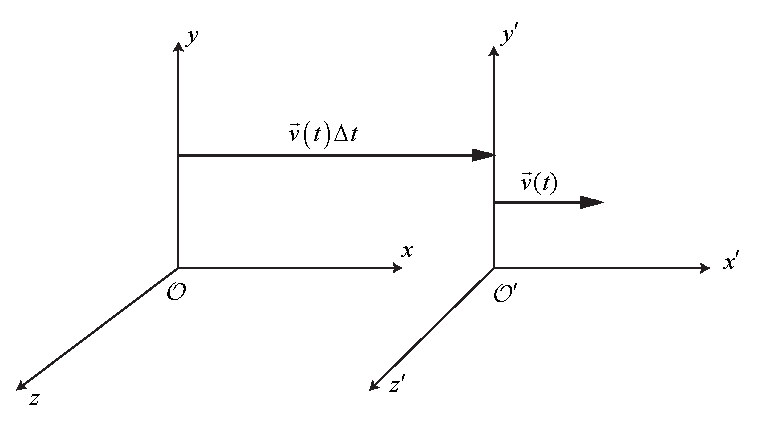
\includegraphics[width = 0.5\textwidth, width = 300pt, angle = 0, keepaspectratio]{figures/traslating_reference_frame.eps}
	\captionsetup{width=0.75\textwidth}		
	\caption{Inertial reference frames in relative motion along one axis.}
	\label{inertial_ref_frame}
\end{figure}
Cosider two inertial reference frames, a stationary “laboratory” reference frame $\mathcal{O}$ with coordinates $(x,y,z,t)$ and a moving reference frame $\mathcal{O'}$ with coordinates $(x',y',z',t')$. Frame $\mathcal{O'}$ moves with velocity $\vec{v}$ with respect to  $\mathcal{O}$ as shown in Figure~\ref{inertial_ref_frame}. Observers in $\mathcal{O}$ and $\mathcal{O'}$ measure different values for the electromagnetic fields. Rigorous comparison of these measurements can be made if one knows how fields transform from $\mathcal{O}$ to $\mathcal{O'}$ or vice versa. The transformation laws follow from the theory of special relativity. 

The basic postulates of special relativity are as follows:
\begin{enumerate}
	\item The law of physics are the same in all inertial reference frames.
	\item Observer in inertial reference frames measure the same value for the speed of light.
\end{enumerate}

The first postulate implies that the quasi-static field equations must have the same form in both  $\mathcal{O}$ and $\mathcal{O'}$ as shown in the following equations
\setlength{\columnseprule}{1pt}
\bigskip
\ \newline \centerline{\textbf{Quasi-Static Equations}}
\begin{multicols}{2}
	\centerline{\textbf{Reference frame $\mathcal{O}$}}	
	\begin{equation*}
		\begin{aligned}
			&\vec{\nabla}\times\vec{H} = \vec{J} \\[6pt]
			&\vec{\nabla}\cdot\vec{B} = 0 \\[6pt]
			&\vec{\nabla}\times\vec{E} = -\frac{\partial\vec{B}}{\partial t} \\[6pt]
			&\vec{\nabla}\cdot\vec{D} = \rho
		\end{aligned}
	\end{equation*} 
	\ \newline
	\columnbreak
	\ \newline
	\centerline{\textbf{Reference frame $\mathcal{O'}$}}	
\begin{equation}\label{maxwell_eq_moving_frame}
	\begin{aligned}
		&\vec{\nabla}'\times\vec{H}' = \vec{J}' \\[6pt]
		&\vec{\nabla}'\cdot\vec{B}' = 0 \\[6pt]
		&\vec{\nabla}'\times\vec{E}' = -\frac{\partial\vec{B}'}{\partial t} \\[6pt]
		&\vec{\nabla}'\cdot\vec{D}' = \rho'
	\end{aligned}
\end{equation} 
	\ \newline
\end{multicols}
Here $\vec{\nabla}'$ is the gradient operator with respect to the $(x',y',z',t')$ coordinate
\begin{equation*}
	\begin{aligned}
		&\vec{\nabla}'= \frac{\partial}{\partial x'}\vec{i}\,'+\frac{\partial}{\partial y'}\vec{j}\,'+\frac{\partial}{\partial z'}\vec{k}\,'
	\end{aligned}
\end{equation*} 
our goal is to determine the transformation laws for the field going from $\mathcal{O}$ to $\mathcal{O'}$ and vice versa. We can determine these if we know the transformation relations for the coordinate variables. These follow from the second postulate of the special relativity and are given by
 \begin{equation}\label{lorentz}
 	\begin{aligned}
 		&t'=\gamma\big(t-\beta x/c\big) \\[6pt]
 		&x'=\gamma\big(x-\beta ct\big) \\[6pt] 		
 		&y'=y \\[6pt]
		&z'=z
 	\end{aligned}
 \end{equation} 
where $$ \gamma=\frac{1}{\sqrt{1+\beta^2}} $$ and $$\beta=\frac{v}{c} $$. Here, $c$ is the speed of the light in a vacuum. We are interested in low-velocity electromechanical devices for which $u\ll c$. Therefore $$\beta\approx 0$$ and $$\gamma\approx 1$$.
Substituting the above approximations Eq.~\eqref{lorentz} reduce to the Galilean transform relation
  \begin{equation}\label{galileo}
 	\begin{aligned}
 		&t'=t \\[6pt]
 		&x'=x - vt \\[6pt] 		
 		&y'=y \\[6pt]
 		&z'=z
 	\end{aligned}
 \end{equation} 
This analysis generalized to the case of an arbitrary velocity as shown in Figure~\ref{inertial_ref_frame_space}.
\begin{figure}[H]
	\centering
	\includegraphics[width = 0.5\textwidth, width = 250pt, angle = 0, keepaspectratio]{figures/traslating_reference_frame_space.eps}
	\captionsetup{width=0.75\textwidth}		
	\caption{Inertial reference frames in relative motion.}
	\label{inertial_ref_frame_space}
\end{figure}
For this case we find that
  \begin{equation}\label{galileo_space}
	\begin{aligned}
		&t'=t \\[6pt]
		&x'=x - v_xt \\[6pt] 		
		&y'=y - v_yt \\[6pt] 		
		&z'=z - v_zt 	
	\end{aligned}
\end{equation} 
Now that we know the transform relations for the coordinates, we can determine the corresponding relations for the field equations. These will ultimately enable us to compare the fields in the two reference frames. We start by considering a scalar-valued function $f'$ of the \textbf{primed} coordinates, $f'\big(x',y',z'\big)$. By virtue of Eq.~\eqref{galileo_space}, $f'$ can be considered to be a function of the \textbf{unprimed} coordinates, $$f'\big(x',y',z'\big)=f'\big(x'\big(x,t\big),y'\big(y,t\big),z'\big(z,t\big)\big)$$.
We use the chain rule to determine the derivatives of $f'$ with respect to the \textbf{unprimed} coordinates. We consider spatial derivatives first and find that $$ \frac{\partial f'}{\partial x} =  \frac{\partial f'}{\partial x'} \frac{\partial x'}{\partial x} = \frac{\partial f'}{\partial x'}$$.
It follows that $$ \vec{\nabla}f'=\vec{\nabla}'f'$$.
Next, we consider the time derivative. From the chain rule we have 
  \begin{equation}
	\begin{aligned}
		\frac{\partial f'}{\partial t} &= \frac{\partial f'}{\partial t'}\,\frac{\partial t'}{\partial t}\,+\,\frac{\partial f'}{\partial x'}\,\frac{\partial x'}{\partial t}\,+\,\frac{\partial f'}{\partial y'}\,\frac{\partial y'}{\partial t}\,+\,\frac{\partial f'}{\partial z'}\,\frac{\partial z'}{\partial t} = \\[8pt]
		& = \frac{\partial f'}{\partial t}\,-\,\frac{\partial f'}{\partial x'} v_x\,-\,\frac{\partial f'}{\partial y'} v_y\,-\,\frac{\partial f'}{\partial z'} v_z
	\end{aligned}
\end{equation} 
This can be rewritten as 
  \begin{equation}\label{movref1}
	\begin{aligned}
		\frac{\partial f'}{\partial t} &= \frac{\partial f'}{\partial t'}\,-\,\vec{v}\cdot\big(\vec{\nabla}'f'\big)
	\end{aligned}
\end{equation} 
or
  \begin{equation}\label{movref2}
	\begin{aligned}
		\frac{\partial f'}{\partial t'} &= \frac{\partial f'}{\partial t}\,+\,\vec{v}\cdot\big(\vec{\nabla}f'\big)
	\end{aligned}
\end{equation} 
The relations \ref{movref1} and \ref{movref2} relate the derivatives in $\mathcal{O}$ and in $\mathcal{O'}$ for scalar-valued function. A similar analysis applies to vector-valued function. Let $\vec{A}'\big(x',y',z',t'\big)$ be a vector-valued function of the \textbf{primed} coordinate variables. This can also be considered to be a vector-valued function of the \textbf{unprimed} coordinates
\begin{equation*}
	\begin{aligned}
		\vec{A}\,'\big(x',y',z',t'\big) = 	\vec{A}\,'\big(x'\big(x,t\big),y'\big(y,t\big),z'\big(z,t\big)\big)
	\end{aligned}
\end{equation*} 
It is easy to check that
\begin{equation}\label{ident1}
	\begin{aligned}
		\vec{\nabla}'\cdot\vec{A}\,' = \vec{\nabla}\cdot\vec{A}\,'
	\end{aligned}
\end{equation} 
and that
\begin{equation}\label{ident2}
	\begin{aligned}
		\vec{\nabla}'\times\vec{A}\,' = \vec{\nabla}\times\vec{A}\,'.
	\end{aligned}
\end{equation} 
Similarly, by taking the time derivative we find that
\begin{equation}
	\begin{aligned}
		\frac{\partial \vec{A}\,'}{\partial t'} = \frac{\partial \vec{A}\,'}{\partial t} + \big(\vec{v}\cdot\vec{\nabla}\big)\vec{A}\,'.
	\end{aligned}
\end{equation} 
This can be rewritten as
  \begin{equation}\label{ident3}
  	\begin{aligned}
  		\frac{\partial \vec{A}\,'}{\partial t'} = \frac{\partial \vec{A}\,'}{\partial t} + \vec{v}\big(\vec{\nabla}\cdot\vec{A}\,'\big)-\vec{\nabla}\times\big(\vec{v}\times\vec{A}\,'\big),
  	\end{aligned}
  \end{equation} 
where we have used the identity $\vec{\nabla}\times\big(\vec{A}\times\vec{B}\big)=\big(\vec{B}\cdot\vec{\nabla}\big)\vec{A}-\big(\vec{A}\cdot\vec{\nabla}\big)\vec{B}$. Finally, substitute Eqs.~\eqref{ident1}, \ref{ident2} and \ref{ident3} into the quasi-static equations for $\mathcal{O}'$ in \ref{maxwell_eq_moving_frame} we obtain 
\begin{equation}\label{maxwell_mov1}
	\begin{aligned}
		&\vec{\nabla}\times\vec{H}\,'=\vec{J}\,' \\[8pt]
		&\vec{\nabla}\cdot\vec{B}\,'= 0 \\[8pt]
		&\vec{\nabla}\times\big(\vec{E}\,'-\vec{u}\times\vec{B}\,'\big)=-\frac{\partial\vec{B}\,'}{\partial t} \\[8pt]
		&\vec{\nabla}\cdot\vec{J}\,'=0
	\end{aligned}
\end{equation} 
We have used $\vec{\nabla}\cdot\vec{B}\,'=0$ in the third equation of Eq.~\eqref{maxwell_mov1}. By comparing Eqs.~\eqref{maxwell_eq_moving_frame} and Eq.~\eqref{maxwell_mov1} we find that the fields transform as follows:
\bigskip \ \newline	\centerline{\textbf{Transformation Relations}}
\begin{equation}\label{TR1}
	\begin{aligned}
		&\vec{H}\,'=\vec{H}
	\end{aligned}
\end{equation} 
\begin{equation}\label{TR2}
	\begin{aligned}
		&\vec{B}\,'=\vec{B}
	\end{aligned}
\end{equation} 
\begin{equation}\label{TR3}
	\begin{aligned}
		&\vec{E}\,'=\vec{E}+\vec{v}\times\vec{B}
	\end{aligned}
\end{equation} 
\begin{equation}\label{TR4}
	\begin{aligned}
		&\vec{J}\,'=\vec{J}
	\end{aligned}
\end{equation} 
In Eqs.~\eqref{TR1}-~\ref{TR4} the variables $\big(\vec{H},\vec{B},\vec{E},\vec{u},\vec{J}\big)$ are measured in the stationary reference frame $\mathcal{O}$ and the variables $\big(\vec{H}\,',\vec{B}\,',\vec{E}\,',\vec{J}\,'\big)$ are measured in the moving frame $\mathcal{O}'$. For these relations to hold, the variables must be compared \textbf{at the same physical point in space}. For example, from Eqs.~\eqref{galileo_space} and \ref{TR3} we have
\begin{equation*}
	\begin{aligned}
		\vec{E}\,'\big(x',y',z',t'\big)= & \vec{E}\big(x-v_xt,y-v_yt,z-v_zt,t\big) \\[8pt]
		&+ \vec{v}\times\vec{B}\big(x-v_xt,y-v_yt,z-v_zt,t\big).
	\end{aligned}
\end{equation*} 
Notice that we have assumed that $\vec{v}$ is a constant (independent of position). 

The relations \ref{TR1}-~\ref{TR4} give the transformations for the fields and the source. However, we still need to know the constitutive relations in $\mathcal{O}$ and $\mathcal{O'}$. We apply a general principle that says that the constitutive relations form moving media are the same as for stationary media when they are written in term of the fields defined in an inertial reference frame moving with the media. For example for a linear, homogeneous and isotropic media at rest in $\mathcal{O'}$ we have $\vec{J}\,' = \sigma\vec{E}\,'$ and $\vec{B}'=\mu\vec{H}\,'$. However, in $\mathcal{O}$ (which is moving with respect to the media) the relations are modified by virtue of Eqs.~\eqref{TR1}-~\ref{TR4}. Specifically, we find that
\setlength{\columnseprule}{1pt}
\bigskip
\ \newline \centerline{\textbf{Constitutive Relations}}
\begin{multicols}{2}
	\centerline{\textbf{Reference frame $\mathcal{O}$}}	
	\begin{equation*}
		\begin{aligned}
			&\vec{J} =  \sigma\big(\vec{E}+\vec{v}\times\vec{B}\big) \\[8pt]
			&\vec{B} =  \mu\vec{H}
		\end{aligned}
	\end{equation*} 
	\ \newline
	\columnbreak
	\ \newline
	\centerline{\textbf{Reference frame $\mathcal{O'}$}}	
	\begin{equation}
		\begin{aligned}
			&\vec{J}\,' =  \sigma\vec{E}\,' \\[8pt]
			&\vec{B}\,' =  \mu\vec{H}\,'
		\end{aligned}
	\end{equation} 
	\ \newline
\end{multicols}
In our study of electromechanical devices we will need to determine the voltage induced in a coil as it moves through a stationary magnetic field. Therefore, we discuss this in some detail. Consider a reference frame $\mathcal{O}$ in which there is a static (but not necessarily uniform) $\vec{B}$-field. Consider an open conductor moving with velocity $\vec{v}$ relative to $\mathcal{O}$. Assume that the conductor has a conductivity $\sigma$ (as measured by observers in both $\mathcal{O}$ and $\mathcal{O}'$). We want to determine the voltage induced across the terminals of the conductor as measured in $\mathcal{O}$. We apply Faraday's Law to a stationary contour $C$ that passes through the conductor at a given (but arbitrary) instant in time,
 \begin{equation}\label{faraday_ex}
 	\begin{aligned}
 		&\oint_C \vec{E}\cdot\,d\vec{l}=-\frac{d}{d t}\int_S\vec{B}\cdot d\vec{a}
 	\end{aligned}
 \end{equation} 
We label the terminals $a$ and $b$, and then decompose the left-hand side of Eq.~\eqref{faraday_ex} into integrals across the terminals and the conductor itself,
 \begin{equation}\label{faraday_path_int}
	\begin{aligned}
		\oint_C \vec{E}\cdot\,d\vec{l}&=\underbrace{\int_{b}^{a}\vec{E}\cdot d\vec{l}}_{\text{terminals}}\,+\,\underbrace{\int_{a}^{b}\vec{E}\cdot d\vec{l}}_{\text{conductor}} \\[8pt]
		&=-u+\underbrace{\int_{a}^{b}\vec{E}\cdot d\vec{l}}_{\text{conductor}}
	\end{aligned}
\end{equation}  
where $u$ is the terminal voltage (as measured in $\mathcal{O}$). As for the remaining integral, from Eqs.~\eqref{TR3}-~\ref{TR3} we have $\vec{E} = \vec{E}\,'-\vec{u}\times\vec{B}$ and $\vec{E}\,' = \vec{J}\,'/\sigma = \vec{J}/\sigma$. Therefore
 \begin{equation}\label{moving_conductor}
	\begin{aligned}
		\vec{E}=\frac{\vec{J}}{\sigma}-\vec{v}\times\vec{B}\qquad\text{moving conductor}
	\end{aligned}
\end{equation} 
Notice that all the terms in Eq.~\eqref{moving_conductor} are measured in $\mathcal{O}$ (the conductor is moving with respect to $\mathcal{O}$). As the conductor is open, there is no current flowing through it ($\vec{J}=\vec{0}$) and, therefore,
 \begin{equation}\label{moving_conductor2}
	\begin{aligned}
		\vec{E}=-\vec{v}\times\vec{B}
	\end{aligned}
\end{equation} 
Combining Eqs.~\eqref{faraday_ex}, \ref{faraday_path_int} and \ref{moving_conductor2} gives us
 \begin{equation}\label{faraday_3}
	\begin{aligned}
		u=-\int_{a}^{b}\big(\vec{v}\times\vec{B}\big)\cdot d\vec{l} + \frac{d}{d t}\int_S\vec{B}\cdot d\vec{a}.
	\end{aligned}
\end{equation} 
Because $\vec{B}$, $C$, $S$ and $d\vec{a}$ are constant in $\mathcal{O}$, the last term in Eq.~\eqref{faraday_3} is zero and the terminal voltage reduces to 
 \begin{equation}\label{faraday_4}
	\begin{aligned}
		u=-\int_{a}^{b}\big(\vec{v}\times\vec{B}\big)\cdot d\vec{l}.
	\end{aligned}
\end{equation} 
It is important to note that if there were a time varying current in the conductor, the flux through the circuit due to the current would add to the voltage via last term in Eq.~\eqref{faraday_3}.
\begin{example}
A conductive bar is in sliding contact with a pair of stationary conducting rails as shown in Figure~\ref{moving_coil_1}. The bar is moving through a constant uniform $\vec{B}$-field with a constant velocity $v$ relative to the rails. Assuming the bar and rails are ideal conductor, we determine the voltage across the rails.

We choose a reference frame $\mathcal{O}$ at rest with respect to the rails and a stationary contour $C$ (dotted line) that runs clockwise through the rails and passes through the bar \textbf{at a single instant in time}. Apply Faraday's law to $C$
 \begin{equation}\label{ex_eq_1}
	\begin{aligned}
		\oint_C \vec{E}\cdot d\vec{l} = - \frac{d}{dt} \int_S\vec{B}\cdot d\vec{a}.
	\end{aligned}
\end{equation} 
As $\vec{B}$, $C$, $S$ and $d\vec{a}$ are constant in $\mathcal{O}$ we have
 \begin{equation}\label{}
	\begin{aligned}
	\frac{d}{dt} \int_S\vec{B}\cdot d\vec{a} = 0
	\end{aligned}
\end{equation} 
\begin{figure}[H]
	\centering
	\includegraphics[width = 0.5\textwidth, width = 250pt, angle = 0, keepaspectratio]{figures/moving_coil_1.eps}
	\captionsetup{width=0.75\textwidth}		
	\caption{Conductive bar moving along conductive rails.}
	\label{moving_coil_1}
\end{figure}
Substitute this into Eq.~\eqref{ex_eq_1} and decompose the right-hand side into integrals over the various segment and obtain,
\begin{equation}\label{}
	\begin{aligned}
		\underbrace{\int_{(-)}^{(+)}\vec{E}\cdot\,d\vec{l}}_{\text{terminals}} \, + \underbrace{\int\vec{E}\cdot\,d\vec{l}}_{\text{upper rail}} \, + 
		\underbrace{\int\vec{E}\cdot\,d\vec{l}}_{\text{moving bar}} \, + 
		\underbrace{\int\vec{E}\cdot\,d\vec{l}}_{\text{lower rail}} = 0
	\end{aligned}
\end{equation} 
As the upper and lower rails are ideal conductor ($\sigma \approx \infty$) we have $E_{rail} \approx 0$ and, therefore, 
\begin{equation}\label{}
	\begin{aligned}
		\underbrace{\int\vec{E}\cdot\,d\vec{l}}_{\text{moving bar}} \, = 
		\underbrace{\int\vec{E}\cdot\,d\vec{l}}_{\text{lower rail}} = 0
	\end{aligned}
\end{equation} 
In the moving bar we have 
\begin{equation*}\label{}
	\begin{aligned}
		\underbrace{\int\vec{E}\cdot\,d\vec{l}}_{\text{moving bar}} \, = 
		\int\Big(\vec{E}\,'-\vec{v}\times\vec{B}\Big)\cdot d\vec{l}
	\end{aligned}
\end{equation*} 
But $\vec{E}\,'=\vec{J}\,'/\sigma = \vec{J}/\sigma$ and, therefore, 
\begin{equation}\label{voltage_moving_bar}
	\begin{aligned}
		\underbrace{\int\vec{E}\cdot\,d\vec{l}}_{\text{moving bar}} \, = 
		-\int\Big(\vec{v}\times\vec{B}\Big)\cdot d\vec{l}
	\end{aligned}
\end{equation} 
To evaluate the Eq.~\eqref{voltage_moving_bar} we use $\vec{v} = v\vec{i}$, $\vec{B} = B\vec{k}$ and $d\vec{l}=dy\vec{j}$.
Therefore 
\begin{equation*}\label{}
	\begin{aligned} 
		\underbrace{\int\vec{E}\cdot\,d\vec{l}}_{\text{moving bar}} \, = -\int\Big(\vec{v}\times\vec{B}\Big)\cdot d\vec{l} = -\int_{h}^{0}(-vB)dy=-vBh
	\end{aligned}
\end{equation*} 
Hence the terminal voltage results in following equation
\begin{equation}\label{}
	\begin{aligned}
		u = \int_{(-)}^{(+)}\vec{E}\cdot\,d\vec{l} = vBh
	\end{aligned}
\end{equation} 
\end{example}

\section{Electrical equations}
The electrical equations for an electromechanical device follow from circuit theory, which in turn is based on quasi-static field theory. In this section, we derive a generalized version of Kirchhoff's voltage law that takes into account the effects of electromagnetic coupling.

We study two different types of circuits, stationary and moving coil. In a stationery circuit, all the circuit components are at rest with respect to one another. For these circuits, we apply quasi-static field theory in a reference frame fixed with respect to the circuit. The electromechanical coupling is accounted for by a flux linkage term that takes into account the voltage induced in the circuit by a time rate of change of magnetic flux through it. This change in flux is due to a change in the magnetic field that can be caused by a change in the current and/or by the movement of a ferromagnetic member that alters the field. Mechanical motion is taken into account by considering the flux to be a function of both the circuit current and mechanical displacement.

In a moving coil circuit, a coil is moving with respect to an external magnetic field. To analyze this kind of circuit, we apply quasi-static field theory in a reference frame that is rest with respect to the magnetic field. Mechanical motion is taken into account by the voltage induced in the coil as it moves through the field. Finally, it is important to note that the following analysis applies to magnetically linear devices.
\subsection{Stationary circuits}
In this section we study electromechanical devices with stationary electrical circuit. Such a device is shown in Figure~\ref{elect_mech_actuator}. It consists of a voltage source $u$, a resistor $R$ and a magnetic circuit with a fixed coil and a moving soft magnetic bar that alters the flux through the coil when it moves. We analyze the electrical circuit using quasi-static field theory. Specifically, we choose a reference frame at rest with respect to the circuit and a fixed integration contour $C$ along the circuit. At any point along the circuit the electrical field is given by 
\begin{equation}\label{electrical_field_source}
	\begin{aligned}
		\vec{E} = -\frac{\partial \vec{A}}{\partial t} - \vec{\nabla}\varphi
	\end{aligned}
\end{equation} 
where $-\vec{\nabla}\varphi$ is due to the accumulation of the charge along the circuit, and $\partial \vec{A}/\partial t$ is due to the time-varying current. We evaluate the line integral of Eq.~\eqref{electrical_field_source} clockwise along $C$ and obtain
\begin{equation*}\label{}
	\begin{aligned}
		\oint_{C} \vec{E}\cdot d\vec{l} = -\oint_{C} \frac{\partial \vec{A}}{\partial t}\cdot d\vec{l} - \oint_{C}\vec{\nabla}\varphi\cdot d\vec{l}.
	\end{aligned}
\end{equation*} 
The first term can be decomposed into integrals over the individual components
\begin{equation}\label{faraday_path}
	\begin{aligned}
		\underbrace{\int_{(-)}^{(+)}\vec{E}\cdot\,d\vec{l}}_{\text{source}} \, + \underbrace{\int\vec{E}\cdot\,d\vec{l}}_{\text{resistor}} \, + 
		\underbrace{\int\vec{E}\cdot\,d\vec{l}}_{\text{coil}} = -\oint_{C} \frac{\partial \vec{A}}{\partial t}\cdot d\vec{l} - \oint_{C}\vec{\nabla}\varphi\cdot d\vec{l}.
	\end{aligned}
\end{equation} 
Notice that $$\oint_{C}\vec{\nabla}\varphi\cdot d\vec{l}$$ because it entails the integration of a conservative vector field $\vec{\nabla}\varphi$ around a closed path. Also notice that although $$\oint_{C} \frac{\partial \vec{A}}{\partial t}\cdot d\vec{l}$$ is evaluated around the entire path, the major contribution to it is from inductor.
\begin{figure}[H]
	\centering
	\includegraphics[width = 0.5\textwidth, width = 250pt, angle = 0, keepaspectratio]{figures/generic_electromecanical_actuator.eps}
	\captionsetup{width=0.75\textwidth}		
	\caption{Electromechanical actuator circuit.}
	\label{elect_mech_actuator}
\end{figure}
We assume that the source is ideal with no internal resistance and define the voltage impressed at the terminal in the usual way:
\begin{equation}\label{faraday_path_1}
	\begin{aligned}
		u=\int_{(-)}^{(+)}\vec{E}\cdot\,d\vec{l}
	\end{aligned}
\end{equation} 
Thus, Eq.~\eqref{faraday_path} becomes 
\begin{equation}\label{faraday_path_2}
	\begin{aligned}
		u= \underbrace{\int\vec{E}\cdot\,d\vec{l}}_{\text{resistor}} \, + \,
		\underbrace{\int\vec{E}\cdot\,d\vec{l}}_{\text{coil}}\, + \, \oint_{C} \frac{\partial \vec{A}}{\partial t}\cdot d\vec{l}.
	\end{aligned}
\end{equation} 
In the resistor $\vec{J}=\sigma\vec{E}$ (Ohm's law). Therefore,
\begin{equation}\label{faraday_path_3}
	\begin{aligned}
		&\underbrace{\int\vec{E}\cdot\,d\vec{l}}_{\text{resistor}}  = \underbrace{\int\frac{\vec{J}}{\sigma}\cdot\,d\vec{l}}_{\text{resistor}} = i R \\[8pt]
		&\underbrace{\int\vec{E}\cdot\,d\vec{l}}_{\text{coil}}= i R_{coil}
	\end{aligned}
\end{equation} 
which results in
\begin{equation}\label{vector_pot_1}
	\begin{aligned}
		u = i\big(R+R_{coil}\big)\, + \, \oint_{C} \frac{\partial \vec{A}}{\partial t}\cdot d\vec{l}.
	\end{aligned}
\end{equation} 
Now consider the last term in Eq.~\eqref{vector_pot_1}. We can rewrite this as follows:
 \begin{equation}\label{vector_pot_2}
 	\begin{aligned}
 		\oint_{C} \frac{\partial \vec{A}}{\partial t}\cdot d\vec{l} &= \int_S\Big(\vec{\nabla}\times\frac{\partial \vec{A}}{\partial t}\Big)\cdot d\vec{a} \\[8pt]
 		&=\int_S\frac{\partial \vec{B}}{\partial t}\cdot d\vec{a} \\[8pt]
 		&=\frac{d}{dt}\int_S\vec{B}\cdot d\vec{a} \\[8pt]
 		&= \frac{d\psi}{dt}
 	\end{aligned}
 \end{equation} 
where $$\psi = \int_S\vec{B}\cdot d\vec{a} \qquad\text{(flux linkage).}$$
The symbol $\psi$ denotes the flux linkage, that is the total flux through (linking) the circuit. To determine $\psi$ we need to evaluate $$\int_S\vec{B}\cdot d\vec{a}$$ over an area bounded by the circuit path in accordance with Stokes's theorem. However, this integral can be difficult to evaluate depending on the topology of the circuit. For a simple single-turn current loop, the flux is denoted by $\phi$ and, therefore, $\psi=\phi$. For a tightly wound $N$ turn coil the flux linkage is $$\psi=N\phi\qquad\text{(N turn coil)}$$
where $phi$ is the flux through each turn.

We digress briefly to discuss the second and third step in Eq.~\eqref{vector_pot_2}. Notice that we have replaced the partial time derivative inside the integral by a total time derivative outside the integral. We do this because inside the integral, $\vec{B}$ is a function of both time-independent coordinate variables and other time-dependent variables (including $t$ itself). However, the integration effectively eliminates the time-independent variables, and leaves only the time-dependent variables. Therefore, the total time derivative is appropriate outside the integral. 

We return to the derivation. Substitute Eq.~\eqref{vector_pot_2} into Eq.~\eqref{vector_pot_1} and obtain
 \begin{equation}\label{vector_pot_3}
	\begin{aligned}
		u = i\big(R+R_{coil}\big)\, + \, \frac{d \psi}{d t}
	\end{aligned}
\end{equation} 
This is a generalization of Kirchhoff's voltage law. The term $\frac{d \psi}{d t}$ requires some discussion because it is key to the electromechanical coupling. This term represents the voltage induced in the circuit by a time rate of change of magnetic flux through the circuit. The change in flux can be due to a change in circuit current and/or to movement of a ferromagnetic member that alters the field. To account for this we write $\psi$ as a function of both the circuit current and the position of the member. Let $x$ and $\theta$ denote the position of the member when it executes linear and rotational motion, respectively. Then
 \begin{equation*}\label{}
	\psi = \left\lbrace 
	\begin{aligned}
		&\psi(i,x)\qquad\text{(linear motion)} \\[8pt]
		&\psi(i,\theta)\qquad\text{(rotational motion)} 
	\end{aligned}\right. 
\end{equation*}
Given this functional dependence, the total time derivative of $\psi$ is
 \begin{equation*}\label{}
	\frac{d\psi }{dt} = \left\lbrace 
	\begin{aligned}
		&\frac{\partial \psi(i,x)}{\partial i}\frac{d i}{d t} + \frac{\partial \psi(i,x)}{\partial x}\frac{d x}{d t} \qquad\text{(linear motion)} \\[8pt]
		&\frac{\partial \psi(i,\theta)}{\partial i}\frac{d i}{d t} + \frac{\partial \psi(i,\theta)}{\partial \theta}\frac{d \theta}{d t} \qquad\text{(rotational motion)} \\[8pt]
	\end{aligned}\right. 
\end{equation*}
or 
 \begin{equation}\label{}
	\frac{d\psi }{dt} = \left\lbrace 
	\begin{aligned}
		&L\frac{d i}{d t} + \frac{\partial \psi(i,x)}{\partial x}v \qquad\text{(linear motion)} \\[8pt]
		&L\frac{d i}{d t} + \frac{\partial \psi(i,\theta)}{\partial \theta}\omega \qquad\text{(rotational motion)} \\[8pt]
	\end{aligned}\right. 
\end{equation}
where $L$ is the inductance and which is defined by
 \begin{equation}\label{inductance_calc}
	\begin{aligned}
		L = \frac{\partial \psi}{\partial i}\qquad\text{inductance}
	\end{aligned}
\end{equation}
The variable $v=dx/dt$ and $\omega=d\theta/dt$ are the linear and angular velocities, respectively. It is important to note that the definition of inductance Eq.~\eqref{inductance_calc} applies only to magnetically linear devices. There is no simple definition of $L$ for nonlinear devices.

Finally, we obtain the following representations
 \begin{equation}\label{}
	\text{Electrical Equatios}\Rightarrow\left\lbrace 
	\begin{aligned}
		&u(t) = i(t)\big(R+R_{coil}\big) + L\frac{d i}{d t} + \frac{\partial \psi(i,x)}{\partial x}v  \quad\text{(linear m.)} \\[8pt]
		&u(t) = i(t)\big(R+R_{coil}\big) + L\frac{d i}{d t} + \frac{\partial \psi(i,\theta)}{\partial \theta}\omega \quad\text{(rotational m.)}
	\end{aligned}\right. 
\end{equation}
These are the electrical equations of motion for stationary circuits with time varying currents and moving ferromagnetic member.

\subsection{Moving coils}
In this section we derive Kirchhoff's voltage law for circuit that have a coil moving through an external field $\vec{B_M}$. All the other circuit are stationary with respect to the field. Let $\mathcal{O}$ denote the stationary reference frame. The coil moves with velocity $\vec{v}$ through $\vec{B}_M$, which is constant (but not necessary uniform) with respect to $\mathcal{O}$. 
\begin{figure}[H]
	\centering
	\includegraphics[width = 0.5\textwidth, width = 300pt, angle = 0, keepaspectratio]{figures/moving_coil_3.eps}
	\captionsetup{width=0.75\textwidth}		
	\caption{Moving conductor actuator.}
	\label{moving_coil_3}
\end{figure}
Such a circuit is shown in Figure~\ref{moving_coil_3}. This figure shows a linear actuator consisting of a conductive bar of mass $m$ in sliding contact with a pair of stationary conductive rails. The rails are connected to a voltage source $u$ and a resistor $R$ that limits the current. The bar is moving through a constant uniform $\vec{B}$-field with a time-dependent velocity $v(t)$ relative to the rails. 

We derive Kirchhoff's voltage law for a circuit with a moving coil by applying Faraday's law to a stationary contour $C$ that passes through the circuit and coincides with the coil for a given position of its travel (the dotted line in Figure~\ref{moving_coil_3}). Thus, $C$ coincides with the entire circuit at a single instant in time. We evaluate
 \begin{equation}\label{faraday_mc_1}
	\begin{aligned}
		&\oint_C \vec{E}\cdot\,d\vec{l}=-\frac{d}{d t}\int_S\vec{B}\cdot d\vec{a}
	\end{aligned}
\end{equation} 
clockwise around the contour and obtain 
\begin{equation}\label{faraday_path_4}
	\begin{aligned}
		\underbrace{\int_{(-)}^{(+)}\vec{E}\cdot\,d\vec{l}}_{\text{source}} \, + \underbrace{\int\vec{E}\cdot\,d\vec{l}}_{\text{resistor}} \, + 
		\underbrace{\int\vec{E}\cdot\,d\vec{l}}_{\text{coil}} = - \frac{d}{dt}\int_S\vec{B}\cdot d\vec{a} .
	\end{aligned}
\end{equation} 
The integrals over the fixed components (source and resistor) follow from Eqs.~\eqref{faraday_path_1}-\ref{faraday_path_3}. We obtain
 \begin{equation}\label{faraday_path_5}
	\begin{aligned}
		u = iR+\int_{\text{coil}}\vec{E}\cdot d\vec{l} + \frac{d}{dt}\int_S\vec{B}\cdot d\vec{a}
	\end{aligned}
\end{equation} 
The coil is moving with velocity $v$ through $\vec{B}_M$. The $\vec{E}$-field in it as measured in $\mathcal{O}$ is given by
\begin{equation}\label{faraday_path_6}
	\begin{aligned}
		\vec{E}=\frac{\vec{J}}{\sigma} - \vec{v}\times\vec{B}_M.
	\end{aligned}
\end{equation} 
Therefore,
\begin{equation}\label{faraday_path_7}
	\begin{aligned}
		\int_{\text{coil}}\vec{E}\cdot d\vec{l}&=\int_{\text{coil}}\Big(\frac{\vec{J}}{\sigma}-\vec{v}\times\vec{B}_M\Big)\cdot d\vec{l} \\[8pt]
		&=iR_{\text{coil}} - \int_{\text{coil}}\big(\vec{v}\times\vec{B}_M\big)\cdot d\vec{l}
	\end{aligned}
\end{equation} 
where $R_{coil}$ is the resistance of the coil. Substitute Eq.~\eqref{faraday_path_7} into Eq.~\eqref{faraday_path_5} and obtain
 \begin{equation}\label{faraday_path_8}
	\begin{aligned}
		u(t) = i(t)\big(R+R_{\text{coil}}\big)-\int_{\text{coil}}\big(\vec{v}\times\vec{B}_M\big)\cdot d\vec{l} + \frac{d}{dt}\int_S\vec{B}\cdot d\vec{a}
	\end{aligned}
\end{equation} 
Now consider the last term in Eq.~\eqref{faraday_path_8}. The dominant contribution to this term comes from the coil. Moreover, as the system is magnetically linear we can write $\vec{B}$ as a superposition of two fields: the $\vec{B}_i$ due to the current $i$ and the external field $\vec{B}_M$, $$ \vec{B}=\vec{B}_i+\vec{B}_M$$. Therefore, the last term in Eq.~\eqref{faraday_path_8} can be rewritten as
 \begin{equation}\label{faraday_path_9}
	\begin{aligned}
		\frac{d}{dt}\int_S\vec{B}\cdot d\vec{a} &= \frac{d}{dt}\int_{\text{coil}}\vec{B}_i\cdot d\vec{a} + \frac{d}{dt}\int_{\text{coil}}\vec{B}_M\cdot d\vec{a}  \\[8pt]
		&= \frac{d}{dt} \psi_{\text{coil}}(i) + \frac{d}{dt}\int_{\text{coil}}\vec{B}_M\cdot d\vec{a} \\[8pt]
		&= L\frac{di}{dt} + \frac{d}{dt}\int_{\text{coil}}\vec{B}_M\cdot d\vec{a}
	\end{aligned}
\end{equation} 
where $$\psi_{\text{coil}}(i)=\int_{\text{coil}}\vec{B}_i\cdot d\vec{a}$$ and we have used the definition of inductance $$L=\frac{d}{di} \psi_{\text{coil}}(i)$$
Finally, we substitute Eq.~\eqref{faraday_path_9} into Eq.~\eqref{faraday_path_8} and find that
 \begin{equation}\label{faraday_path_10}
	\begin{aligned}
		u(t) = i(t)\big(R+R_{\text{coil}}\big)+L\frac{di}{dt}-\int_{\text{coil}}\big(\vec{v}\times\vec{B}_M\big)\cdot d\vec{l} + \frac{d}{dt}\int_{\text{coil}}\vec{B}_M\cdot d\vec{a}
	\end{aligned}
\end{equation} 
This is a generalization of Kirchhoff's voltage law that takes into account the voltage induced in a coil as it moves through $\vec{B}_M$. If $\vec{B}_M$ is static, $$\frac{d}{dt}\int_{\text{coil}}\vec{B}_M\cdot d\vec{a}=0$$ and Eq.~\eqref{faraday_path_10} reduces to 
  \begin{equation}\label{faraday_path_11}
 	\begin{aligned}
 		u = i\big(R+R_{\text{coil}}\big)+L\frac{di}{dt}-\int_{\text{coil}}\big(\vec{v}\times\vec{B}_M\big)\cdot d\vec{l}
 	\end{aligned}
 \end{equation} 
It is important to note that the line integral in Eq.~\eqref{faraday_path_11} is evaluated with the direction of integration in the same direction of the current.

The voltage equation~\ref{faraday_path_11} applies to a coil in linear motion, however, it can be generalized to the case of coil that is rotating. Specifically, if a segment $dl$ of the coil is rotating with an angular velocity $\omega$ at a distance $\vec{r}$ with respect to a fixed reference frame, then its linear velocity is
  \begin{equation}\label{rotational}
	\begin{aligned}
		\vec{v}=\vec{\omega}\times\vec{r}
	\end{aligned}
\end{equation} 
We substitute Eq.~\eqref{rotational} into Eq.~\eqref{faraday_path_11} and obtain the circuit equation for rotational motion.
   \begin{equation}\label{faraday_path_12}
 	\begin{aligned}
 		u(t) = i(t)\big(R+R_{\text{coil}}\big)+L\frac{di}{dt}-\int_{\text{coil}}\Big[\big(\vec{\omega}\times\vec{r}\,\big)\times\vec{B}_M\Big]\cdot d\vec{l}
 	\end{aligned}
 \end{equation} 
It is important to note that when evaluating Eq.~\eqref{faraday_path_12} the velocity $\big(\vec{\omega}\times\vec{r}\,\big)$ must be evaluated before the cross product with $\vec{B}_M$ is taken. If the rotation is with respect to a specific axis (which we label the $z$-axis), then $\vec{\omega}=\omega\vec{k}$ and Eq.~\eqref{faraday_path_12} can be rewritten as
   \begin{equation}\label{faraday_path_13}
	\begin{aligned}
		u(t) = i(t)\big(R+R_{\text{coil}}\big)+L\frac{di}{dt}-\int_{\text{coil}}\Big[\big(\vec{\omega}\times\vec{r}_{\perp }\,\big)\times\vec{B}_M\Big]\cdot d\vec{l}
	\end{aligned}
\end{equation} 
where $\vec{r}_{\perp}$ is a vector from (and perpendicular to) the $z$-axis to the segment $l\vec{l}$.

\section{Energy analysis}
In this section we discuss an energy method for the analysis of electromechanical devices. This method, based on the conservation of energy, is used to determine the force or torque on a moving member. It is especially useful for the analysis of magnetic circuit actuators as we shall see.

We start with the basic energy balance relation shown in Figure~\ref{EBR_1}:
\begin{figure}[H]
	\centering
	\includegraphics[width = 0.5\textwidth, width = 400pt, angle = 0, keepaspectratio]{figures/energy_balance.eps}
	\captionsetup{width=0.75\textwidth}		
	\caption{Energy balance relation.}
	\label{EBR_1}
\end{figure}
Apply this to a system that is subjected to an infinitesimal (virtual) displacement and obtain
   \begin{equation}\label{EBR_2}
	\begin{aligned}
		\underbrace{dW_e}_{\substack{\text{electrical} \\ \text{energy input}}}  = \,
		\underbrace{dW_{\text{loss}}}_{\substack{\text{energy} \\ \text{dissipated}}} \, + \,
		\underbrace{dW_{\text{fld}}}_{\substack{\text{stored} \\ \text{field energy}}} \, + \,
		\underbrace{dW_{\text{mech}}}_{\substack{\text{mechanical} \\ \text{energy}}}
	\end{aligned}
\end{equation} 
The term $dW_{\text{loss}}$ accounts for energy dissipation due to loss mechanisms such as ohmic heating and mechanical friction. For our purposes, we consider the system to be lossless and treat the loss mechanisms as external to the system. For example, a real inductor can be treated as a lossless coil in series with an external resistance. Thus, without loss of generality, we restrict our attention to lossless systems in which $dW_{\text{loss}}=0$. For these systems energy balance equation~\ref{EBR_2} becomes
   \begin{equation}\label{EBR_3}
	\begin{aligned}
		{dW_e}  = \,
		{dW_{\text{fld}}} \, + \,
		{dW_{\text{mech}}}
	\end{aligned}
\end{equation} 
We consider the various terms in Eq.~\eqref{EBR_3}. Recall that mechanical motion couples to the electrical equations via flux linkage $\psi$. Moreover, the voltage $e$ induced across the terminals of an electromechanical component such as coil is $e=d\psi/dt$. Therefore, the electrical energy input into the terminals of the component during a time $dt$ is
\begin{equation}\label{EBR_4}
	\begin{aligned}
		{dW_e}  &= \frac{d\psi}{dt}i\,dt \\[8pt]
			&=d\psi i
	\end{aligned}
\end{equation} 
Substitute Eq.~\eqref{EBR_4} into Eq.~\eqref{EBR_3} and obtain
\begin{equation}\label{EBR_5}
	\begin{aligned}
		dW_{fld}  &= d\psi - dW_{\text{mech}}.
	\end{aligned}
\end{equation} 
The mechanical energy output is given by
\begin{equation}\label{EBR_6}
	dW_{\text{mech}}  = \left\{
	\begin{aligned}
		&f_{fld}\,dx \qquad \text{(linear motion)} \\[8pt]
		&\tau_{fld}\,d\theta \qquad \text{(rotational motion),} 
	\end{aligned}\right.
\end{equation} 
where $f_{fld}$ and $\tau_{fld}$ are force and torque imparted to the mechanical member by the magnetic field. It is important to note that a positive force (or torque) is assumed to be in the same direction as a positive displacement $dx$ (or $d\theta$). From Eqs.~\eqref{EBR_5} and~\ref{EBR_6} we have
\begin{equation}\label{EBR_7}
	dW_{fld}  = \left\{
	\begin{aligned}
		&i\,d\psi - f_{fld}\,dx \qquad \text{(linear motion)} \\[8pt]
		&i\,d\psi - \tau_{fld}\,d\theta \qquad \text{(rotational motion),} 
	\end{aligned}\right.
\end{equation} 
we desire relations for $f_{fld}$ and $\tau_{fld}$ in terms of the field energy $W_{fld}$. The form of Eq.~\eqref{EBR_7} suggests that we can obtain these if we choose $\psi$ and $x$ or $\theta$ as the independent variables. With this choice, $W_{fld}$ is of the form
\begin{equation}\label{EBR_8}
	W_{fld}  = \left\{
	\begin{aligned}
		&W_{fld}\big(\psi,x\big) \qquad \text{(linear motion)} \\[8pt]
		&W_{fld}\big(\psi,\theta\big) \qquad \text{(rotational motion).} 
	\end{aligned}\right.
\end{equation} 
The total derivative of $W_{fld}$ is
\begin{equation}\label{EBR_9}
	dW_{fld}  = \left\{
	\begin{aligned}
		&\frac{\partial W_{fld}\big(\psi,x\big)}{\partial\psi}d\psi +  \frac{\partial W_{fld}\big(\psi,x\big)}{\partial x}dx \qquad \text{(linear motion)} \\[8pt]
		&\frac{\partial W_{fld}\big(\psi,\theta\big)}{\partial\psi}d\psi +  \frac{\partial W_{fld}\big(\psi,\theta\big)}{\partial \theta}d\theta \qquad \text{(rotational motion).} 
	\end{aligned}\right.
\end{equation} 
Now, we compare Eq.~\eqref{EBR_7} with Eq.~\eqref{EBR_9} and find that 
\begin{equation}\label{EBR_10}
	\boxed{\begin{aligned}
		&f_{fld} = - \frac{\partial W_{fld}\big(\psi,x\big)}{\partial x} \qquad \text{(linear motion)} \\[8pt]
		&\tau_{fld} - \frac{\partial W_{fld}\big(\psi,\theta\big)}{\partial \theta} \qquad \text{(rotational motion),} 
	\end{aligned}}
\end{equation} 
which are the desired results.

Recalling that the energy stored in the magnetic field is $$ W_{fld} = \frac{1}{2}L\,i^2.$$ Moreover, that $$ L=\frac{\psi}{i}.$$ Therefore, $$ W-{fld}=\frac{\psi\,i}{2}.$$ We obtain
\begin{equation}\label{EBR_11}
	\boxed{dW_{fld}  = \left\{
	\begin{aligned}
		&\frac{\psi\,i\big(\psi,x\big)}{2} =  \frac{\psi^2}{2L(x)} \qquad \text{(linear motion)} \\[8pt]
		&\frac{\psi\,i\big(\psi,\theta\big)}{2} =  \frac{\psi^2}{2L(\theta)} \qquad \text{(rotational motion).} 
	\end{aligned}\right.}
\end{equation} 
We can use Eq.~\eqref{EBR_11} to determine $f_{fld}$. First determine $L(x)$ or $L(\theta)$, substitute these into Eq.~\eqref{EBR_11} and then obtain $f_{fld}$ and $\tau_{fld}$ using Eq.~\eqref{EBR_10}. 

Instead of choosing flux linkage $\psi$ and position ($x$ or $\theta$) as the independent variables, it is often more natural and convenient to work with current $i$ and position. When this is the case, the energy has a functional dependency of the form $W_{fld}(i,x)$ or $W_{fld}(i,\theta)$ and Eq.~\eqref{EBR_7} becomes
\begin{equation}\label{EBR_12}
	dW_{fld}  = \left\{
	\begin{aligned}
		&i\,d\psi(i,x) - f_{fld}\,dx \qquad \text{(linear motion)} \\[8pt]
		&i\,d\psi(i,\theta) - \tau_{fld}\,d\theta \qquad \text{(rotational motion),} 
	\end{aligned}\right.
\end{equation} 
where
\begin{equation}\label{EBR_13}
	\begin{aligned}
		&d\psi(i,x) = \frac{\partial\,\psi(i,x)}{\partial\,i}di + \frac{\partial\,\psi(i,x)}{\partial\,x}dx \qquad \text{(linear motion)} \\[8pt]
		&d\psi(i,\theta) = \frac{\partial\,\psi(i,\theta)}{\partial\,i}di + \frac{\partial\,\psi(i,\theta)}{\partial\,\theta}d\theta \qquad \text{(rotational motion),} 
	\end{aligned}
\end{equation} 
Similarly, 
\begin{equation*}
	W_{fld} = \left\{
	\begin{aligned}
		&W_{fld}(i,x) \qquad \text{(linear motion)} \\[8pt]
		&W_{fld}(i,\theta) \qquad \text{(rotational motion).} 
	\end{aligned}\right.
\end{equation*}
which gives
\begin{equation}\label{EBR_14}
	dW_{fld}  = \left\{
	\begin{aligned}
		&\frac{\partial W_{fld}\big(i,x\big)}{\partial\,i}di +  \frac{\partial W_{fld}\big(i,x\big)}{\partial x}dx \qquad \text{(linear motion)} \\[8pt]
		&\frac{\partial W_{fld}\big(i,\theta\big)}{\partial\,i}di +  \frac{\partial W_{fld}\big(i,\theta\big)}{\partial \theta}d\theta \qquad \text{(rotational motion).} 
	\end{aligned}\right.
\end{equation} 
The functional form of these relations motivate the definition of the coenergy function $W_{fld}^c$,
\begin{center}
	\textbf{Coenergy}
\end{center}
 \begin{equation}\label{EBR_15}
\boxed{\begin{aligned}
 		&W_{fld}^c(i,x) = i\,\psi(i,x)-W_{fld}(i,x) \qquad \text{(linear motion)} \\[8pt]
 		&W_{fld}^c(i,\theta) = i\,\psi(i,\theta)-W_{fld}(i,\theta) \qquad \text{(rotational motion).} 
 	\end{aligned}}
 \end{equation} 
We can determine the force and the torque directly from the coenergy. To this end, first take the total derivative of $W_{fld}^c(i,x)$. This gives
\begin{equation}\label{EBR_16}
	dW_{fld}^c  = \left\{
	\begin{aligned}
		&d(i\psi(i,x))-dW_{fld}(i,x) \qquad \text{(linear motion)} \\[8pt]
		&d(i\psi(i,\theta))-dW_{fld}(i,\theta) \qquad \text{(rotational motion)} 
	\end{aligned}\right.
\end{equation} 
or 
\begin{equation}\label{EBR_17}
	dW_{fld}^c  = \left\{
	\begin{aligned}
		&\psi(i,x)di + i\,d\psi(i,x) - dW_{fld}(i,x) \qquad \text{(linear motion)} \\[8pt]
		&\psi(i,\theta)di + i\,d\psi(i,\theta) - dW_{fld}(i,\theta) \qquad \text{(rotational motion)} 
	\end{aligned}\right.
\end{equation} 
Substitute Eqs.~\eqref{EBR_5} and Eq.~\eqref{EBR_6} into Eq.~\eqref{EBR_17} and obtain
\begin{equation}\label{EBR_18}
	dW_{fld}^c  = \left\{
	\begin{aligned}
		&\psi(i,x)\,di + f_{fld}\,dx \qquad \text{(linear motion)} \\[8pt]
		&\psi(i,\theta)\,di + \tau_{fld}\,d\theta \qquad \text{(rotational motion)} 
	\end{aligned}\right.
\end{equation} 
Now $dW_{fld}^c$ is formally given by
\begin{equation}\label{EBR_19}
	dW_{fld}^c  = \left\{
	\begin{aligned}
		&\frac{\partial\,W_{fld}^c(i,x)}{\partial\,i}\,di +  \frac{\partial\,W_{fld}^c(i,x)}{\partial\,x}\,dx \qquad \text{(linear motion)} \\[8pt]
		&\frac{\partial\,W_{fld}^c(i,\theta)}{\partial\,i}\,di +  \frac{\partial\,W_{fld}^c(i,\theta)}{\partial\,\theta}\,d\theta \qquad \text{(rotational motion)} 
	\end{aligned}\right.
\end{equation} 
We compare Eqs~\ref{EBR_18} and~\ref{EBR_19} and find that
\begin{equation}\label{EBR_20}
	\begin{aligned}
		\psi = \frac{\partial\,W_{fld}^c(i,x)}{\partial\,i},
	\end{aligned}
\end{equation} 
and that 
\begin{equation}\label{EBR_21}
	\boxed{	\begin{aligned}
		&f_{fld} = \frac{\partial\,W_{fld}^c(i,x)}{\partial\,x} \qquad \text{(linear motion)} \\[8pt]
		&\tau_{fld} = \frac{\partial\,W_{fld}^c(i,\theta)}{\partial\,\theta} \qquad \text{(rotational motion)}
	\end{aligned} }
\end{equation} 
The relation Eq.~\eqref{EBR_21} are the desired expression for the force and torque. Last, we obtain an explicit expression for $W_{fld}^c$ from Eq.~\eqref{EBR_11} and Eq.~\eqref{EBR_15},
\begin{equation}\label{EBR_22}
	\boxed{	
		W_{fld}^c=\left\{
		\begin{aligned}
			&\frac{\psi(i,x)\,i}{2}=\frac{L(x)\,i^2}{2} \qquad \text{(linear motion)} \\[8pt]
			&\frac{\psi(i,\theta)\,i}{2}=\frac{L(\theta)\,i^2}{2} \qquad \text{(rotational motion)}
		\end{aligned} \right.
	}
\end{equation} 
We can use Eq.~\eqref{EBR_22} to determine both force and torque. First determine $L(x)$ or $L(\theta)$, substitute these into Eq.~\eqref{EBR_22} and then obtain $f_{fdl}$ and $\tau_{fdl}$ using Eq.~\eqref{EBR_21}.

\begin{example}
	We consider the circuit shown in Figure~\ref{example_actuator_1} and we write the equations of the motion:
	\begin{figure}[H]
		\centering
		\includegraphics[width = 0.5\textwidth, width = 400pt, angle = 0, keepaspectratio]{figures/example_actuator_1.eps}
		\captionsetup{width=0.75\textwidth}		
		\caption{Electromechanical system: (a) actuator; (b) energy conversion diagram.}
		\label{example_actuator_1}
	\end{figure}
where $n$ is the number of turn of the solenoid.

As first step we apply the Ampere's law to the closed circuit 1:
\begin{equation}\label{example_1}	
		\begin{aligned}
		\oint_{C}\vec{H}\cdot d\vec{l}=n\,i
		\end{aligned}
\end{equation} 
which results in 
\begin{equation}\label{example_2}	
	\begin{aligned}
H_cl_c+2H_gx=n\,i
	\end{aligned}
\end{equation} 
Now we apply the condition
\begin{equation}\label{example_3}	
	\begin{aligned}
		\oint_{S}\vec{B}\cdot d\vec{a}=0 %\quad\Rightarrow\quad\sum_{n}\phi_n=0
	\end{aligned}
\end{equation} 
where the surface $S$ is shown in Figure~\ref{example_actuator_1} by the number 2, which results in the following condition $$ -\phi_c+\phi_g=0$$ or $$B_cA_c=B_gA_g. $$ Applying the equivalence $B_c=\mu H_c$ and $B_g=\mu_0 H_g$ we obtain 
\begin{equation}\label{example_4}	
	\left\lbrace 
	\begin{aligned}
		&\frac{B_c}{\mu}l_c+2\frac{B_g}{\mu_0}=n\,i \\[8pt]
		&B_cA_c=B_gA_g
	\end{aligned}
	\right. 
\end{equation} 
which results in
\begin{equation}\label{example_5}	
	\begin{aligned}
		B_g = \frac{n\,i}{\big(A_g/A_c\big)\big(l_c/\mu\big) + \big(2x/\mu_0\big)}\approx\mu_0\frac{n\,i}{2x} \qquad\text{for }\mu\gg\mu_0
	\end{aligned}
\end{equation} 
The flux in the core (and in the air-gap) is given as follows
\begin{equation}\label{example_6}	
	\begin{aligned}
		\phi\left(i,x\right) = \mu_0A_g\frac{n\,i}{2x} 
	\end{aligned}
\end{equation} 
and the flux linkage is 
The flux in the air-gap is given as follows
\begin{equation}\label{example_7}	
	\begin{aligned}
		\psi\left(i,x\right) = n\phi\left(i,x\right) = \mu_0A_g\frac{n^2}{2x}i 
	\end{aligned}
\end{equation}
The equivalent inductance is given as follows
\begin{equation}\label{example_8}	
	\begin{aligned}
		L(x) = \frac{\partial\,\psi\left(i,x\right)}{\partial\,i} = \mu_0A_g\frac{n^2}{2x} 
	\end{aligned}
\end{equation}
The electrical equation of the electromagnetic circuit is as follows
\begin{equation}\label{example_9}	
	\begin{aligned}
		u(t) - \big(R+R_{\text{coil}}\big)i(t) -\frac{d\psi(i,x)}{dt}
	\end{aligned}
\end{equation}
or
\begin{equation}\label{example_10}	
	\begin{aligned}
		u(t) &= -\big(R+R_{\text{coil}}\big)i(t) + \frac{\partial\,\psi(i,x)}{\partial\,i}\frac{d\,i(t)}{dt} + \frac{\partial\,\psi(i,x)}{\partial x(t)}\frac{dx(t)}{dt} \\[8pt]
		&= -\big(R+R_{\text{coil}}\big)i(t) + \frac{\partial\,\psi(i,x)}{\partial\,i}\frac{d\,i(t)}{dt} + \frac{\partial\,\psi(i,x)}{\partial x(t)}v(t) \\[8pt]
		&= -\big(R+R_{\text{coil}}\big)i(t) + L(x)\frac{d\,i(t)}{dt} + \frac{\partial\,\psi(i,x)}{\partial x(t)}v(t)
	\end{aligned}
\end{equation}
The coenergy is defined as follows
\begin{equation}\label{example_11}	
	\begin{aligned}
		W_{fld}^c(i,x)=L(x)\frac{i^2}{2} = \frac{\partial\,\psi\left(i,x\right)}{\partial\,i} = \mu_0A_g\frac{n^2}{4x} i^2
	\end{aligned}
\end{equation}
The linkage flux is defined as
\begin{equation}\label{example_12}	
	\begin{aligned}
		\psi(i,x)=\frac{\partial W_{fld}^c(i,x)}{\partial i}= \mu_0A_g\frac{n^2}{2x} i
	\end{aligned}
\end{equation}
and the force is 
\begin{equation}\label{example_13}	
	\begin{aligned}
		f_{fld}(i,x)=\frac{\partial W_{fld}^c(i,x)}{\partial x}= -\mu_0A_g\frac{n^2}{2x^2} i^2
	\end{aligned}
\end{equation}
The minus sign in Eq.~\eqref{example_13} implies that the direction of $f_{fld}$ is opposite to the direction of increasing $x$ (i.e., toward the actuator and opposite to the direction of increasing air gap). 
The back $emf = \partial \psi(i,x)/\partial x$ voltage is 
  \begin{equation}\label{example_14}	
  	\begin{aligned}
  		\partial \psi(i,x)/\partial x= -\mu_0A_g\frac{n^2}{4x^2} i
  	\end{aligned}
  \end{equation}
The final motion equations are as follows
\begin{equation}\label{example_15}	
	\left\lbrace 
	\begin{aligned}
		&\frac{di(t)}{dt} = \frac{2x}{\mu_0A_gn^2} \Big[u(t) -\big(R+R_{\text{coil}}\big)i(t) -\mu_0A_g\frac{n^2}{2x^2(t)}\, i(t)\,v(t)\Big] \\[8pt]
		&\frac{dv(t)}{dt} =  -\frac{1}{m}\Bigg[\mu_0A_g\frac{n^2}{2x^2(t)} i^2(t) + k\,x(t)+b\,v(t)\Bigg] \\[8pt]
		&\frac{dx(t)}{dt} = v(t)
	\end{aligned}
	\right. 
\end{equation}
\end{example}

\subsection{Solenoid actuator}
In order to identify the fundamental equations which govern this component we consider the magnetic circuit without losses ($\mu\rightarrow\infty$), see also Figure~\ref{solenoid_magnetic_1}. That means the equation 
\begin{figure}[H]
	\centering
	\includegraphics[width = 0.5\textwidth, width = 250pt, angle = 0, keepaspectratio]{figures/electromagnetic_actuator_mech.eps}
	\captionsetup{width=0.75\textwidth}		
	\caption{Approximated solenoid actuator scheme with magnetic and mechanical parts.}
	\label{solenoid_mech_1}
\end{figure}
\begin{equation}\label{lossless_1}
	\vec{B}=\mu\vec{H}
\end{equation}
reduces to 
\begin{equation}\label{lossless_2}
	\vec{B}=\mu_0\vec{H}
\end{equation}
Thus the only non-zero $\vec{H}$ occurs in the air-gap $g$ and $x$.
\begin{figure}[H]
	\centering
	\includegraphics[width = 0.5\textwidth, width = 250pt, angle = 0, keepaspectratio]{figures/electromagnetic_actuator_flow.eps}
	\captionsetup{width=0.75\textwidth}		
	\caption{Lossless magnetic circuit of the solenoid actuator.}
	\label{solenoid_magnetic_1}
\end{figure}
To derive the electromagnetic equations we have to consider two different integration paths: the first circulation path concern the Ampere's law (see Eq.~\eqref{ampere_law_1}) and is shown Figure~\ref{solenoid_magnetic_1} with the symbol (1):
\begin{equation}\label{ampere_law_1}
	\oint_{C}\vec{H}\cdot d\vec{l}=\int_{S}\vec{J}\cdot\hat{n}\,da
\end{equation}
which results in the following equation
\begin{equation}\label{ampere_law_2}
	H_1g+H_2x=N\,i_c
\end{equation}
The second law which we have to apply is
\begin{equation}\label{gauss_law_magnetic_1}
	\oint_{S}\vec{B}\cdot\hat{n}\,da=0
\end{equation}
where the integration is done over the closed surface $S$ which is shown in Figure~\ref{solenoid_magnetic_2} by the symbol (2). 
\begin{figure}[H]
	\centering
	\includegraphics[width = 0.5\textwidth, width = 240pt, angle = 0, keepaspectratio]{figures/surface_encloses_pluger.eps}
	\captionsetup{width=0.75\textwidth}		
	\caption{Hydraulic linear actuator during position changing.}
	\label{solenoid_magnetic_2}
\end{figure}
In order to apply Eq.~\eqref{gauss_law_magnetic_1} additional geometric information are necessary according Figure~\ref{solenoid_mech_2}. Equation~\ref{gauss_law_magnetic_1} results in the following equation (see Figure~\ref{solenoid_magnetic_2})
\begin{equation}\label{gauss_law_magnetic_2}
	\mu_0H_1\Big(2wd\Big)-mu_0H_2\Big(2wd\Big)=0
\end{equation}
Combining Eq.~\eqref{gauss_law_magnetic_2} and Eq.~\eqref{ampere_law_2} we obtain
\begin{equation*}\label{}
	H_1=H_2=\frac{N\,i_c}{g+x}
\end{equation*}
\begin{figure}[H]
	\centering
	\includegraphics[width = 0.5\textwidth, width = 200pt, angle = 0, keepaspectratio]{figures/electromagnetic_actuator_size.eps}
	\captionsetup{width=0.75\textwidth}		
	\caption{Hydraulic linear actuator during position changing.}
	\label{solenoid_mech_2}
\end{figure}
The flux through the center leg of the core is simply the flux crossing the air gap $x$ and is
\begin{equation}\label{flow_1}
	\phi=\mu_0H_2\Big(2wd\Big)=\frac{2wd\mu_0Ni_c}{g+x}
\end{equation}
Supposing $\mu\rightarrow\infty$ and $x$ small in comparison with $w$ we can suppose the leakage flux is negligible therefore the flux linkage to the $N$-turn coil is as follows
\begin{equation}\label{flow_2}
	\psi=N\phi=\mu_0H_2\Big(2wd\Big)=\frac{2wd\mu_0N^2i_c}{g+x}
\end{equation}
We can see that $\psi$ is a linear function of $i_c$, hence the system is electrically linear and we can write:
\begin{equation*}\label{}
	\psi = L(d)i_c
\end{equation*}
where
\begin{equation}\label{inductance_solenoid}
	L(x) = \frac{2wd\mu_0N^2}{g+x} = \frac{L_0}{1+x/g}
\end{equation}
where $L_0=(2wd\mu_0N^2)/g$. 

Assuming that $i_c=i_c(t)$, $x=x(t)$ and $\psi=\psi(i_c,d)$ we can write the following Kirchhoff's voltage law
\begin{equation}\label{electrical_equation_1}
	\boxed{u_c(t)-R_ci_c(t)-\frac{d\psi(i_c,x)}{dt}=0}
\end{equation}
where 
\begin{equation}\label{electrical_equation_2}
	\begin{aligned}
		\frac{d\psi(i_c,x)}{dt}&=\frac{\partial \psi(i_c,x)}{\partial i_c}\frac{di_c(t)}{dt} + \frac{\partial \psi(i_c,x)}{\partial x}\frac{dx(t)}{dt} \\[6pt]
		&= -\frac{2wd\mu_0N^2}{\big(g+x\big)^2}i_c(t)\frac{dx(t)}{dt} + \frac{2wd\mu_0N^2}{g+x}\frac{di_c(t)}{dt} \\[6pt]
		&= -\frac{L_0}{g(1+x/g)^2}i_c(t)\frac{dx(t)}{dt} + \frac{L_0}{1+x/g}\frac{di_c(t)}{dt} \\[6pt]
		&= -u_{\text{emf}}(i_c,x) + \frac{L_0}{1+x/g}\frac{di_c(t)}{dt}
	\end{aligned}
\end{equation}
hence Eq.~\eqref{electrical_equation_1} can be rewritten as follows
\begin{equation}\label{electrical_equation_3}
	u_c(t)-R_ci_c(t)+\underbrace{\frac{L_0}{g(1+x/g)^2}i_c(t)v_v(t)}_{u_{\text{emf}}(i_c,x)} - \frac{L_0}{1+x/g}\frac{di_c(t)}{dt}=0
\end{equation}
where $v(t) = d\,x(t)/dt$. Eq.~\eqref{electrical_equation_3} which results in the following equivalent electrical circuit (see Figure~\ref{equivalent_circuit_1})
\begin{figure}[H]
	\centering
	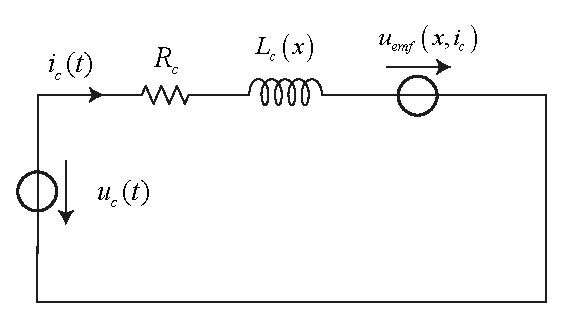
\includegraphics[width = 0.5\textwidth, width = 250pt, angle = 0, keepaspectratio]{figures/equivalent_circuit.eps}
	\captionsetup{width=0.75\textwidth}		
	\caption{Solenoid equivalent electrical circuit.}
	\label{equivalent_circuit_1}
\end{figure}
To complete the solenoid actuator model we must add the mechanical equations using the Newton's equation. To apply the Newton's law we first must calculate the corresponding force actuated by the solenoid.

We first write the \textbf{magnetic coenergy} as
\begin{equation}\label{solenoid_mech_eq_1}
	\begin{split}
		W_m'=\int_{0}^{i_c}\psi(i,x)\,di &= \int_{0}^{i_c}\mu_0H_2\Big(2wd\Big)=\frac{L_0}{1+x/g}i\,di\\[6pt]
		&=\frac{1}{2}\frac{L_0}{1+x/g}i_c^2
	\end{split}
\end{equation}
Hence the force applied to the spool due to the solenoid is as follows
\begin{equation}\label{solenoid_mech_eq_2}
	\begin{split}
		f^v(t)=\frac{\partial W_m'}{\partial x} = -\frac{1}{2}\frac{L_0}{g(1+x/g)^2}i_c^2(t)
	\end{split} 
\end{equation}
The mechanical equations becomes
\begin{equation}\label{solenoid_mech_eq_3}
	\left\lbrace \begin{aligned}
		\frac{dx(t)}{dt} &= v(t) \\[6pt]
		\frac{dv(t)}{dt} &= \frac{1}{2m_v}\frac{L_0}{g\Big(1+x/g\Big)^2}i_c^2(t)-\frac{b}{m_v} v(t)-\frac{k_v}{m_v}\,x(t)
	\end{aligned}\right. 
\end{equation}
Hence the full electromechanical equations of the solenoid actuator become as follows
\begin{equation}\label{solenoid_mech_eq_4}
	\left\lbrace \begin{aligned}
		\frac{dx(t)}{dt} &= v(t) \\[6pt]
		\frac{dv(t)}{dt} &= \frac{1}{2m_v}\frac{L_0}{g\Big(1+\frac{x(t)}{g}\Big)^2}i_c^2(t)-\frac{b}{m_v} v(t) - -\frac{k_v}{m_v}\,x(t)\\[6pt]
		\frac{di_c(t)}{dt} &=-\frac{R_c}{L_0}\Big(1+\frac{x(t)}{g}\Big)i_c(t)+\frac{i_c(t)}{g\Big(1+\frac{x(t)}{g}\Big)}v(t) +\frac{\Big(1+\frac{x(t)}{g}\Big)}{L_0}u_c(t)
	\end{aligned}\right. 
\end{equation}
Now we have to consider two solenoid actuator where:
\begin{equation*}\label{}
	\left\lbrace \begin{aligned}
		x_f &= x_0 - x_v(t) \quad\text{forward solenoid} \quad u_c^f(t)>0,\,u_c^r(t)=0\\[6pt]
		x_r &= x_0 + x_v(t) \quad\text{reverse solenoid} \quad u_c^f(t)=0,\,u_c^r(t)>0
	\end{aligned}\right. 
\end{equation*}
where $x_0=x_v^{\text{max}}$.

The equations which govern the forward solenoid can be represented as follows 
\begin{equation}\label{solenoid_mech_eq_5}
	\left\lbrace \begin{aligned}
		u_c^f(t)&\ge0 \quad \Rightarrow \quad x_v(t)\ge 0 \\[6pt]
		u_c^r(t)&=0\\[6pt]
		\frac{dx_v(t)}{dt} &= v_v(t) \\[6pt]
		\frac{dv_v(t)}{dt} &= \frac{1}{2m_v}\frac{L_0}{g\Big(1+\frac{x_0 - x_v(t)}{g}\Big)^2}\Big[i_c^f(t)\Big]^2-\frac{b}{m_v} v_v(t) - \frac{k_v}{m_v}\,x_v(t)\\[6pt]
		\frac{di_c^f(t)}{dt} &=-\frac{R_c}{L_0}\Big(1+\frac{x_0 - x_v(t)}{g}\Big)i_c^f(t)+\frac{i_c^f(t)}{g\Big(1+\frac{x_0 - x_v(t)}{g}\Big)}v_v(t) +\frac{\Big(1+\frac{x_0 - x_v(t)}{g}\Big)}{L_0}u_c^f(t)
	\end{aligned}\right. 
\end{equation}
while the equations which govern the reverse solenoid can be represented as follows 
\begin{equation}\label{solenoid_mech_eq_6}
	\left\lbrace \begin{aligned}
		u_c^f(t)&=0 \\[6pt]
		u_c^r(t)&>0 \quad \Rightarrow \quad x_v(t)\le 0 \\[6pt]
		\frac{dx_v(t)}{dt} &= v_v(t) \\[6pt]
		\frac{dv_v(t)}{dt} &= -\frac{1}{2m_v}\frac{L_0}{g\Big(1+\frac{x_0 + x_v(t)}{g}\Big)^2}\Big[i_c^r(t)\Big]^2-\frac{b}{m_v} v_v(t) - \frac{k_v}{m_v}\,x_v(t)\\[6pt]
		\frac{di_c^r(t)}{dt} &=-\frac{R_c}{L_0}\Big(1+\frac{x_0 + x_v(t)}{g}\Big)i_c^r(t)+\frac{i_c^r(t)}{g\Big(1+\frac{x_0 + x_v(t)}{g}\Big)}v_v(t) +\frac{\Big(1+\frac{x_0 + x_v(t)}{g}\Big)}{L_0}u_c^r(t)
	\end{aligned}\right. 
\end{equation}






















\clearpage
\begin{thebibliography}{99}
	\bibitem[\textbf{E. Furlani, 2001}]{p1} Edward P. Furlani - \textit{Permanent magnet and electromechanical devices}. Academic Press 2001.	
	\bibitem[\textbf{H. Woodson, 1968}]{p2} H.H. Woodson, J.R. Melcher - \textit{Electromechanical Dynamics, Part I: Discrete Systems}. John Wiley 1968.
	\bibitem[\textbf{H. Woodson, 1968}]{p3} H.H. Woodson, J.R. Melcher - \textit{Electromechanical Dynamics, Part II: Fields, Force and Motion}. John Wiley 1968.
\end{thebibliography}
\end{document} 